\documentclass[
	a4paper
]{scrreprt}

%%% PACKAGES %%%

%etoolbox for rules
\usepackage{etoolbox}

% Figure Placement
\usepackage{float}
% PDF/A Compliance
%\usepackage[a-2b,latxmp]{pdfx}

% add Unicode support and use English as language
\usepackage[utf8]{inputenc}
\usepackage[english]{babel}

% Use Times NR as font
\usepackage{mathptmx}
\usepackage[T1]{fontenc}

% Better tables
\usepackage{tabularx}

% Better enumerisation env
\usepackage{enumitem}
\usepackage{multirow}

% Use graphics
\usepackage{graphicx}

% Have subfigures and captions
\usepackage{subcaption}

% Be able to include PDFs in the file
\usepackage{pdfpages}

% Have custom abstract heading
\usepackage{abstract}

% Need a list of equation
\usepackage{tocloft}
\usepackage{ragged2e}

\usepackage{dirtree}
\usepackage{adjustbox}

% Better equation environment
\usepackage{amsmath}

% Symbols for most SI units
\usepackage{siunitx}

\usepackage{csquotes}

% Clickable Links to Websites and chapters
\usepackage{hyperref}
\hypersetup{hidelinks}

%\addto\extrasngerman{\def\figureautorefname{Abb.}}
%\addto\extrasngerman{\def\tableautorefname{Tabelle}}
\newcommand*{\fullref}[1]{\hyperref[{#1}]{\nameref*{#1} (\ref*{#1})}}


% Change page rotation
\usepackage{pdflscape}

% Symbols like checkmark
\usepackage{amssymb}
\usepackage{pifont}

\usepackage[absolute]{textpos}

% Header
\usepackage{scrlayer-scrpage}

\clearpairofpagestyles
 
 % Configures header and footer
\setkomafont{pageheadfoot}{\rmfamily\footnotesize}
\setkomafont{pagehead}{\rmfamily\bfseries}
\setkomafont{pagination}{}

% Displays line for header and footer
\KOMAoptions{
   headsepline = true,
   footsepline = true,
   plainfootsepline = true,
}

%\usepackage[margin=1cm]{geometry}
\usepackage{pgfgantt}
\usepackage{graphicx}
\usepackage{xcolor}
%\usetikzlibrary{positioning}

\ganttset{group/.append style={orange},
milestone/.append style={red},
progress label node anchor/.append style={text=red}}

\automark[chapter]{chapter}

\ohead{\headmark}
\ihead{Fabian Gröger}

\ofoot*{\pagemark}
\ifoot*{HSLU BAA - Deep embedded Music}

% Glossary, hyperref, babel, polyglossia, inputenc, fontenc must be loaded before this package if they are used
\usepackage[ 
toc,         
acronym,
nopostdot,
sort=standard   
]{glossaries}

\setglossarystyle{listgroup}

% Redefine the quote charachter as we are using ngerman
\GlsSetQuote{+}
% Define the usage of an acronym, Abbreviation (Abbr.), next usage: The Abbr. of ...
\setacronymstyle{long-short}

% Bibliography & citing
\usepackage[
	backend=biber,
	style=apa,
	bibstyle=apa,
	citestyle=apa,
	]{biblatex}
\addbibresource{references_zotero.bib}
\addbibresource{Referenzen.bib}
\addbibresource{Links.bib}
\DeclareLanguageMapping{english}{english-apa}

%%% COMMAND REBINDINGS %%%
\newcommand{\tabitem}{~~\llap{\textbullet}~~}
\newcommand{\xmark}{\ding{55}}
\newcommand{\notmark}{\textbf{\textasciitilde}}
% Pro/Con item https://tex.stackexchange.com/questions/145198/change-the-bullet-of-each-item#145203
\newcommand\pro{\item[$+$]}
\newcommand\con{\item[$-$]}

% Define list of equations - Thanks to Charles Clayton: https://tex.stackexchange.com/a/354096
\newcommand{\listequationsname}{List of Equations}
\newlistof{myequations}{equ}{\listequationsname}
\newcommand{\myequations}[1]{
	\addcontentsline{equ}{myequations}{\protect\numberline{\theequation}#1}
}
\setlength{\cftmyequationsnumwidth}{2.3em}
\setlength{\cftmyequationsindent}{1.5em}

% Usage {equation}{caption}{label}
% \indexequation{b = \frac{\pi}{\SI{180}{\degree}}\cdot\beta\cdot 6378.137}{Bogenlänge $b$ des Winkels $\beta$ mit Radius 6378.137m (Distanz zum Erdmittelpunkt am Äquator)}{Bogenlaenge}
\newcommand{\indexequation}[3]{
	\begin{align} \label{#3} \ensuremath{\boxed{#1}} \end{align}
	\myequations{#3} \centering \small \textit{#2} \normalsize \justify }

% Todolist - credit to https://tex.stackexchange.com/questions/247681/how-to-create-checkbox-todo-list
\newlist{todolist}{itemize}{1}
\setlist[todolist]{label=$\square$}

% Nested Enumeratelist credit to https://tex.stackexchange.com/a/54676
\newlist{legal}{enumerate}{10}
\setlist[legal]{label*=\arabic*.}

%%% GLOSSARY %%%
\loadglsentries{acronyms.tex}
\loadglsentries{glossaries.tex}
\makeglossaries

%%% PATH DEFINITIONS %%%
% Define the path were images are found
\graphicspath{{./img/}{./appendix/}}

% Reset Glossary every chapter
\preto\chapter{\glsresetall}

%%%%%%%%%%%%%%%%
%%% DOCUMENT %%%

\begin{document}

% HSLU Preamble (no header or footer)
\pagestyle{empty}
\begin{titlepage}
	\begin{textblock*}{5cm}[0,0](15.1cm,0.7cm)
		
\includegraphics[keepaspectratio,width=5cm]{img/HSLU_Logo}
	\end{textblock*}
	\begin{center}
		\vspace*{5cm}
		\Huge{\textbf{Deep Embedded Music}} \\
		\vspace{0.5em}
		\Large{Bachelor Thesis FS2020}\\
		\vspace{3em}
		\LARGE{Gröger Fabian}\\
		\vspace{1em}
		\Large{Supervisor: Pfäffli Daniel}\\
		\vfill
		\large{Hochschule Luzern - Departement Informatik}\\
		\large{\today}\\
	\end{center}
	\begin{textblock*}{5cm}[0,0](15.3cm,277mm)
		
\includegraphics[keepaspectratio,width=5cm]{img/FHZ_Logo}
	\end{textblock*}
\end{titlepage}

\newpage

\pagenumbering{gobble}

\begin{textblock*}{5cm}[0,0](15cm,0.7cm)
	
\includegraphics[keepaspectratio,width=2.7cm]{img/HSLU_Logo_Header}
\end{textblock*}

\vspace{0.6cm}
\noindent
\textbf{\Large{Wirtschaftsprojekt an der Hochschule Luzern – Informatik}}

\vspace{0.6cm}
\noindent
\textbf{Titel:} Generierung ansprechender Arbeitszeugnisse

\vspace{0.6cm}
\noindent
\textbf{Studentin / Student:} Barmettler Reto

\vspace{0.6cm}
\noindent
\textbf{Studentin / Student:} Gröger Fabian

\vspace{0.6cm}
\noindent
\textbf{Studiengang:} BSc Informatik

\vspace{0.6cm}
\noindent
\textbf{Jahr:} 2019

\vspace{0.6cm}
\noindent
\textbf{Betreuungsperson:} Pfäffli Daniel

\vspace{0.6cm}
\noindent
\textbf{Expertin / Experte:} Dr. Tim vor der Brück

\vspace{0.6cm}
\noindent
\textbf{Auftraggeberin / Auftraggeber:} confer! AG

\vspace*{1.00cm}

\noindent
\textbf{Codierung / Klassifizierung der Arbeit:} Innovationsprojekte (Projekte mit
Erkenntnisgewinn, Forschungsprojekte)

\begin{todolist}
	\item \textbf{A: Einsicht (Normalfall)}
	\item \textbf{B: Rücksprache}\hspace*{0.7cm}(Dauer:\hspace*{1cm} Jahr / Jahre)
	\item \textbf{C: Sperre}\hspace*{1.865cm}(Dauer:\hspace*{1cm} Jahr / Jahre)
\end{todolist}

\vspace*{1.00cm}

\noindent
\textbf{Eidesstattliche Erklärung}
\\
Ich erkläre hiermit, dass ich/wir die vorliegende Arbeit selbständig und ohne unerlaubte fremde Hilfe angefertigt haben, alle verwendeten Quellen, Literatur und andere Hilfsmittel angegeben haben, wörtlich oder inhaltlich entnommene Stellen als solche kenntlich gemacht haben, das Vertraulichkeitsinteresse des Auftraggebers wahren und die Urheberrechtsbestimmungen der Fachhochschule Zentralschweiz (siehe Markblatt «Studentische Arbeiten» auf MyCampus) respektieren werden.

\vspace{1em}

\noindent
\begin{tabularx}{\textwidth}{@{}lX}
	&\\
	Ort / Datum, Unterschrift: &  \\
	\cline{2-2}
	&\\[0.5cm]
	Ort / Datum, Unterschrift: &  \\
	\cline{2-2}
\end{tabularx}

\begin{textblock*}{5cm}[0,0](14.93cm,277mm)
	
\includegraphics[keepaspectratio,width=5cm]{img/FHZ_Logo}
\end{textblock*}

\newpage

\begin{textblock*}{5cm}[0,0](15cm,0.7cm)
	
\includegraphics[keepaspectratio,width=2.7cm]{img/HSLU_Logo_Header}
\end{textblock*}

\vspace{0.8cm}
\noindent
\textbf{Ausschliesslich bei Abgabe in gedruckter Form: \\ 
Eingangsvisum durch das Sekretariat auszufüllen}

\noindent
\renewcommand{\arraystretch}{2}
\begin{tabularx}{\textwidth}{@{}lXlX}
	Rotkreuz, den & & Visum: & \\
	\cline{2-2}
	\cline{4-4}
\end{tabularx}
\renewcommand{\arraystretch}{1}

\vfill
\noindent
\textbf{Hinweis}: Das Wirtschaftsprojekt wurde von keinem Dozierenden nachbearbeitet.
Veröffentlichungen (auch auszugsweise) sind ohne das Einverständnis der Studiengangleitung der Hochschule Luzern – Informatik nicht erlaubt.

\vspace{1em}

\noindent
\textbf{Copyright} © 2019 Hochschule Luzern - Informatik

\vspace{1em}
\noindent
Alle Rechte vorbehalten. Kein Teil dieser Arbeit darf ohne die schriftliche Genehmigung der Studiengangleitung der Hochschule Luzern - Informatik in irgendeiner Form reproduziert oder in eine von Maschinen verwendete Sprache übertragen werden.


\begin{textblock*}{5cm}[0,0](14.93cm,277mm)
	
\includegraphics[keepaspectratio,width=5cm]{img/FHZ_Logo}
\end{textblock*}


% Rest of the document has header and footer
\pagestyle{headings}
\pagenumbering{Roman}

% Abstract
\begin{abstract}
	\noindent
	Das vorliegende Wirtschaftsprojekt überprüft den Einsatz von Neural Style Transfer für Sätze aus
	der deutschen Sprache. Anhand eines Datensatzes, bestehend aus Sätzen für Erwachsene und Kinder,
	wurde überprüft, ob ein weniger komplexer Satz in einen komplexeren Satz umgewandelt werden kann.
	Die Erkenntnisse sollen dem Auftraggeber als mögliche Grundlage für den Einsatz von Neural Style Transfer 
	für die Verschönerung von Zwischen- und Arbeitszeugnissen dienen.
\end{abstract}

% Table of contents
\tableofcontents

\clearpage
\pagenumbering{arabic}

\chapter{Einleitung}
\label{ch:Einleitung}
In diesem Kapitel wird das Projekt eingeführt, so dass klar wird, was mit der Arbeit erreicht werden soll und aus welchem
Grund diese durchgeführt wird.

\section{Aufgabenstellung und Zielsetzung}
\label{sec:Aufgabenstellung-Zielsetzung}
In dieser Sektion wird die Aufgabenstellung sowie die Zielsetzung des Projektes genauer beschrieben. Ziel ist es,
aufzuzeigen, was genau mit dem Projekt erreicht werden möchte und aus welcher Situation dieses Projekt entstanden ist.
Die ausführliche Aufgabenstellung, welche bei der Transferstelle der Hochschule Luzern eingereicht wurde, ist im Anhang
\fullref{ch:aufgabenstellung} zu finden.

\subsection{Ausgangslage}
\label{sub:ausgangslage}
Mit dem Zeugnismanager der confer! AG können Arbeits- und Zwischenzeugnisse in vier Sprachen erstellt werden. Die
Zeugnisse werden durch einfaches anwählen von Bausteinen zusammengestellt. Die so entstehenden Zeugnisse sind «holprig»
zu lesen. Ein Beispiel ist der Einsatz der Anrede (Frau Meier) und des Personalpronomens (Sie) an geeigneter Stelle.
Solche und ähnliche Problemstellungen werden im Moment mit einfachen Heuristiken gelöst. Weitere Probleme ergeben sich
z. B. durch die unterschiedlichen Grammatiken in den jeweiligen Sprachen. So müssen viele Spezialfälle behandelt werden.

\subsection{Aufgabenstellung}
\label{sub:aufgabenstellung}
Das Ziel ist es, den Zeugnismanager dabei zu unterstützen, sprachlich korrekt ausformulierte Zeugnisse mit einem guten
Lesefluss zu erstellen. Es soll eine Komponente mit Prototypcharakter erarbeitet werden. Der zu erarbeitende Prototyp
kann sich auf eine Sprache, Zeitform und ggf. sogar Geschlecht einschränken, sollte aber entsprechend erweiterbar sein.

\subsection{Zielsetzung}
\label{sub:zeilsetzung}

Wie in der Aufgabenstellung im Anhang \fullref{ch:aufgabenstellung} beschrieben wird, ist das das Projekt ausserhalb des
Tagesgeschäft angesiedelt und Teil von Forschung und Entwicklung. Daher wird das vorliegende Projekt nach einem
explorativen Ansatz durchgeführt. Aus verschiedenen Lösungsansätzen soll ein Ansatz überprüft werden und eine Empfehlung
für den Einsatz beim Arbeitgeber abgegeben werden. Dadurch wird die Zielsetzung und Formulierung der genauen
Problemdefinition im Verlauf der Arbeit vorgenommen. Da es sich um ein exploratives Innovations- / Forschungsprojekt
ist die Erreichung der Aufgabenstellung und Zielsetzung zu Beginn schwer einschätzbar.

\chapter{Stand der Technik}
\label{ch:StandDerTechnik}
In diesem Kapitel werden Begriffe und Konzepte eingeführt und erklärt, welche durch die Arbeit verwendet
werden. Somit kann diese Sektion als ein Nachschalgewerk genutzt werden um allfällige Lücken zu schliessen
und Zusammenhänge zwischen den einzelnen Konzepten besser zu verstehen.

\section{Technologische Grundlagen}
\label{sec:technische-grundlagen}
In diesem Abschnitt werden die wichtigsten technologischen Grundlagen für das Projekt behandelt. Diese Grundlagen
beinhalten vor allem Begriffdefinitionen, welche in den weiteren Kapiteln immer wieder verwendet werden. Die meisten
dieser Grundlagen sind Überbegriffe, welche vorausgesetzt werden um die detaillierten Konzepte in
\fullref{sec:technische-konzepte} zu verstehen.

\subsection{Natural Language Generation}
\label{sub:natural-language-generation}
Natural Language Generation (NLG) (\cite{wikipedia_2019_nlg}) (\textit{dt.} natürliche Textgenerierung), ist ein
Unterbereich von Artificial Intelligence, welcher sich auf die automatisierte Generierung von geschriebenem oder
gesprochenem Text fokussiert.
\newline
\newline
Das Ziel von \gls{NLG} ist es sequenzielle Daten zu generieren, welche nicht von menschlichen Sequenzen unterschieden
werden können. Diese Sätze sollen aussagekräftig und ausserdem grammatikalisch korrekt sein. Dies geschieht in einem
Bruchteil der Zeit welche ein Mensch dafür bräuchte.
\newline
\newline
Etabliert hat sich die Textgenerierung vor allem im Bereich des Journalismus, in denen Nachrichten auf Daten basieren.
So werden heutzutage zum Beispiel Nachrichtentexte für Wetter-, Sport und Finanzberichte zu einem grossen Teil von
NLG-Systemen generiert.

\subsection{Natural Language Processing}
\label{sub:natural-language-processing}
Natural Language Processing (NLP) (\cite{wikipedia_2019_nlp}) (\textit{dt.} natürliche Textverarbeitung) ist ein
Unterbereich von Artificial Intelligence, welcher sich auf die Verarbeitung von natürlicher Sprache fokussiert. Ziel ist
es, eine direkte Kommunikation auf Grund natürlicher Sprache, zwischen dem Menschen und dem Computer herzustellen. NLP
wird z.B. in Sprachassistenten wie Siri oder Alexa verwendet.

\subsection{Neural Style Transfer}
\label{sub:neural-style-transfer}
Der Bereich von \gls{NST} ist eine junge, erst 2015, von Gatys et al. (\cite{gatys2015neural}) eingeführte Technik,
welche sich auf die Manipulation von Bildern bezieht um das Aussehen oder den visuellen Stil eines anderen Bildes zu
übernehmen. \gls{NST} verwenden sehr tiefe Netze, um die Bildtransformation durchzuführen. Häufige Anwendungen für
\gls{NST} sind die Erstellung von künstlichen Kunstwerken aus Fotos, zum Beispiel durch die Übertragung des Aussehens
berühmter Gemälde auf Fotos. \gls{NST} findet die Anwendung vor allem in verschiedenen mobilen Apps.
\begin{figure}[H]
	\centering
	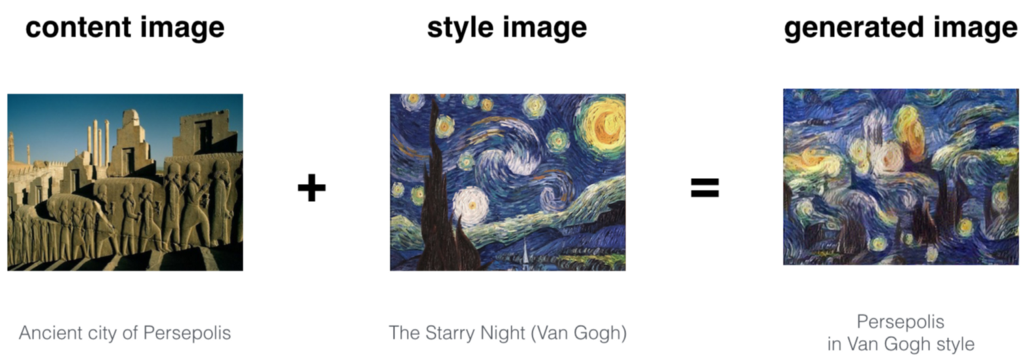
\includegraphics[scale=0.3]{neural_style_transfer}
	\caption{Neural Style Transfer für artistische Gemälde}
	\label{fig:neural-style-transfer}
\end{figure}
\noindent
Infolge des Erfolgs der Technik für artistische Gemälde wurde diese über die Jahre weiter verfolgt. Dabei wird ebenfalls
versucht die Technik auf andere Bereiche anzuwenden. So gibt es eine Bewegung (\cite{fuzhenxin_2019}), die versucht
\gls{NST} auch für Texte zu nutzen. 
\newline
\newline
Dabei werden in der Forschung momentan verschiende \gls{NST} untersucht. Beliebt sind dabei beispielsweise der Transfer
von \flqq positiv\frqq \ zu \flqq negativ\frqq, \flqq informell\frqq \ zu \flqq formell\frqq \ oder auch \flqq
aggressiv\frqq \ zu \flqq passiv\frqq. Dabei wurden in der untersuchten Literatur vorallem die Transfer \flqq
positiv\frqq \ zu \flqq negativ\frqq \ und \flqq informell\frqq \ zu \flqq formell\frqq \ verwendet. In der Tabelle
\ref{tab:beispiele_nst_nlp} sind Beispiele solcher Transfer mit dem \gls{DAST} Modell, \cite{Li2019DomainAT},
aufgelistet.
\begin{table}[H]
	\centering
	\begin{tabular}{|c|c|}
		\hline
		\multicolumn{2}{|c|}{\textbf{Positiv} $\rightarrow$ \textbf{Negativ} } \\
		\hline
		\textbf{Eingabe} &  the service was great , food delicious , and the value impeccable . \\
		\textbf{Ausgabe} & the service was horrible , food bland , and the value lousy . \\
		\hline
		\multicolumn{2}{|c|}{\textbf{Negativ} $\rightarrow$ \textbf{Positiv}} \\
		\hline
		\textbf{Eingabe} & the service was horrible , food bland , and the value lousy . \\
		\textbf{Ausgabe} & and the pizza was tasty , juicy , and definitely quite amazing . \\
		\hline
	\end{tabular}
	\caption{Beispiele eines \gls{NST} mit Stil \flqq positiv \frqq \ und \flqq negativ \frqq \ mit dem \gls{DAST} Modell}
  \label{tab:beispiele_nst_nlp}
  \end{table}
\noindent
\newline
Bei einem \gls{NST} wird versucht für einen Input $ x = x_{content} + x_{style} $ eine Repräsentation $
\widetilde{x} = \widetilde{x}_{content} + \widetilde{x}_{style} $ für den Zielstil $ Y_{style} $ zu finden. Die
Transformation soll dabei Werte für $ \widetilde{x}_{content} $ und $ \widetilde{x}_{style} $ finden so, dass
\begin{equation}
	\widetilde{x}_{content} = x_{content} \qquad und \qquad \widetilde{x}_{style} = Y_{style}
\end{equation}
\myequations{Style Transfer Variablen Definition}
\noindent
Damit ist das Finden von $ \widetilde{x} $ ein Minimierungsproblem der Distanzen.
\begin{equation}
	\arg\min \widetilde{x} = |\widetilde{x}_{content} - x_{content}| + |\widetilde{x}_{style} - Y_{style}|
\end{equation}
\myequations{Style Transfer Loss Funktion}
\noindent
\newline
Um nun diese Technik anzuwenden, muss entsprechend einen Messung für Inhalt ($ content $) und Stil ($ style $) definiert
werden.

\subsection{Künstliche neuronale Netze}
\label{sub:neural-nets}
Künstliche neuronale Netze sind spezielle Typen von Machine Learning Modellen, die von der Funktionsweise des
menschlichen Gehirns inspiriert sind. Künstliche neuronale Netze sind von biologischen neuronalen Netzen
inspiriert, unterscheiden sich jedoch in vielerlei Hinsicht. Der Vergleich wird im Bild \fullref{fig:ANN-NN} anschaulich
dargestellt. Ein \gls{KNN} besteht aus Berechnungseinheiten, den Neuronen, sowie Verbindungselementen,
den Synapsen, welche Neuronen miteinander verbinden und ein Gewicht enthalten. 
\newline
Wenn ein Neuron eine Zahl als Eingabe erhält, wird eine Art von Berechnung durchgeführt (z.B. eine Sigmoid
Aktivierungsfunktion) und anschliessend wird das Ergebnis mit dem Gewicht der Synapse zum nächsten Neuron multipliziert,
wenn es sich \flqq aktiviert\frqq.
\begin{figure}[H]
	\centering
	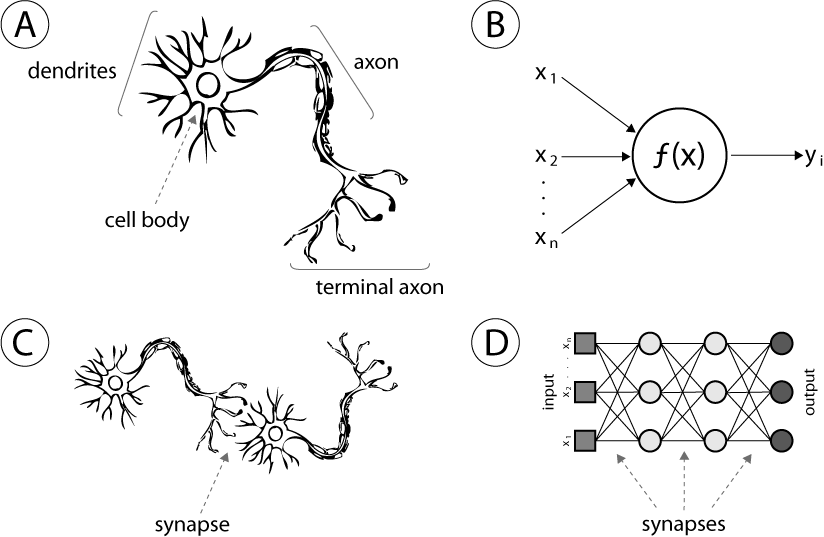
\includegraphics[scale=0.4]{ANN-NN}
	\caption{Unterschied zwischen einem ANN und einem NN \href{http://www.intechopen.com/source/html/39067/media/image1.png}{(source)}}
	\label{fig:ANN-NN}
\end{figure}
\noindent
Sie bieten eine alternative Möglichkeit zu den linearen Modellen der Datenverarbeitung. Die Neuronalen Netze modellieren
eine nicht lineare Beziehung zwischen Ein- und Ausgängen. Somit kann sich das Modell den Daten entsprechend anpassen,
egal wie die Daten verteilt sind. Es kann jede versteckte, mathematische Funktion zwischen den Daten und dem Ergebnis
erkennen und erlernen. Ein Problem der neuronalen Netze ist die enorme Menge an Rechenressourcen und Daten, die benötigt
werden, um gut zu funktionieren.
\newline
\newline
\textbf{Deep Neural Networks} ist eine weitere From von neuronalen Netzen. Der einzige Unterschied besteht darin, dass
\textit{deep neural network} mehrere hidden Layers haben und somit komplexere mathematische Zusammenhänge lernen
können. Diese Netzwerke kommen vor allem in der Bilderkennung zum Einsatz. Ein gutes Beispiel des Einsatzes eines
\textit{deep neural network} ist, die Erkennung von verschiedenen Gesichtern mittels einer Verkehrskamera. 
\newline
\newline
Einer der grössten Nachteile eines Neuronalen Netzes ist, dass es nicht weiss, welche Ereignisse vorher passiert sind.
Das heisst, es hat keine Erinnerungen an vergangene Handlungen. Im Bereich \gls{NLP} und \gls{NLG} ist dieser Nachteil
sehr bedeutsam, denn ohne sich an das vorher Geschehene zu erinnern, kann man keine Vorhersagen über zukünftige
Ereignisse treffen. Aus diesem Grund wurden spezielle neuronale Netze entwickelt, die eine Art von Gedächtnis haben, wie
zum Beispiel \gls{RNN} \ref{sub:rnn} oder LSTMs \ref{sub:lstm}, welche im nächsten Abschnitt genauer beschrieben werden.

\subsubsection{Prezeptron}
\label{sub:preceptron}
Künstliche neuronale Netze sind kein neues Konzept, anfänglich hiessen diese \flqq Prezeptronen\frqq \ und wurden
bereits um 1960 entwickelt. Diese Prezeptronen bestanden aus sogenannten McCulloch-Pitts-Neuronen. Diese wurden stetig
weiterentwickelt und es entstanden gewichtete, sowie mehrschichtige Prezeptronen, aus denen die heutigen künstlichen
neuronalen Netze entstanden.

\subsubsection{Aufbau}
\label{sub:structure-nn}
Neuronale Netze haben immer eine ähnliche Grundstruktur, sie bestehen aus sogenannten Schichten (\textit{eng.} Layers).
Diese Schichten sind einfache Gruppen von Neuronen, welche mittels Synapsen mit einer anderen Gruppe von Neuronen
verbunden sind. Die grundsätzliche Struktur eines \gls{ANN} beinhaltet eine Eingabeschicht (\textit{eng.} input layer),
mehrere versteckte Schichten (\textit{eng.} hidden layers) und eine Ausgabeschicht (\textit{eng.} output layer). In der
Eingabeschicht werden die Daten dem neuronalen Netz zur Verarbeitung gegeben. Die versteckten Schichten bestehen aus
mehreren Schichten von Neuronengruppen, welche die zu grundeliegende mathematische Funktion der Daten lernen. Am Schluss
hat jedes Netz noch eine Ausgabeschicht, wo die Resultate des Netzes ausgegeben werden. Dieser output layer hat immer
die Grösse des gewünschten Ergebnisses, d.h. wenn man ein \gls{NN} trainieren möchte um zwischen gesunden und
kranken Zellen zu unterscheiden, wird die Ausgabeschicht zwei Neuronen beinhalten.
\begin{figure}[H]
	\centering
	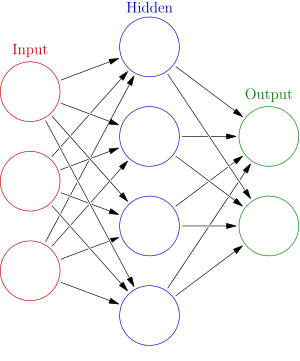
\includegraphics[scale=0.4]{NN_Structure}
	\caption{Struktur eines neuronalen Netzes \href{https://upload.wikimedia.org/wikipedia/commons/thumb/4/46/Colored_neural_network.svg/300px-Colored_neural_network.svg.png}{(source)}}
	\label{fig:NN-Structure}
\end{figure}

\subsubsection{Training}
\label{sub:training-nn}
Ein \gls{KNN} muss trainiert werden um die richtigen Berechnungen und die richtigen Gewichte in den
einzelnen Neuronen und Synapsen zu setzen. Dieses Training funktioniert im \textit{Supervised Learning} so, dass dem
\gls{KNN} eine vielzahl an Beispielen gegeben wird. Das neuronale Netz versucht dann, die gleichen Antworten wie im
Beispiel zu erhalten. Wenn es eine falsche Antwort voraussagt, wird ein Fehler berechnet und die Werte an jedem Neuron
und jeder Synapse werden für das nächste Mal rückwärts durch das \gls{NN} propagiert. Diesen Prozess nennt man
\textbf{Backpropogation} und wird in jedem \gls{KNN} verwendet, um die einzelnen Parameter anzupassen.

\subsubsection{Loss Funktion}
\label{sub:loss_fkt}
Das in \ref{sub:training-nn} beschriebene Training behilft sich einer sogenannten Loss Funktion um die Gewichte des
Netzes anzupassen. Dies ist eine Funktion um zu evaluieren, wie gut die aktuelle nichtlineare Funktion des \gls{KNN} die
Daten repräsentiert. Wenn die Vorhersagen des \gls{NN} weit von den echten Daten entfernt sind, gibt die Loss Funktion
einen hohen Wert aus. Wenn diese allerdings einigermassen ähnlich sind, ist der Wert der Funktion gering. 
\newline
\newline
Es wird zwischen Regression Loss und Classification Loss unterschieden. Regression Loss Funktionen
werden gebraucht bei Vorhersagen für kontinuierliche Werte. Classification Loss Funktionen werden gebraucht bei
Vorhersagen von kategorischen Labels, zum Beispiel ob es sich auf einem Bild um eine Katze oder einen Hund handelt.
\newline
\newline
Diese Funktion wird minimiert um ein möglichst gutes Ergebnis zu erhalten, dies geschieht mittels einem Optimizer
welcher in der Sektion \ref{sub:optimizer} genauer beschrieben wird.

\subsubsection{Optimizer}
\label{sub:optimizer}
Ein Optimizer im \gls{KNN} macht im Grunde nichts anderes als die \fullref{sub:loss_fkt} zu Optimieren indem diese
minimiert wird. Durch das kontinuierliche Minimieren der Loss Funktion performt das Modell nach jeder Iteration besser
und sucht die optimale Funktion um die Daten zu repräsentieren. Die Gewichte des \gls{NN} müssen nach jeder Iteration so
angepasst werden, dass die Loss Funktion, welche mittels dem Output berechnet wird, minimiert wird. Diese Anpassung kann
zum Beispiel mittels der Partiellen Ableitung der einzelnen Gewichte mit Respekt zum Loss berechnet werden. Dieser
spezielle Optimizer wird auch Gradient Descent genannt.

\section{Technische Konzepte}
\label{sec:technische-konzepte}
In diesem Abschnitt werden technische Konzepte genauer erklärt, welche in der Arbeit verwendet wurden. Diese Konzepte
sind meist sehr umfangreich und werden daher nur angeschnitten, so dass die weiteren Schlüsse dieser Arbeit
nachvollziehbar verstanden werden können.

\subsection{Markov Chains}
\label{sub:markov_chains}
Markov-Ketten gehören zu den frühesten Algorithmen im Bereich der Natural Language Generation. Sie sagen das nächste
Wort in einem Satz voraus, indem sie einfach das aktuelle Wort verwenden. Eine Markov-Kette berücksichtigt die Beziehung
zwischen jedem einzelnen Wort, um die Wahrscheinlichkeit des nächsten Wortes zu berechnen. Sie wurden in früheren
Versionen von Smartphone-Tastaturen verwendet, um Vorschläge für das nächste Wort im Satz zu generieren.
\newline
\newline
In Abbildung \ref{fig:markov-example} wird eine solche Kette anhand eines Beispiels von
\cite{andrew_adventure_markov_chain} dargestellt. Die Datensätze für die Markov Kette sind: \flqq I like turtles\frqq,
\flqq I like rabbits\frqq und \flqq I don't like snails\frqq. Die Abbildung \ref{fig:markov-example} bedeutet:
\begin{enumerate}
	\setlength\itemsep{0em}
	\item die Sätze zu 100\% mit einem \textit{I} starten
	\item gefolgt von einem \textit{like} zu 66\% und 33\% einem \textit{don't}
	\item das Wort \textit{don't} wird zu 100\% gefolgt von einem \textit{like}
	\item zum Schluss des Satzes gibt es zu 33\% entweder ein \textit{rabbits}, \textit{turtles} oder \textit{snails}
\end{enumerate}
\begin{figure}[H]
	\centering
	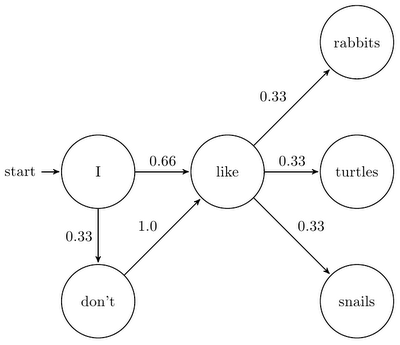
\includegraphics[scale=0.5]{markov_example}
	\caption{Visualisierung einer Markov Chain für Sequenzen}
	\label{fig:markov-example}
\end{figure}

\subsection{Recurrent Neural Networks}
\label{sub:rnn}
\gls{RNN} gehören zu den neusten Errungenschaften im Bereich der Neuronalen Netzen. Sie erlauben es, lange Sätze
zu verarbeiten mit einer deutlichen Verbesserung der Genauigkeit. \gls{RNN} ist eine spezielle Art der neuronalen
Netzwerke, welche sich die sequenzielle Natur der Eingabe zu nutzen macht. Jeder einzelne Teil der Sequenz (z.B. ein
Satz oder ein Vers) durchläuft ein Feedforward-Netzwerk und gibt die Ausgabe des Modells als Input für den nächsten Teil
der Sequenz, wie in Grafik \ref{fig:RNN-Overview} gut ersichtlich ist. Dies ermöglicht die Speicherung von Informationen aus
vorherigen Schritten, wie eine Art von Gedächtnis.
\newline
\newline
Durch dieses Gedächtnis über vorherige Schritte sind \gls{RNN} besonders beliebt bei Sprachgenerierung, da sie sich an den
Kontext des Satzes oder des Gespräches im Laufe der Zeit erinnern können. Aber nicht nur bei der Sprachgenerierung sind
\gls{RNN} beliebt, sondern auch bei: Spracherkennungen, Sprachmodellierungen und Übersetzungen.
\newline
\newline
\gls{RNN} haben einen grossen Nachteil, nämlich das Problem des verschwindenden Gradienten (\textit{eng.} \ \flqq
vanishing gradient problem\frqq). Mit zunehmender Länge der Sequenz verliert das Netzwerk die Erinnerung an Wörter die
weit zurück liegen und somit werden die Vorhersagen nur auf Grund von neuen Wörtern getroffen. Um dieses Problem zu
lösen wurden \gls{LSTM} \ref{sub:lstm} entwickelt, welche dieses Problem geschickt lösen.
\begin{figure}[H]
	\centering
	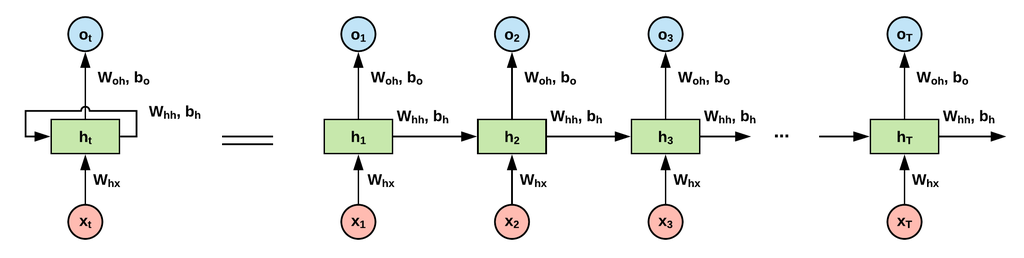
\includegraphics[scale=1.5]{RNN_Overview}
	\caption{Visualisierung eines RNN}
	\label{fig:RNN-Overview}
\end{figure}

\subsection{Long Short-Term Memory}
\label{sub:lstm}
\gls{LSTM} sind eine spezielle Art von Recurrent Neural Networks und somit auch eine Art von neuronalen Netzen. Die \gls{LSTM}
sind darauf ausgelegt, dass sie mit langen Sequenzen von Wörtern genauer arbeiten können. \gls{LSTM} unterscheiden sich von
herkömmlichen \gls{RNN} in einem wichtigen Punkt, nämlich haben die \gls{LSTM} ein vierschichtiges \gls{NN}. Normale
\gls{RNN} haben nur ein einschichtiges Netzwerk. Die kettenartige Struktur wurde auch in den \gls{LSTM}
gebraucht.
\newline
\newline
Das \gls{LSTM} hat die Fähigkeit, Informationen vom Zellzustand zu entfernen oder hinzuzufügen, welche sorgfältig durch
Strukturen reguliert werden, die als Gates bezeichnet werden. Gates sind eine Möglichkeit, Informationen optional
durchzulassen. Sie bestehen aus einer sigmoiden neuronalen Netzschicht und einer punktweisen Multiplikationsoperation,
wie in der Abbildung \ref{fig:LSTM-Gate} zu sehen ist. Die sigmoide Schicht des Netzwerks gibt eine Zahl zwischen Null
und Eins aus, welche beschreibt wie viel von dem Vektor durchgelassen werden soll. Ein Wert von Null bedeutet, dass
nichts durchgelassen werden soll und ein Wert von Eins bedeutet, dass alles durchgelassen werden soll. Ein \gls{LSTM}
hat drei solcher Gates um den Zellzustand zu kontrollieren.
\newline
\begin{figure}[H]
	\centering
	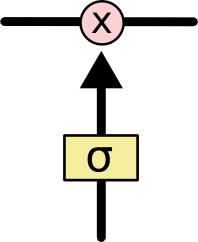
\includegraphics[scale=1]{LSTM_Gate}
	\caption{Visualisierung eines LSTM Gates \href{http://colah.github.io/posts/2015-08-Understanding-LSTMs}{(Colah's Blog)}}
	\label{fig:LSTM-Gate}
\end{figure}
\noindent
Ein Long Short-Term Memory besteht aus vier Komponenten, wie man der Grafik \ref{fig:LSTM-Overview} entnehmen kann:
\begin{enumerate}
	\setlength\itemsep{0em}
	\item einer Zelle (cell), beinhaltet den Zellzustand
	\item einem Eingangsgate (input gate)
	\item einem Ausgangsgate (output gate)
	\item einem Vergessensgate (forget gate)
\end{enumerate}
Diese Komponenten ermöglichen es dem Netzwerk, Wörter über beliebige Zeitintervalle zu merken oder diese auch wieder zu
vergessen, indem sie selber den Informationsfluss in und aus der Zelle regeln können. In der Zelle werden die
Informationen über vorgängige wichtige Wörter gespeichert, so dass auf diese zu einem späteren Zeitpunkt zugegriffen
werden können. Ausserdem kann das Netzwerk erkennen, wann ein Satzende eingetroffen ist und sich der Kontext ändert.
Durch diese Feststellung können durch das Vergessensgate Informationen übersprungen werden, welche in diesem Kontext für
nicht mehr relevant angeschaut werden. Dies ermöglicht es dem Netzwerk, selektiv nur relevante Informationen zu
verfolgen und gleichzeitig Informationen über einen längeren Zeitraum zu speichern.
\newline
\begin{figure}[H]
	\centering
	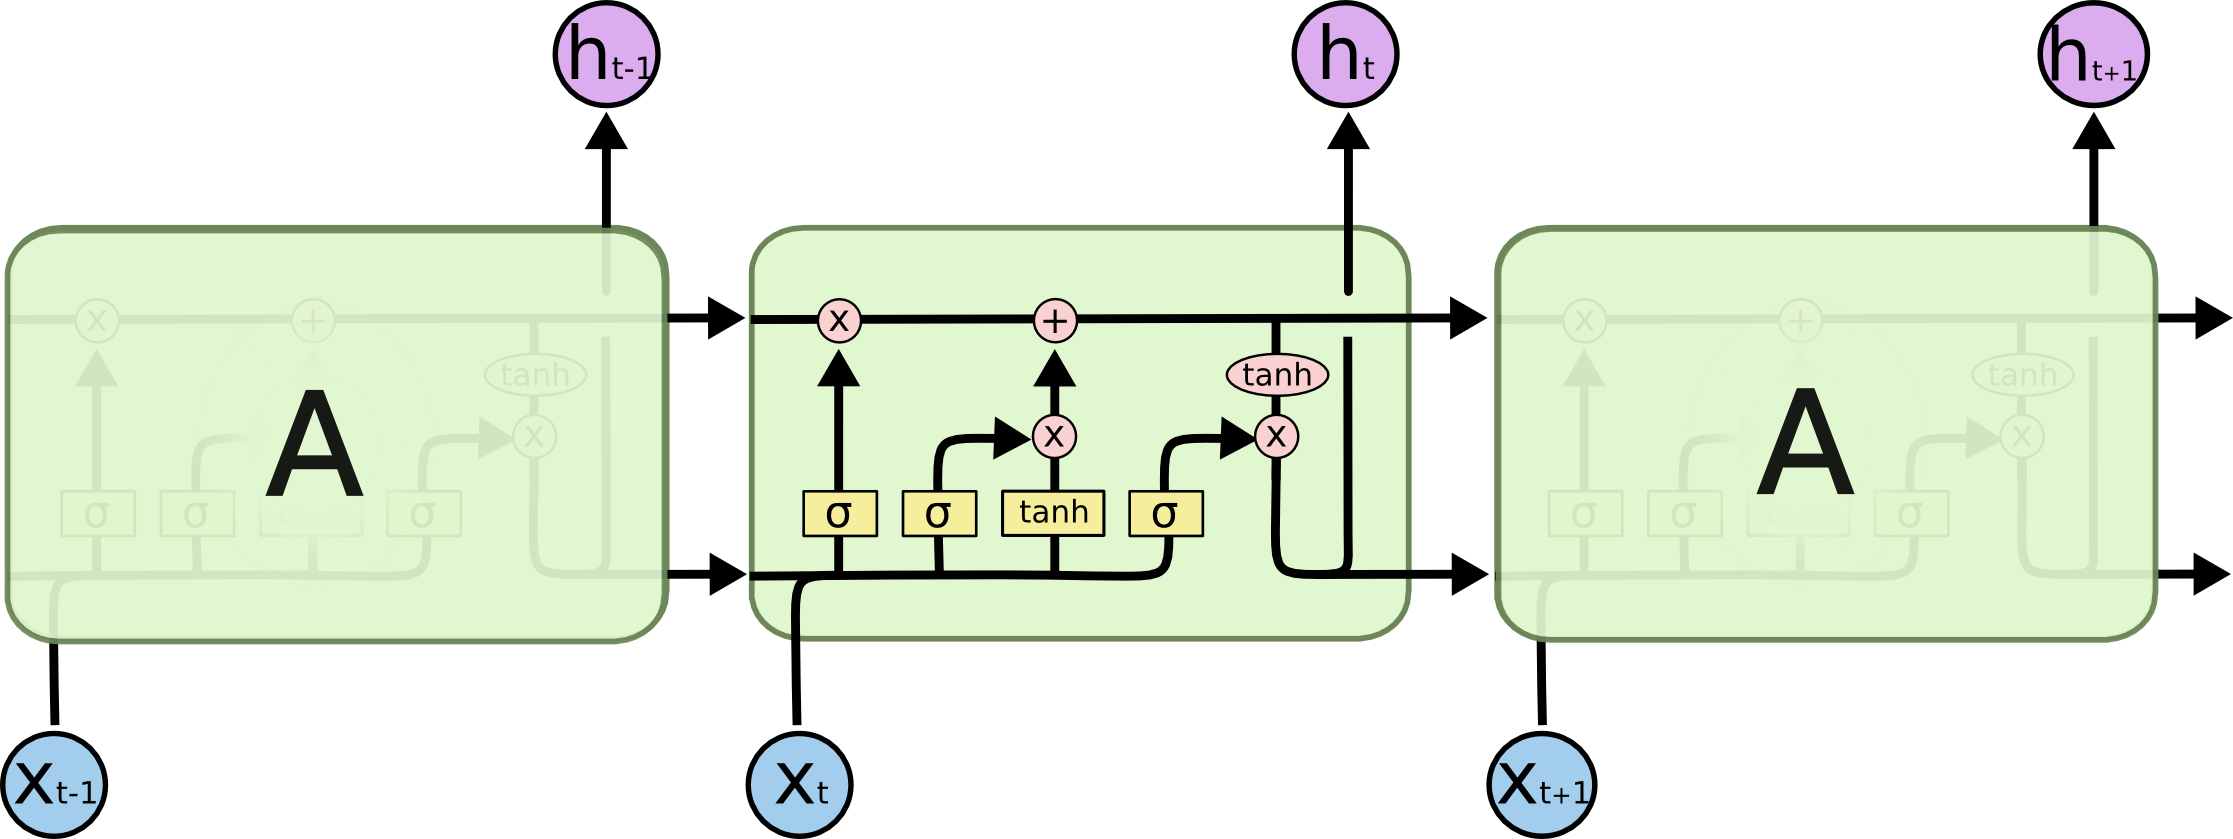
\includegraphics[scale=0.4]{LSTM_Overview_New}
	\caption{Visualisierung eines LSTM \href{http://colah.github.io/posts/2015-08-Understanding-LSTMs}{(Colah's Blog)}}
	\label{fig:LSTM-Overview}
\end{figure}
\noindent
\gls{LSTM} und ihre Variationen schienen die Antwort auf das \flqq vanishing gradient problem\frqq \ zu sein, jedoch gibt es
auch bei diesen Netzwerken gewisse Einschränkungen wie viele Informationen effektiv gespeichert werden können. Denn es
muss immer noch ein komplexer sequentieller Pfad der letzten Zelle zur nächsten Zelle übergeben werden. Dadurch
beschränkt sich die Länge der Sequenz, an die sich ein \gls{LSTM} noch erinnern kann, auf wenige hundert Wörter.
\newline
\newline
Ein weiterer Nachteil ist, dass \gls{LSTM} aufgrund ihrer hohen Rechenanforderungen sehr schwer zu trainieren sind. Aufgrund
ihrer sequentiellen Natur sind sie schwer zu parallelisieren und können somit den Vorteil der heutigen Rechengeräten wie
\gls{GPU} und \gls{TPU} nicht ausgiebig nutzen.

\subsubsection{Ablauf eines Schrittes im LSTM}
\label{sub:lstm-step-by-step}
\begin{figure}[H]
	\centering
	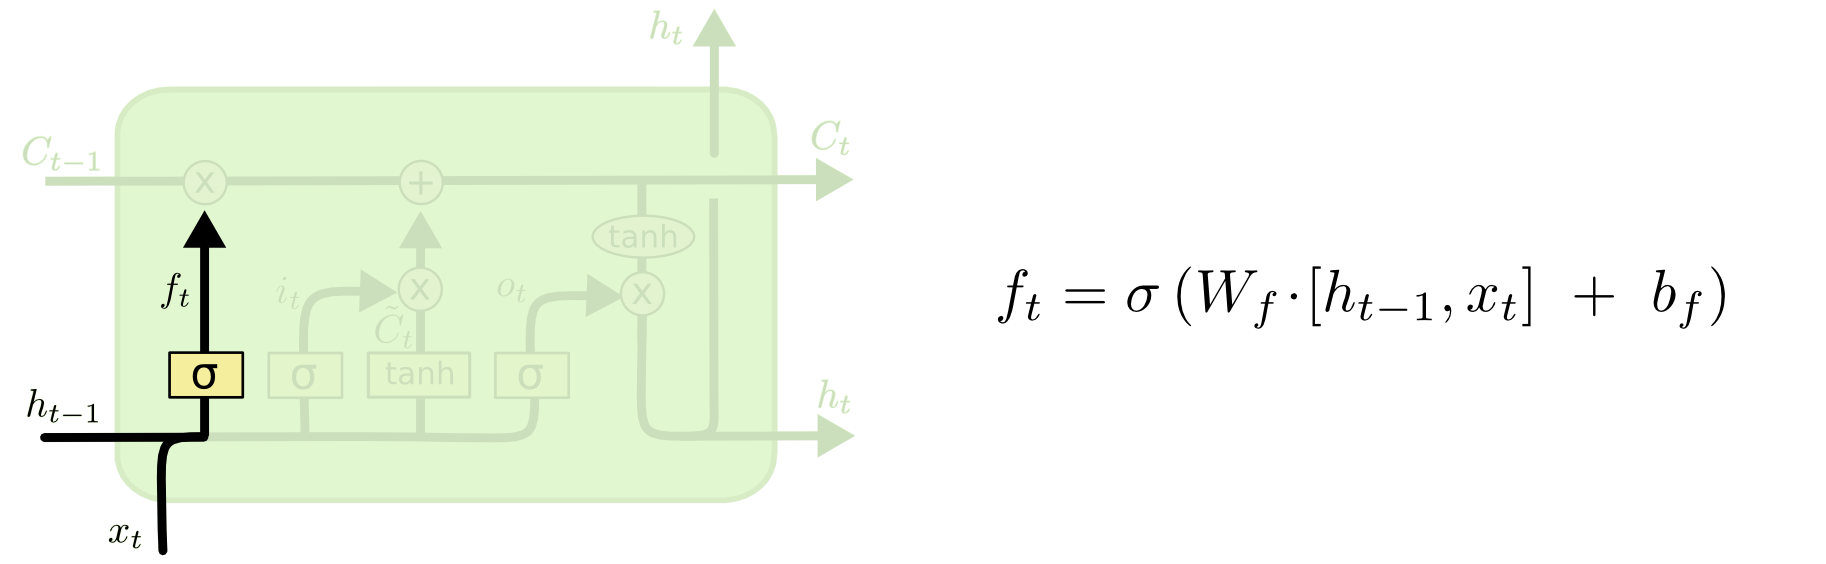
\includegraphics[scale=0.4]{LSTM_Forgetgate}
	\caption{Visualisierung eines LSTM Vergessensgates \href{http://colah.github.io/posts/2015-08-Understanding-LSTMs}{(Colah's Blog)}}
	\label{fig:LSTM-Forgetgate}
\end{figure}
\noindent
Der erste Schritt in einem \gls{LSTM} ist es zu entscheiden, welche Informationen aus der Zelle verworfen werden. Diese
Entscheidung wird durch die Sigmoid Funktion des Vergessensgates getroffen. Es schaut sich den Input $x_t$ und den
Output des vorherigen Wortes $h_{t-1}$ an und gibt eine Zahl zwischen $0$ bis $1$ aus für jeden einzelne Komponente des
Zellzustandvektor $C_{t-1}$. Eine $1$ bedeutet, dass der Wert komplett behalten werden soll. Eine $0$ hingegen bedeutet,
dass der Wert komplett verworfen werden soll. Dadurch entsteht ein \flqq Vergessensvektor\frqq \ $f_t$.
\newline
\begin{figure}[H]
	\centering
	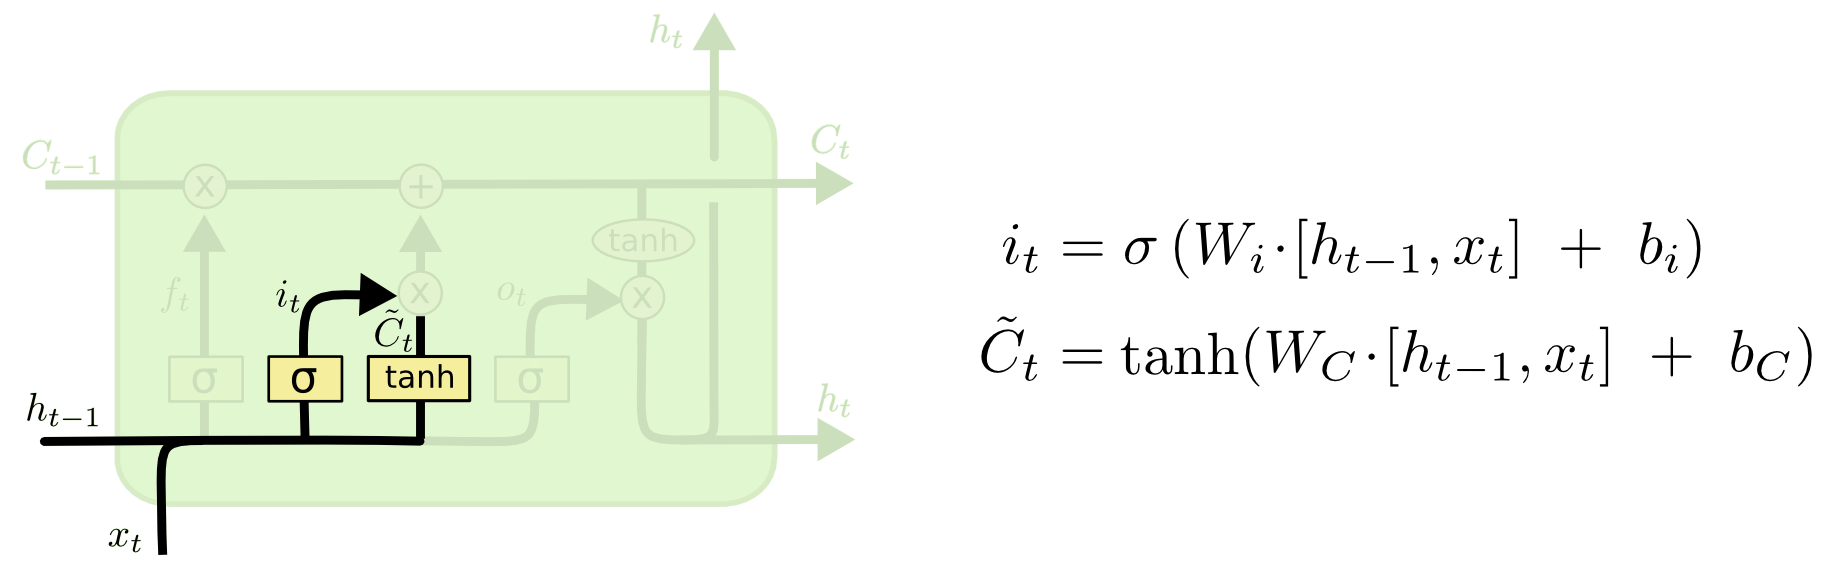
\includegraphics[scale=0.4]{LSTM_Inputgate}
	\caption{Visualisierung eines LSTM Eingangsgates \href{http://colah.github.io/posts/2015-08-Understanding-LSTMs}{(Colah's Blog)}}
	\label{fig:LSTM-Inputgate}
\end{figure}
\noindent
In einem nächsten Schritt wird darüber entschieden, welche neuen Informationen im Zellzustand gespeichert werden. Diese
Entscheidung wird in zwei Schritten getroffen. Als Erstes entscheidet die Sigmoid Funktion des Eingangsgates, welche
Werte aktualisiert werden und erstellt einen \flqq Aktualisierungsvektor\frqq \ $i_t$, welcher für jeden Wert des
Zellzustands eine Zahl zwischen $0$ und $1$ beinhaltet. Als nächstes erstellt eine Tanh Funktion einen neuen
Zellzustandvektor $\tilde{C}_t$ mit den aktualisierten Werten des Zustands. In einem nächsten Schritt werden die beiden
Vektoren $i_t$ und $\tilde{C}_t$ kombiniert und der Zellzustand wird aktualisiert.
\newline
\newline
Anschliessend wird der alte Zellzustand $C_{t-1}$ zum neuen Zustand $C_t$ aktualisiert. Der alte Zustand wird mit dem
berechneten \flqq Vergessensvektor\frqq \ $f_t$ multipliziert, um die Dinge zu vergessen, die irrelevant geworden sind.
Dann multiplizieren wir das Ergebnis des vorherigen Schrittes mit dem \flqq Aktualisierungsvektor\frqq \ $i_t$
kombiniert mit dem neuen Zellzustandvektor $\tilde{C}_t$. Aus dem ergibt sich der neue Zellzustand $C_t$.
\newline
\begin{figure}[H]
	\centering
	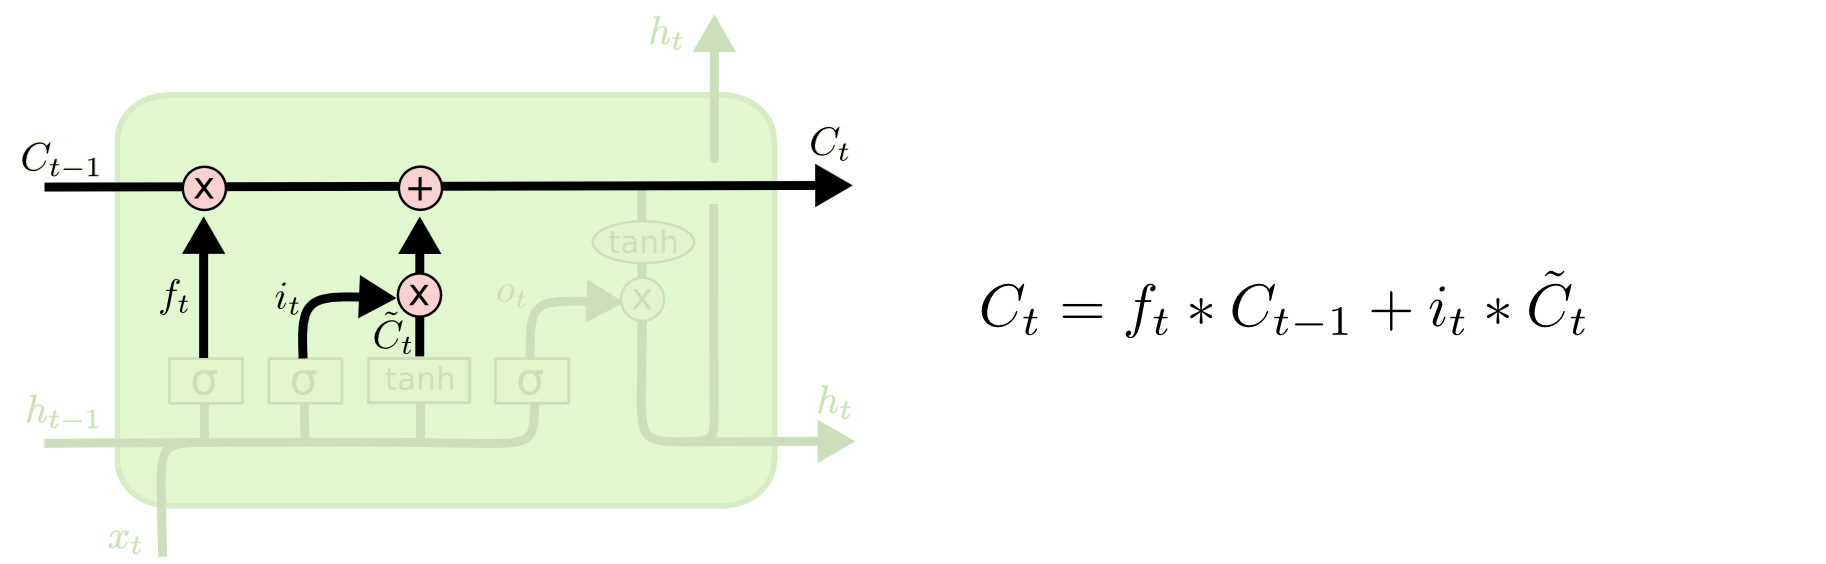
\includegraphics[scale=0.4]{LSTM_Addition}
	\caption{Visualisierung der Addition der Vektoren eines LSTMs \href{http://colah.github.io/posts/2015-08-Understanding-LSTMs}{(Colah's Blog)}}
	\label{fig:LSTM-Addition}
\end{figure}
\noindent
Schliesslich muss entschieden werden, was ausgegeben werden soll, diese Entscheidung wird im Ausgangsgate getroffen. Der
Output basiert auf dem neuen Zellzustandvektor $C_t$, wird aber vorgängig noch gefiltert. Zuerst wird eine Sigmoid
Funktion auf dem Input $x_t$ und dem Output des vorherigen Wortes $h_{t-1}$ ausgeführt, um zu entscheiden welche Teile
des Zustandes ausgegeben werden. Dann wird der aktuelle Zellzustand $C_t$ mittels einer Tanh Funktion auf die Werte
zwischen $-1$ und $1$ gebracht und anschliessend mit dem Resultat der Sigmoid Funktion multipliziert. Somit werden nur
die Teile ausgegeben, die wirklich relevant sind.
\newline
\begin{figure}[H]
	\centering
	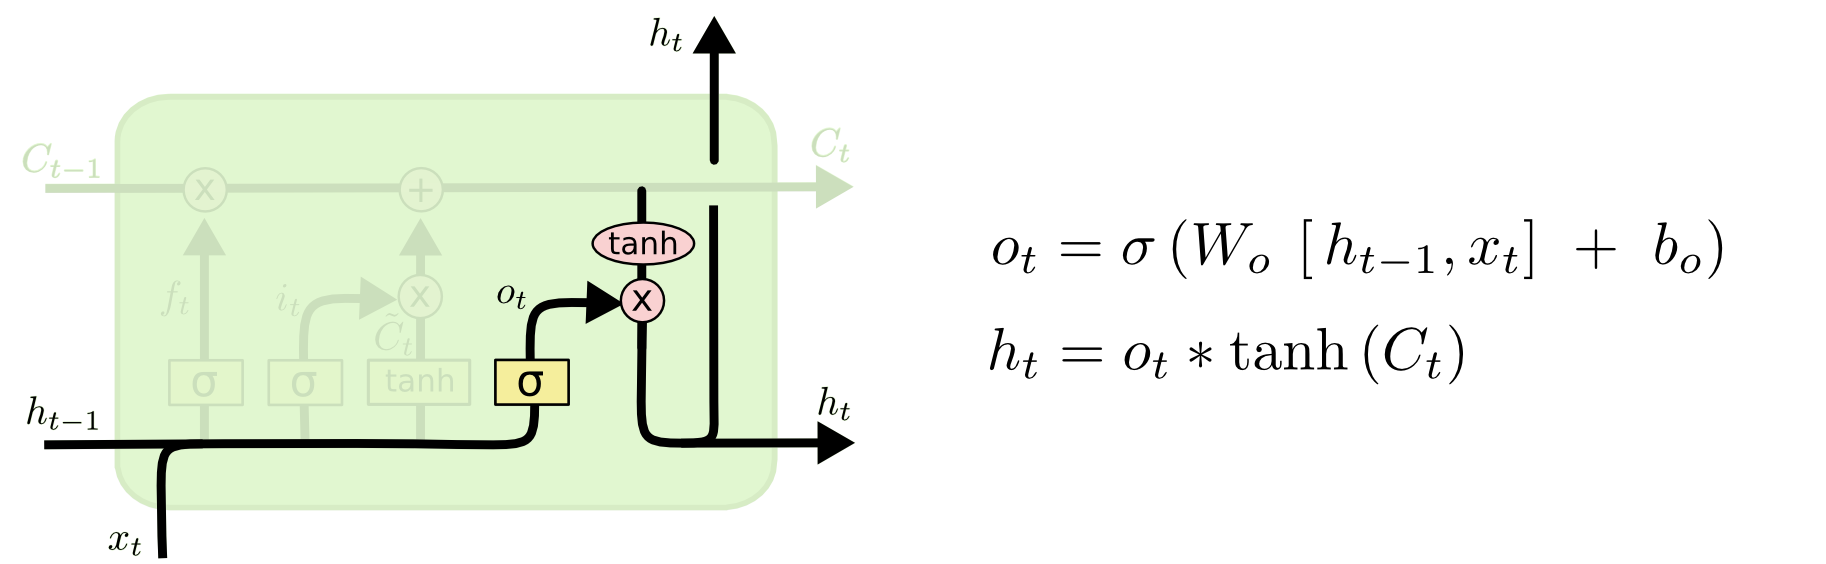
\includegraphics[scale=0.4]{LSTM_Outputgate}
	\caption{Visualisierung eines LSTM Ausgangsgate \href{http://colah.github.io/posts/2015-08-Understanding-LSTMs}{(Colah's Blog)}}
	\label{fig:LSTM-Outputgate}
\end{figure}

\subsection{Autoencoder}
\label{sub:autoencoder}
Autoencoder sind eine spezielle Art von \gls{KNN}, welche oft verwendet werden, um effiziente
Datencodierungen auf unbeaufsichtigte (unsupervised) Weise zu erlernen. Ein Autoencoder besteht auf der einen Seite aus
einem Encoder und auf der anderen aus einem Decoder. 
\newline
\newline
Das Ziel des Encoders ist es, eine Darstellung für einen Datensatz zu erlernen, typischerweise mit dem Zweck der
Reduzierung der Dimensionalität. Indem das Netzwerk trainiert wird, lernt es das Rauschen oder Unreinheiten zu
ignorieren und sich auf die echten Daten zu konzentrieren.
\newline
\newline
Der Decoder hat das Ziel, aus der reduzierten Codierung eine Darstellung zu rekonstruieren, die seiner ursprünglichen
Form so nahe wie möglich kommt.
\newline
\newline
Durch diese Eigenschaft der Komprimierung und der Rekonstruktion werden Autoencoder effektiv zur Lösung vieler Probleme
eingesetzt, von der Gesichtserkennung bis zum Erlangen der semantischen Bedeutung für die Worte.
\begin{figure}[H]
	\centering
	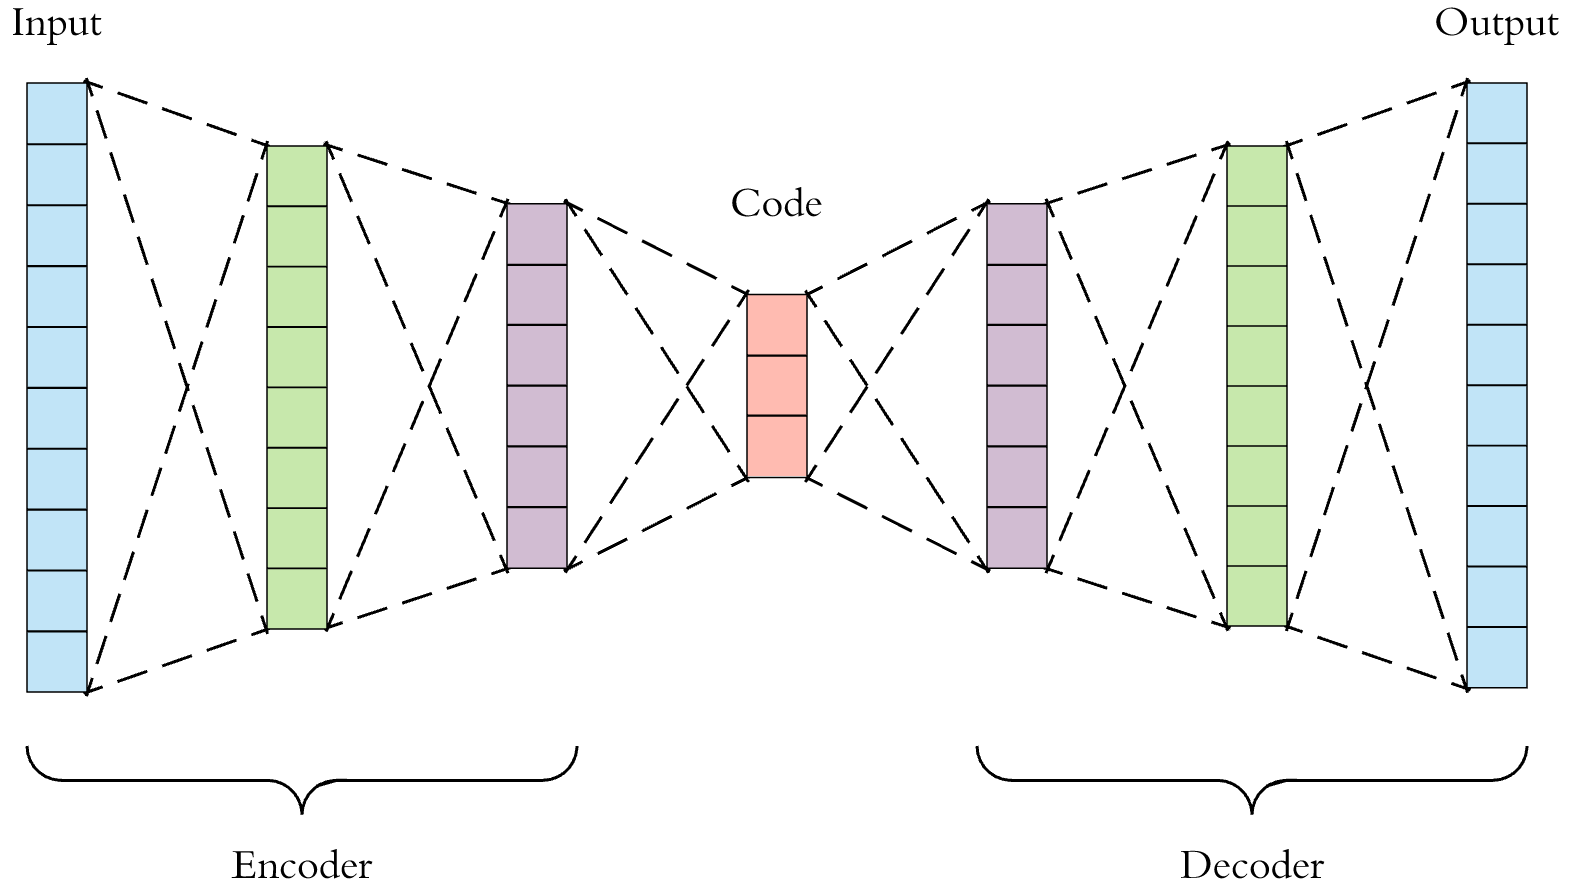
\includegraphics[scale=0.2]{autoencoder}
	\caption{Visualisierung eines Autoencoders}
	\label{fig:Autoencoder}
\end{figure}

\subsection{Transformer}
\label{sub:transformer}
Transformer sind eine weitere Art von \gls{KNN}, welche sehr intuitiv verstanden werden können. Die
Hauptaufgabe besteht darin, einen Input (z.B. einen deutschen Satz) in einen Output (z.B. in einen englischen Satz) zu
transformieren. Das Transformermodell besteht aus mehreren Encoder- und Decoder Komponenten, welche zusammen verbunden
sind. Die Encoder Komponenten sind nichts weiteres als mehrere Encoders, welche aufeinander gestapelt werden und eine
Verbindung zum oberen Encoder haben. Dasselbe wird auch bei der Decoder Komponente gemacht, dort werden mehrere
Decoders aufeinander gestapelt und sind mit dem oberen Layer verbunden. Der oberste Encoder der Encoder Komponente ist
mit jedem Decoder der Decoder Komponente verbunden. Dem ersten Encoder wird der Input übergeben und der letzte Decoder
liefert den gewünschten Output.
\newline
\newline
Transformatoren wurden entwickelt, um das Problem der Sequenztransduktion (Transformation einer Eingangssequenz zu einer
Ausgangssequenz) oder der neuronalen maschinellen Übersetzung zu lösen. Dazu gehören Spracherkennung, Text-zu-Sprache
Transformation, Übersetzungen und noch viele weitere.
\begin{figure}[H]
	\centering
	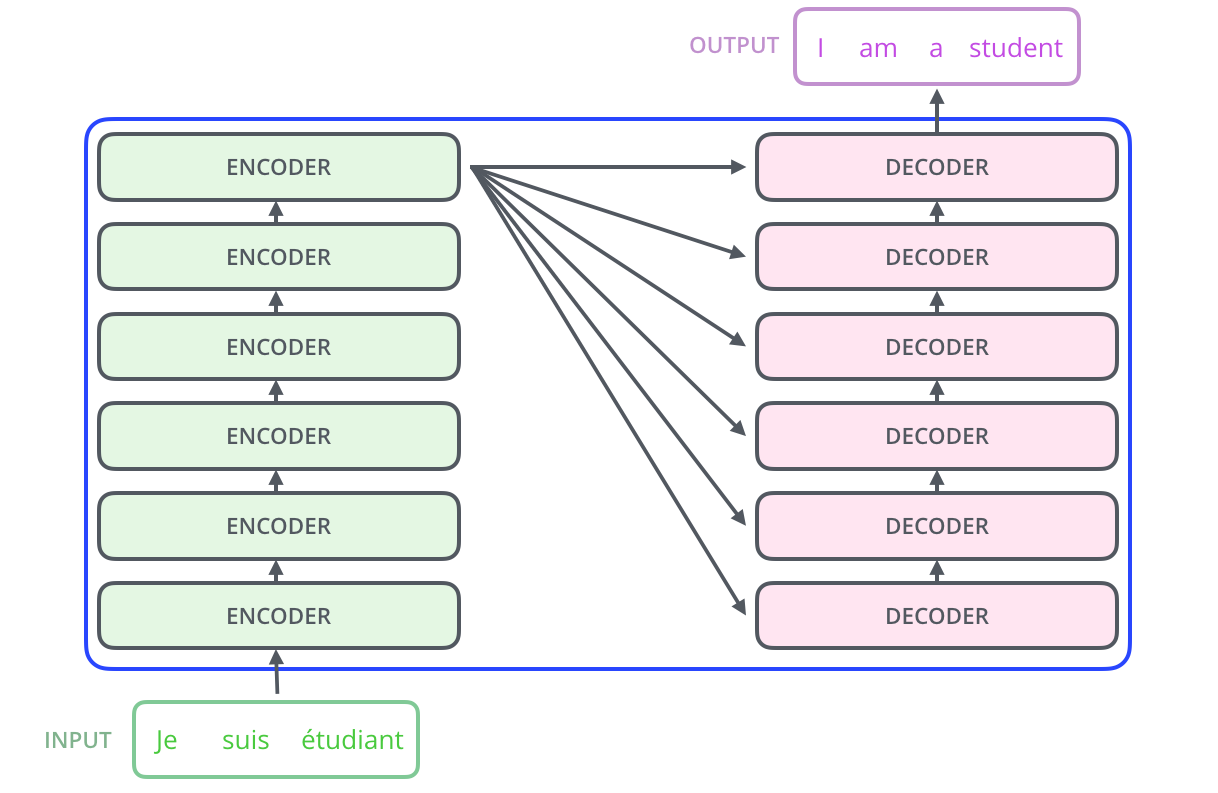
\includegraphics[scale=0.3]{transformer}
	\caption{Visualisierung eines Transformers}
	\label{fig:Transformer}
\end{figure}

\subsection{Generative Adversarial Networks}
\label{sub:gan}
\gls{GAN} verfolgen einen spieltheoretischen Ansatz, im Gegensatz zu einem herkömmlichen
neuronalen Netzwerk. Das Netzwerk erlernt die Generierung aus einer Trainingsverteilung durch ein 2-Spieler-Spiel. Die
beiden Spieler sind der Generator und der Diskriminator. Diese beiden Gegner befinden sich während des gesamten
Trainingsprozesses im ständigen Kampf miteinader. Da eine gegensätzliche (adversielle) Lernmethode angewandt wird,
beinhaltet das Netzwerk einige Eigenheiten.
\newline
\newline
Der Generator wird verwendet um aus einem zufälligen Rauschen möglichst echte Daten zu generieren. Und der Diskriminator
hingegen soll unterscheiden können, ob es sich bei den Daten um echte oder generierte Daten handelt. Die beiden Instanzen
befinden sich im konstanten Kampf gegeneinader, wobei der Generator, versucht möglichst echte Daten zu erzeugen und der
Diskriminator versucht sich nicht täuschen zu lassen. Um möglichst echte Daten zu generieren, benötigt es einen sehr
guten Generator, so wie einen sehr guten Diskriminator. Dies liegt daran, dass wenn der Generator nicht gut genug ist, er
nie in der Lage sein wird, den Diskriminator zu täuschen und das Modell nie konvergieren wird. Wenn aber der
Diskriminator schlecht ist, dann werden auch Bilder, welche keinen Sinn geben, als echt eingestuft. Dadurch kann das
Modell nicht korrekt trainiert werden, denn es gibt keinen genug guten \flqq Validator\frqq \ der Daten.
\newline
\newline
Der Ablauf eines Schrittes in einem \gls{GAN} fängt mit der Erzeugung eines Zufallsrauschens an. Dieses Rauschen wird danach
dem Generator übergegeben, welcher daraus einen möglichst echten Datensatz generiert. Dieser generierte Datensatz wird
anschliessend dem Diskriminator übergeben, welcher entscheidet ob die Daten generiert oder echt sind und gibt demnach
ein entsprechendes Label aus.
\begin{figure}[H]
	\centering
	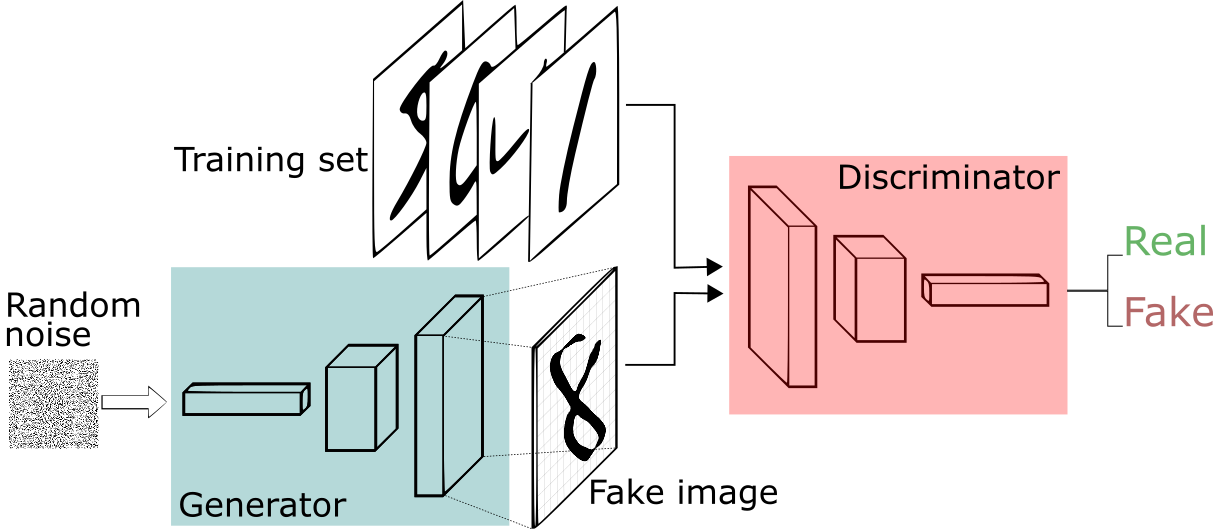
\includegraphics[scale=0.3]{gan}
	\caption{Visualisierung eines GANs}
	\label{fig:GAN}
\end{figure}

\subsection{Aktivierungsfunktionen}
\label{sub:activation-functions}
Aktivierungsfunktionen werden in \gls{NN} gebraucht, um die Ausgaben der einzelnen Layers zu bestimmen. Die
Ausgaben der Layers können mit Ja oder Nein verglichen werden, nur sind es bei den Aktivierungsfunktionen entweder eine
$0$ bis $1$ oder $-1$ bis $1$, je nach Funktion. Aktivierungsfunktionen lassen sich in zwei Typen unterteilen: lineare
Aktivierungsfunktionen und nicht lineare Aktivierungsfunktionen.

\subsubsection{Lineare Aktivierungsfunktionen}
\label{sub:linear-activation}
\begin{figure}[H]
	\centering
	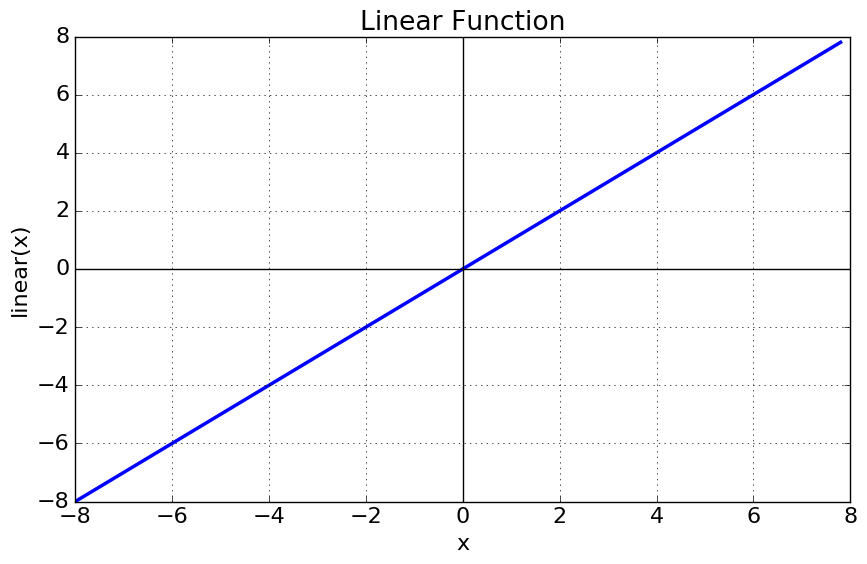
\includegraphics[width=7cm]{Linear_Activation}
	\caption{Lineare Aktivierungsfunktion}
	\label{fig:Linear-Activation}
\end{figure}
\noindent
Bei der linearen Aktivierungsfunktion ist die Funktion eine Linie, die stetig steigt. Daher ist die Ausgabe der Funktion
nicht auf einen Bereich beschränkt. Eine solche Funktion kann zum Beispiel $f(x) = x$ sein, diese befindet sich im
Bereich von $-\infty \ \text{bis} \ \infty$. Das Problem bei linearen Funktionen ist, dass die Daten meist nicht linear
verteilt sind und somit kann sich das Modell nicht genügend den Daten anpassen.

\subsubsection{Nicht lineare Aktivierungsfunktionen}
\label{sub:nonlinear-activation}
\begin{figure}[H]
	\centering
	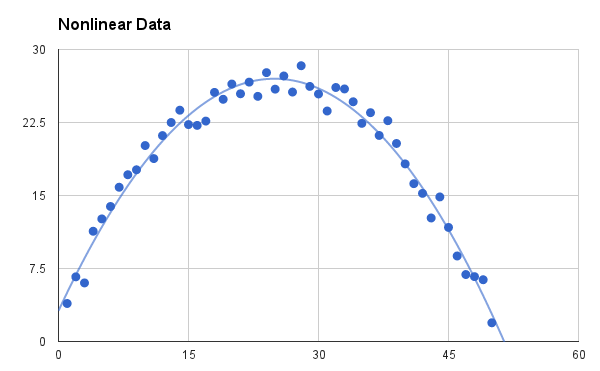
\includegraphics[width=7cm]{Nonlinear_Activation}
	\caption{Nicht lineare Aktivierungsfunktion}
	\label{fig:Nonlinear-Activation}
\end{figure}
\noindent
Nicht lineare Aktivierungsfunktionen werden für die Ausgabe von Layern der neuronalen Netzen am häufigsten verwendet.
Durch die nicht Linearität kann sich das Modell leicht, verschiedensten verteilten Daten anpassen und sehr viele
verschiedene \flqq Formen\frqq annehmen. Eine solche Funktion kann zum Beispiel $f(x) = x^2$ sein.

\subsubsection{Sigmoid}
\label{sub:activation-sigmoid}
\begin{figure}[H]
	\centering
	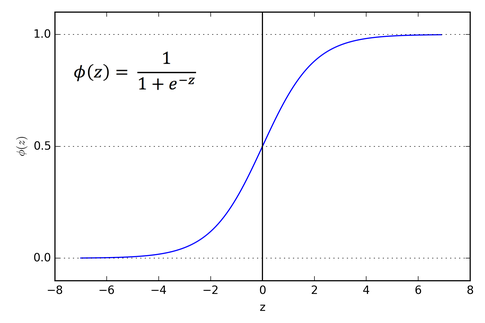
\includegraphics[width=7cm]{Activation_Sigmoid}
	\caption{Sigmoid Funktion}
	\label{fig:Activation-Sigmoid}
\end{figure}
\noindent
Eine Sigmoidfunktion ist eine mathematische Funktion mit einem S-förmigen Graphen, sie ist eine der weitverbreitesten
Funktionen im Umgang mit neuronalen Netzen. Der Grund dafür ist, dass sie sich zwischen $0$ und $1$ befindet. Dadurch
ist die Sigmoidfunktion sehr nützlich an Orten, wo man eine Vorhersage über Wahrscheinlichkeiten treffen muss, da sich
Wahrscheinlichkeiten auch immer zwischen $0$ und $1$ befinden.
\newline
Ein Problem der Sigmoidfunktion ist, dass Parameter \flqq stecken bleiben\frqq \ können, weil sich der Bereich der
Funktion nur zwischen $0$ und $1$ befindet. Somit ist es möglich, dass Parameter die sich sehr nahe bei $0$ befinden nur
wenig angepasst werden und somit gleich bleiben. Dies kann bei Parametern passieren, welche erst nach einer gewissen
Zeit zum Vorschein kommen.

\subsubsection{Tanh}
\label{sub:activation-tanh}
\begin{figure}[H]
	\centering
	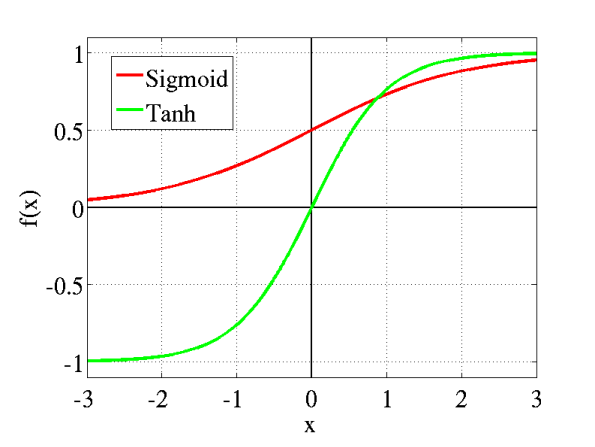
\includegraphics[width=7cm]{Activation_Tanh}
	\caption{Tanh Funktion}
	\label{fig:Activation-Tanh}
\end{figure}
\noindent
Wie die Sigmoidfunktion, ist auch die Tanhfunktion eine mathematische Funktion mit einem S-förmigen Graphen, gibt aber
stattdessen Werte im Bereich von $-1$ und $1$ aus. Somit können stark negative Einträge in der Funktion negativ
abgebildet werden, was in der Sigmoidfunktion nicht möglich ist. Zusätzlich werden nur $0$ ähnliche Einträge auf nahezu
$0$ abgebildet, somit wird das \flqq stecken bleiben\frqq \ beim Training eines Parameters unwahrscheinlicher.
\newline
Die Tanhfunktion wird vor allem bei der Klassifikation von zwei verschiedenen Klassen verwendet.

\subsubsection{ReLU (Rectified Linear Unit)}
\label{sub:activation-relu}
\begin{figure}[H]
	\centering
	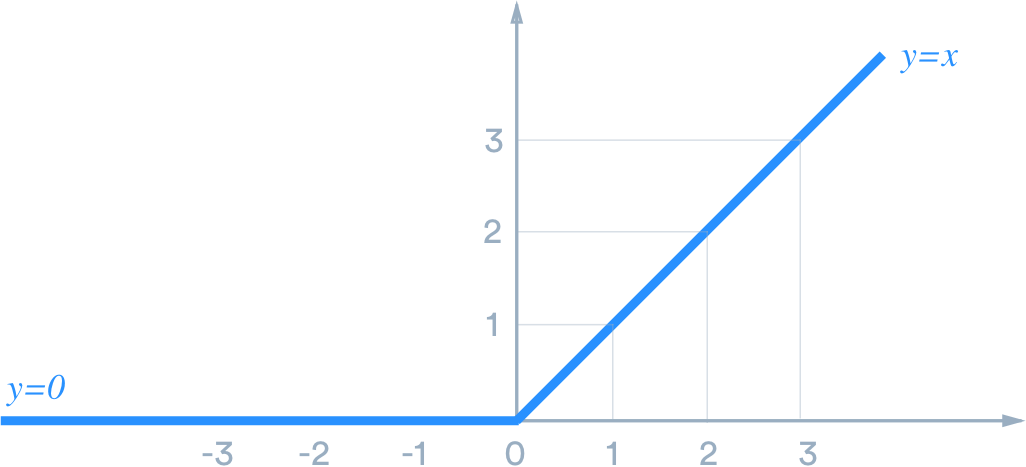
\includegraphics[width=7cm]{Activation_ReLU}
	\caption{ReLU Funktion}
	\label{fig:Activation-Relu}
\end{figure}
\noindent
ReLU ist die am weitesten verbreitete und die am meisten benutzte Aktivierungsfunktion. Sie wird vor allem in
Convolutional Neural Networks sowie in den meisten Deep Learning Modellen gebraucht. Der Bereich der Funktion ist von $0
\ \text{bis} \ \infty$. Ausserdem ist die Funktion, sowie ihre Ableitung monoton.
\newline
Das Problem der ReLU Aktivierungsfunktion ist das Abbilden der negativen Werte, denn jede negative Eingabe der Funktion
wird zu $0$ werden. Dies verringert die Fähigkeit des Modells sich den Daten richtig anzupassen und zu trainieren, denn
die negativen Werte können nicht entsprechend abgebildet werden. Aus diesem Grund wurde die \textbf{Leaky ReLU
Aktivierungsfunktion} entwickelt, welche dieses Problem löst.

\subsection{N-Gramm}
\label{sub:n-gramm}
N-Gramme sind das Ergebnis der Zerlegung eines Textes oder Satzes in einzelne Fragmente. Der Text wird dabei zerlegt und
jeweils $N$ aufeinanderfolgende Fragmente werden als N-Gramme zusammengefasst. Die Fragmente können Buchstaben, Wörter
oder ähnliches sein. Die Zerlegung eines Satzes in N-Gramme wird vor allem zur Hilfe von Analysen oder statistischen
Auswertungen gebraucht.
\newline
Es gibt verschiedene Arten von N-Grammen. Wichtige Arten sind zum Beispiel Monogramme, bei dem $N = 1$, oder Bigramme,
bei dem $N = 2$ ist. Wobei $N$ für die Anzahl Zeichen steht die betrachtet werden.
\newline
\newline
\textbf{Beispiel:}
\begin{align*}
	s (\text{Zeichenkette}) &= \text{\glqq WIPRO\grqq} \\
	N (\text{Anzahl Zeichen}) &= 2\ (\text{Bigramm}) \\
	f (\text{Frequenzwektor}) &= \{\_W:1, WI:1, IP:1, PR:1, RO:1, O\_:1\}
\end{align*}

\subsection{Metriken}
\label{sub:metrics}
Im Bereich von \gls{NLG} sind Metriken ein zentales Thema, da dort ein Vergleich von Labels nicht reicht. Daher mussten
neue Metriken entwickelt werden, die auf den Inhalt der Eingabe und Ausgabe Daten schauen und auf Grund dieses einen
Wertes berechnen wie gut die beiden Daten zusammenpassen. Diese Problematik ist komplex, denn es gibt keinen Blueprint,
der für jeden Fall passt. Eher gibt es einen ganzen Stapel an verschiedenen Methoden zur Auswertung, aus denen eine
entsprechende Metrik gewählt werden muss.
\newline
\newline
Die Intuition für die Bewertung von generiertem Text ist die gleiche wie für die Bewertung von Labels. Wenn der Text $A$
näher an einem der Referenztexte liegt als der Text $B$, dann soll $A$ höher bewertet werden als $B$. Wie bei anderen
Verfahren basiert diese Übereinstimmung auf Präzision (Spezifität, \textit{eng.} specifity) und Erinnerung
(Sensitivität, \textit{eng.} sensitivity). Einfach ausgedrückt, $A$ ist genauer als $B$, falls der Prozentsatz von $A$,
der mit einem Referenztext übereinstimmt, höher ist als $B$. Die Erinnerung von $A$ ist höher, wenn er mehr
übereinstimmenden Text aus einer Referenz enthält als $B$.

\subsubsection{\gls{BLEU}}
\label{sub:BLEU}
\gls{BLEU} ist die weitverbreiteste Metrik für die Bewertung von maschinellen Übersetzungssystemen. Sie wurde im Juli
2002 von einer Forschungsgruppe von IBM entwickelt, da bis dort hin die Metriken zur Auswertung von Machine Translation
zu ineffizient waren. Die Grundsatz Idee von \gls{BLEU} ist: \gls{BLEU} Scores sollen den Unterschied zwischen
Referenzübersetzungen und maschinellen Übersetzungen messen. Dafür werden Präzision und Erinnerung durch modifizierte
n-Gramm-Präzision bzw. beste Abgleichlänge approximiert. 
\newline
\newline
Zunächst werden einzelne Segmente (meist Sätze) verglichen, später wird ein Durchschnittswert für den gesamten Text
ermittelt. Je näher die maschinelle Übersetzung der Referenzübersetzungen kommt, umso besser ist ihr Score. Generell wird
dabei eine Skala von $0$ bis $1$ verwendet, auf welcher der Wert $1$ identisch mit der qualitativ hochwertigen
Referenz-Übersetzung ist, während ein Score von $0$ signalisiert, dass die maschinelle Übersetzung keine
Übereinstimmungen mit der Referenz hat.
\newline
\newline
Ein \gls{BLEU} Score von $1$ ist nicht erstrebenswert, denn dies würde bedeuten, dass die maschinelle Übersetzung
identisch mit der Referenz ist. Dies sollte jedoch in keinem Fall das Ziel sein. Es sollte versucht werden, eine
möglichst korrekte Übersetzung zu liefern und nicht die Referenzübersetzungen zu imitieren.

\paragraph{Interpretation} Es wird dringend davon abgeraten, BLEU-Werte über verschiedene Korpusse und Sprachen hinweg
zu vergleichen. Auch der Vergleich der BLEU-Werte für denselben Korpus, aber mit einer abweichenden Anzahl von
Referenzübersetzungen, kann sehr irreführend sein. Die genauere Interpretation des Wertes ist in Tabelle
\ref{tab:BLEU-Interpretation} ersichtlich.

\begin{table}[ht]
	\begin{tabular}{| c | l |}
	\hline
	BLEU-Wert            & Interpretation                                                            \\ \hline
	\textless \ 0.1      & Fast unbrauchbar                                                          \\
	0.1 – 0.2            & Schwierig, das Wesentliche zu verstehen                                   \\
	0.2 – 0.3            & Das Wesentliche ist verständlich, aber es gibt erhebliche Grammatikfehler \\
	0.3 – 0.4            & Verständliche bis gute Übersetzungen                                      \\
	0.4 – 0.5            & Hochwertige Übersetzungen                                                 \\
	0.5 – 0.6            & Sehr hochwertige, adäquate und flüssige Übersetzungen                     \\
	\textgreater \ 0.6   & Qualität oft besser als menschliche Übersetzungen 					     \\
	\hline                        
	\end{tabular}
	\caption{Interpretation des BLEU Wertes}
	\label{tab:BLEU-Interpretation}
\end{table}

\paragraph{Mathematischen Details}
Mathematisch wird der BLEU-Score definiert mit ~\autocite{modelle_bewerten_bleu}:

\begin{equation}
	\text{BLEU} = \underbrace{\vphantom{\prod_i^4}\min\Big(1,\exp\big(1-\frac{\text{reference-length}}{\text{output-length}}\big)\Big)}_{\text{brevity penalty}}
\underbrace{\Big(\prod_{n=1}^{4}
\text{precision}_n\Big)^{1/4}}_{\text{n-gram overlap}}
\end{equation}
\myequations{BLEU Score}
mit
\begin{equation}
	\text{precision}_n = \dfrac{\sum_{\text{sentence}\in\text{Candidates-Corpus}}\sum_{n\in\text{sentence}}\min(m^n_{cand}, m^n_{ref})}
{w_t^n = \sum_{\text{sentence'}\in\text{Candidates-Corpus}}\sum_{n'\in\text{sentence'}} m^{n'}_{cand}}
\end{equation}
\myequations{Precision im BLEU Score}
wobei $n$ die Anzahl an \textit{n-grams} ist.
\newline
\newline
Wobei Folgendes gilt:
\begin{itemize}
	\setlength\itemsep{0em}
	\item $m^n_{cand}$ entspricht der Anzahl an n-Gramme für den Kandidaten, die mit der Referenzübersetzung
	übereinstimmen
	\item $m^n_{ref}$ entspricht der Anzahl an n-Gramme in der Referenzübersetzung
	\item $w^i_t$ entspricht der Gesamtzahl der n-Gramme in der Kandidatenübersetzung
\end{itemize}
Die Formel besteht aus zwei Teilen: dem Abzug für die Kürze (\textit{eng.} brevity penalty) und der N-Gramm
Übereinstimmung (\textit{eng.} n-gram overlap).
\begin{itemize}
	\setlength\itemsep{0em}
	\item Der Abzug für die Kürze bestraft generierte Übersetzungen, die verglichen mit der ähnlichsten Referenzlänge
	exponentiell abnehmend zu kurz sind. Dies kompensiert den fehlenden Trefferquoten (\textit{eng.} recall) Term.
	\item Die N-Gramm-Übereinstimmung zählt, wie viele N-Gramme mit ihrem N-Gramm-Gegenstück in den
	Referenzübersetzungen übereinstimmen. Über die N-Gramm-Übereinstimmung wird die Genauigkeit (\textit{eng.}
	precision) der Übersetzung gemessen. Kürzere N-Gramme ermitteln die Ädequatheit, längere N-Gramme die Flüssigkeit
	der Übersetzung. Zur Vermeidung einer unnötigen Zählung wird die N-Gramm-Zählung auf die maximale N-Gramm-Anzahl
	begrenzt, die in der Referenz auftritt ($m_{ref}^n$).
\end{itemize}

\subsubsection{\gls{TER}}
\label{sub:TER}
Während es bei \gls{BLEU} vor allem darum geht, zu bestimmen, wie nah eine maschinelle Übersetzung einer Referenz kommt,
sagt \gls{TER} aus, wie viele Schritte im Post-Editing benötigt werden, um von der erstellten maschinellen Übersetzung
zur korrekten Übersetzung zu gelangen. \gls{BLEU} und \gls{TER} sind sich in vielerlei Hinsicht sehr ähnlich und werden
daher gerne zusammen verwendet.
\newline
\gls{TER} wie auch \gls{BLEU}, interessieren sich nicht für die zu grunde liegende Sprache des Satzes, sonden der
Algorithmus möchte nur herausfinden, wie viele Unterschiede es zwischen dem Referenzsatz und dem generierten Satz gibt.
\newline
Auch \gls{TER} benötigt einen Referenzkorpus an dem gemessen werden soll, wie nahe der generierte Output der Referenz
kommt.
\newline
Diese Metrik wird dazu verwendet um zu prüfen, wie viele verändernde Schritte nötig sind um ein gutes Ergebnis zu
erhalten.
\begin{equation}
	\text{TER} = \frac{\text{\# of edits}}{\text{average \# of references}}
\end{equation}
\myequations{TER Score}

\section{Stand im Bezug auf eigenes Projekt}
\label{sec:stand-bezug-projekt}
Alle erwähnten technischen Konzepte sind längst keine eigenständigen, geschlossenen Einheiten mehr. Sondern werden in
den aktuellen Forschungen miteinader verknüpft und es werden vielversprechende Ansätze von einem Konzept ins Andere
übernommen, um neue Architekturen für verschiedene Probleme zu entwickeln. Auf diese Art und Weise sind die meisten
Durchbrüche der aktuellen Forschung gelungen.
\newline
\newline
Eines der aktuellsten Themen im Bereich von \fullref{sub:natural-language-generation} und
\fullref{sub:natural-language-processing} ist \fullref{sub:neural-style-transfer}, welches in momentanen Forschungen auf
Textbasierte Daten angewendet wird, mit moderaten Ergebnissen, um den Stil eines Satzes auf einen anderen zu übertragen.
Bei diesem Ansatz werden meist \fullref{sub:rnn}, \fullref{sub:lstm}, \fullref{sub:autoencoder} und viele weiter der
oben erwähnten Konzepte verwendet.


\chapter{Ideen und Konzepte}
\label{ch:ideen_konzepte}
In diesem Kapitel werden auf die verschiedenen Ideen und Konzepte genauer eingegangen, welche in der Arbeit verwendet
wurden. Es beinhaltet Ideen zu dem verwendeten Datensatz, den verwendeten Modellen und dem Training der Modelle.

\section{Problemdefinition}
\label{sec:Problemdefinition}
Der Aufbau eines Satzes $ S $ kann linguistisch als Semantik und Syntax beschrieben werden.
\noindent
\myequations{Struktur eines Satzes}
\begin{equation}
	S = S_{semantic} + S_{syntax}
	\label{eq:structure_sentence}
\end{equation}
\noindent
Syntax und Semantik in der natürlichen Sprache zu trennen, ist eine Herausforderung. Da vor allem das Erkennen der
Semantik schwierig ist, denn die selben Wörter in unterschiedlichen Kontexten können zur Syntax oder auch zur Semantik
gehören. Zu beachten ist, dass die Syntax einen Einfluss auf die Semantik haben kann. So zum Beispiel das Pronomen \flqq
nichts\frqq \ und das gross geschriebene Substantiv \flqq Nichts\frqq. So kann der Transfer, welcher \flqq positive\frqq
in \flqq negative\frqq \ Sätze wandelt, die Semantik des Ausgabesatzes beeinflussen. Jedoch möglichst den Bezug zum
Kontext, dem positiven oder negativen Subjekt, zu wahren.
\newline
\newline
Der Input des zu erarbeitenden Prototypen des Zeugnismanagers, ist die Bewertung $ c_{P} $ einer Person $ P $ sowie eine
Eingabesequenz $x$. Diese Bewertung $c_P$ ist dem Kontext eines Satzes gleich zu stellen, und soll beim Transfer nicht
geändert werden. Ausserdem wird jeder Satz einem stylistischen Label $y$ zugeordnet. Aus der Bewertung, Stylelabel und dem
Eingabesatz folgt $ x $ welcher aus $c_P$ und $y$ zusammengesetzt ist, ähnlich wie \ref{eq:structure_sentence}.
\noindent
\myequations{Möglichkeiten der Werte der Stillabels}
\begin{equation}
	\begin{split}
		y_k = holprig &= klexikon \\
		&\text{oder} \\
		y_w = flüssig &= wikipedia
	\end{split}
	\label{eq:style_labels}
\end{equation}
\noindent
Diese Labels sind wie in Formel \ref{eq:style_labels} ersichtlich, in $holprig$ und $flüssig$ unterteilt. Dabei soll
$holprig$ bedeuten, dass der Satz aus dem Zeugnismanager generiert wurde und noch gewisse Verbesserungen vorgenommen
werden müssen bevor dieser in ein Arbeitszeugnis einfliessen kann. $flüssig$ hingegen bedeutet, dass die Sequenz
qualitativ hochwertig ist und nicht mehr weiter bearbeitet werden muss. Diesen definierten Labels wurden, aufgrund der
\fullref{sec:abschliessende_problemdefinition} ein synonymes Label zugeordnet, welches den Datensatz
\ref{sec:verwendeter_datensatz} wiederspiegelt. Aus der Anforderung folgt, dass der angestrebte Zielstil $y_w$ ist.
\newline
\newline
Wie aus der \fullref{sub:aufgabenstellung} zu entnehmen ist, entspricht der Stil der Eingabesatzes $x$ dem Stillabel
$y_k$ und soll in den Zielstil $y_w$ transferiert werden, ohne dass dessen Bewertung $c_P$ verloren geht. Somit entsteht
ein neuer transferierter Satz $\hat{x}$.
\myequations{Aufgabenstellung mathematisch formuliert}
\begin{equation}
	\hat{x} = (x - y_k)  + y_w \quad mit \quad y = y_w
	\label{eq:problemdefinition}
\end{equation}

\section{Abschliessende Problemdefinition}
\label{sec:abschliessende_problemdefinition}
Ein Wissenstext für Kinder aus dem Klexikon, unterscheidet sich im Schreibstil zu einem Text für Erwachsene aus
Wikipeida. Durch das Ersetzen von $ holprig $ und $ flüssig $, durch $ klexikon $ und $ wikipedia $ kann ein ähnliches
Problem, wie in \fullref{sec:Problemdefinition} beschrieben, modelliert werden. Wie unter
\fullref{sub:statistische_analyse_des_datensatz} aufgezeigt, beinhalten die Sätze von Wikipedia, Stillabel $ wikipedia
$, mehr Wörter als die Sätze aus dem Klexikon, mit Stillabel $ klexikon $. Daher kann das Problem abschliessend so
beschreiben werden, dass der Style Transfer aus einem kurzen Satz einen längeren Satz mit gleichem, erweiterten Inhalt
generiert. Ensprechendes gilt für den umgekehrten Fall. So sollte die Länge der generierten Sätze aus einem Stillabel
der Verteilung der Länge aus dem Zielstil folgen.

\section{Verwendeter Datensatz}
\label{sec:verwendeter_datensatz}
Um die mögliche Modelle evaluieren zu können, wird ein Datensatz aufbereitet. Für die Gebiete von Arbeitszeugnisse sind
leider zu wenig Daten vorhanden. Eine naheliegende Möglichkeit ist, die Daten eines Lexikon oder andere, weitverbreitete
und vielfach übersetzte Informationen. Die Texte weisen dabei einen zielgruppengerechten Schreibstil auf.
\newline
\newline
Themengebiete aus welchem entsprechende Texte stammen könnten sein,
\begin{enumerate}
	\setlength\itemsep{0em}
	\item Lexikon / Wikiseite
	\item Bibel
	\item Zeitungen
\end{enumerate}
\noindent
Bei der Recherche für eine geeignete Datenquelle, wurden Zeitungen früh ausgeschlossen. Es finden sich keine
praktikablen und einfach zusammentragbaren Kinderzeitungen online. Weiter wären die Themen der Zeitungsartikel sehr
breit aufgestellt. Auch fokussieren sich Kinderzeitungen nicht auf das gleiche Weltgeschehen wie Zeitungen.
\newline
\newline
Aus dem Themengebiet der Religion, namentlich \flqq die Bibel\frqq, finden sich zahlreiche Quellen. Dabei unterscheidet
sich jedoch der Inhalt teilweise enorm. Hierzu werden in Kinderbibeln oft eine vielzahl an Illustrationen verwendet.
Auch sind sie oft als Erzählbücher gestaltet. So unterscheiden sie sich nicht zwingend im Schreibstil, jedoch mehr in
der Wortwahl. Weiter fanden sich wenige Quellen, bei welchen die Daten in einem handhabaren Format aufbereitet sind.
Eine Extraktion der Texte aus PDFs oder gar gebundenen Bücher hätte einen zu grossen Aufwand mit sich gezogen. Daher
wurde die Verwendung der Bibel als Quelle bis auf weiteres zurückgestellt.
\newline
\newline
An Lexikas gibt es eine Vielzahl von Ausgaben. Sowohl für Erwachsene als auch für Kinder. Die naheliegenste Quelle für
Texte für Fortgeschrittene ist, die Online Enzyklopädie \flqq Wikipedia\frqq. Bei der Recherche liess sich ebenfalls ein
Online Lexikon für Kinder finden, das \flqq Klexikon\frqq. Diese beiden Quellen basieren auf dem Open-Source Framework
\flqq WikiMedia\frqq. Entsprechend kann einfach ein Crawler für diese Seiten erstellt werden. Das Klexikon enthält ca.
2'700 Artikel, in einem für Kinder verständlichen Schreibstil. Für nahezu alle Artikel besteht ein korrespondierender
Artikel in Wikipedia. Nach Rücksprache mit der Betreuungsperson hat man sich für die Verwendung dieser Artikel
entschieden. Die Aufbereitung des Datensatzes wird im Kapitel \fullref{ch:Realisierung} beschrieben.

\section{Momentan verfügbare Forschung}
In einem ersten Teil wurde nach bestehenden Forschungen, im Bereich der Problemstellung, gesucht. Es konnten schnell
viele verschiedene Ansätze gefunden werden, um das Problem lösen zu können. Dabei gab es viele unterschiedlichen
Lösungsansätzen, \gls{NST}, \gls{RNN}, Transformer, Fuzzy Logic und noch viele weitere. Es wurde schnell klar, dass das
Gebiet eingeschränkt werden muss, um die Ressourcen des Projektes optimal auszuschöpfen. Das spannendste Teilgebiet war
der \gls{NST}, auf welches sich diese Forschung hauptsächlich konzentrierte.
\newline
\newline
Bei der Suche nach den vielversprechendsten Ansätzen von \gls{NST}, wurden eine Menge an aktuellen Forschungen gefunden,
da das Gebiet als ehr jung gilt. Die meisten dieser Arbeiten fokussieren sich auf die Übertragung von der Stimmungslage
in eine andere, zum Beispiel von einem positiven in einen negativen Satz. Diese Problemdefinition wird im \gls{NST}
immer wieder verwendet um neue Modelle zu testen. Meistens werden dafür Sätze von Bewertungen (z.B. Tripadvisor oder
IMDB) als Datensatz verwendet. Diese Problemstellung dient in den meisten Fällen nur zur Veranschaulichung der
Einsatzmöglichkeiten der Modelle.
\newline
\newline
Bei der Recherche wurde ein sehr gut gepflegtes und aktuelles GitHub Projekt gefunden, welches sich darauf fokussiert,
die neusten wissenschaftlichen Arbeiten, im Gebiet des Style Transfer, zu verlinken. Ausserdem wird immer versucht Code
zu den entsprechenden Werken zu finden und zu verlinken. Das Repository findet sich auf GitHub unter
\hyperlink{https://github.com/fuzhenxin/Style-Transfer-in-Text}{GitHub Style Transfer in Text}
(\cite{fuzhenxin_style_transfer_in_text}).
\newline
Im Projekt werden die Arbeiten in verschiedene Abschnitte unterteilt, je nach dem, um welches Untergebiet es sich
handelt: Dataset, Supervised (Parallel Data), Unsupervised (Non-parallel Data) und Semi-Supervised. Es wurde sehr
schnell klar, dass die Unterlagen im Bereich Supervised und Semi-Supervised nicht erforscht werden müssen, da es sich
bei unserem Datensatz \ref{sec:verwendeter_datensatz} um nicht parallele Daten handelt.
\newline
Im Bereich des Unsupervised Style Transfer, wurden verschiedene Arbeiten, im Bezug auf die Anwendbarkeit auf unsere
Problemdefinition, untersucht. Dabei wurden vor allem die Unterlagen mit entsprechendem Code untersucht, da die
Umsetzung solcher Arbeiten sehr aufwendig ist. Die meisten dieser Papers beschreiben ein spezielles Modell, welches
einen Style Transfer für bestimmte Probleme vornehmen kann. Diese Modelle sind meistens sehr ähnlich aufgebaut und haben
viele Gemeinsamkeiten. Notizen zu den einzelnen Arbeiten kann im Anhang unter \fullref{app:recherche} gefunden werden.
\newline
\newline
Es wurde schnell bemerkt, dass viele der untersuchten Arbeiten immer wieder die Modelle \textbf{ControlGen} und
\textbf{CrossAlign} brauchen um neue exotische Architekturen zu überprüfen, meistens mit der Frage: \glqq Ist die neue
Architektur besser als die allgegenwärtige?\grqq Daher wurde sehr schnell klar, das in diesem Projekt diese Baseline
Modelle verwendet werden sollen, da es sich bei dem Problem um erste Versuche mit \gls{NST} in deutscher Sprache
handelt. Weitere Architekturen können in einem weiterführenden Projekt untersucht werden, übersteigen jedoch den Rahmen
dieses Projektes.
\newline
\newline
Anschliessend wurden die Unterlagen zum ControlGen (\cite{hu2017controlled}) und CrossAlign (\cite{shen2017style})
Modell durchgearbeitet. Beide Arbeiten der Modelle haben auch eine Implementation in Tensorflow, diese wurden auch genau
untersucht, um die Architekturen besser zu verstehen. Sehr schnell wurde bemerkt, dass die Standardimplementationen der
Modelle eher dürftig sind und es wurde weiter gesucht, nach besseren Implementationen.
\newline
Im Repository wurde dann das Paper (\cite{Li2019DomainAT}) gefunden, welches die beiden Architekturen als Baseline
brauchen um ihre domain adaptiven Modelle damit zu vergleichen. Die Arbeit möchte vor allem zeigen, dass es mit ihren
Modellen möglich ist, durch parallele Daten nicht nur den Stil zu erlernen, sondern auch deren Domäne und ihre
Eigenschaften. Die Idee des Projektes ist sehr interessant, jedoch können diese speziellen Modelle nicht auf unseren
Datenkorpus angewendet werde. Das Projekt bietet aber einen hochwertigen Implementation in Python und Tensorflow zu den
beiden Modellen. Daher wurde entschieden dieses Projekt für die Experimente und das weitere Projekt zu verwenden. Das
Original Repository findet sich auf GitHub unter \hyperlink{https://github.com/cookielee77/DAST}{GitHub DAST}
(\cite{cookielee77_dast}).

\subsection{Modelle}
\label{sub:modelle}
Das Repository (\cite{cookielee77_dast}) welches in diesem Projekt verwendet wurde, beinhaltet zwei Style Transfer
Modelle, \fullref{sub:control_gen} und \fullref{sub:cross_align}. Diese beiden sind im Grundsatz sehr ähnlich und erben
daher beide vom \fullref{sub:base_model}, daher können die Modelle gleich trainiert, getestet und verwendet werden.
Ausserdem sind die Hyperparameter der beiden Architekturen identisch und können somit gegenüber gestellt werden. Um die
beiden Modelle zu evaluieren, befindet sich in dem Projekt ein \fullref{sub:classifier}. Dieser ist dafür zuständig, zu
überprüfen ob die Sätze zu dem korrekten Style transferiert wurden. Mittels dem Classifier kann daher eine
\textit{transfer accuracy} berechnet werden.
\begin{figure}[H]
	\centering
	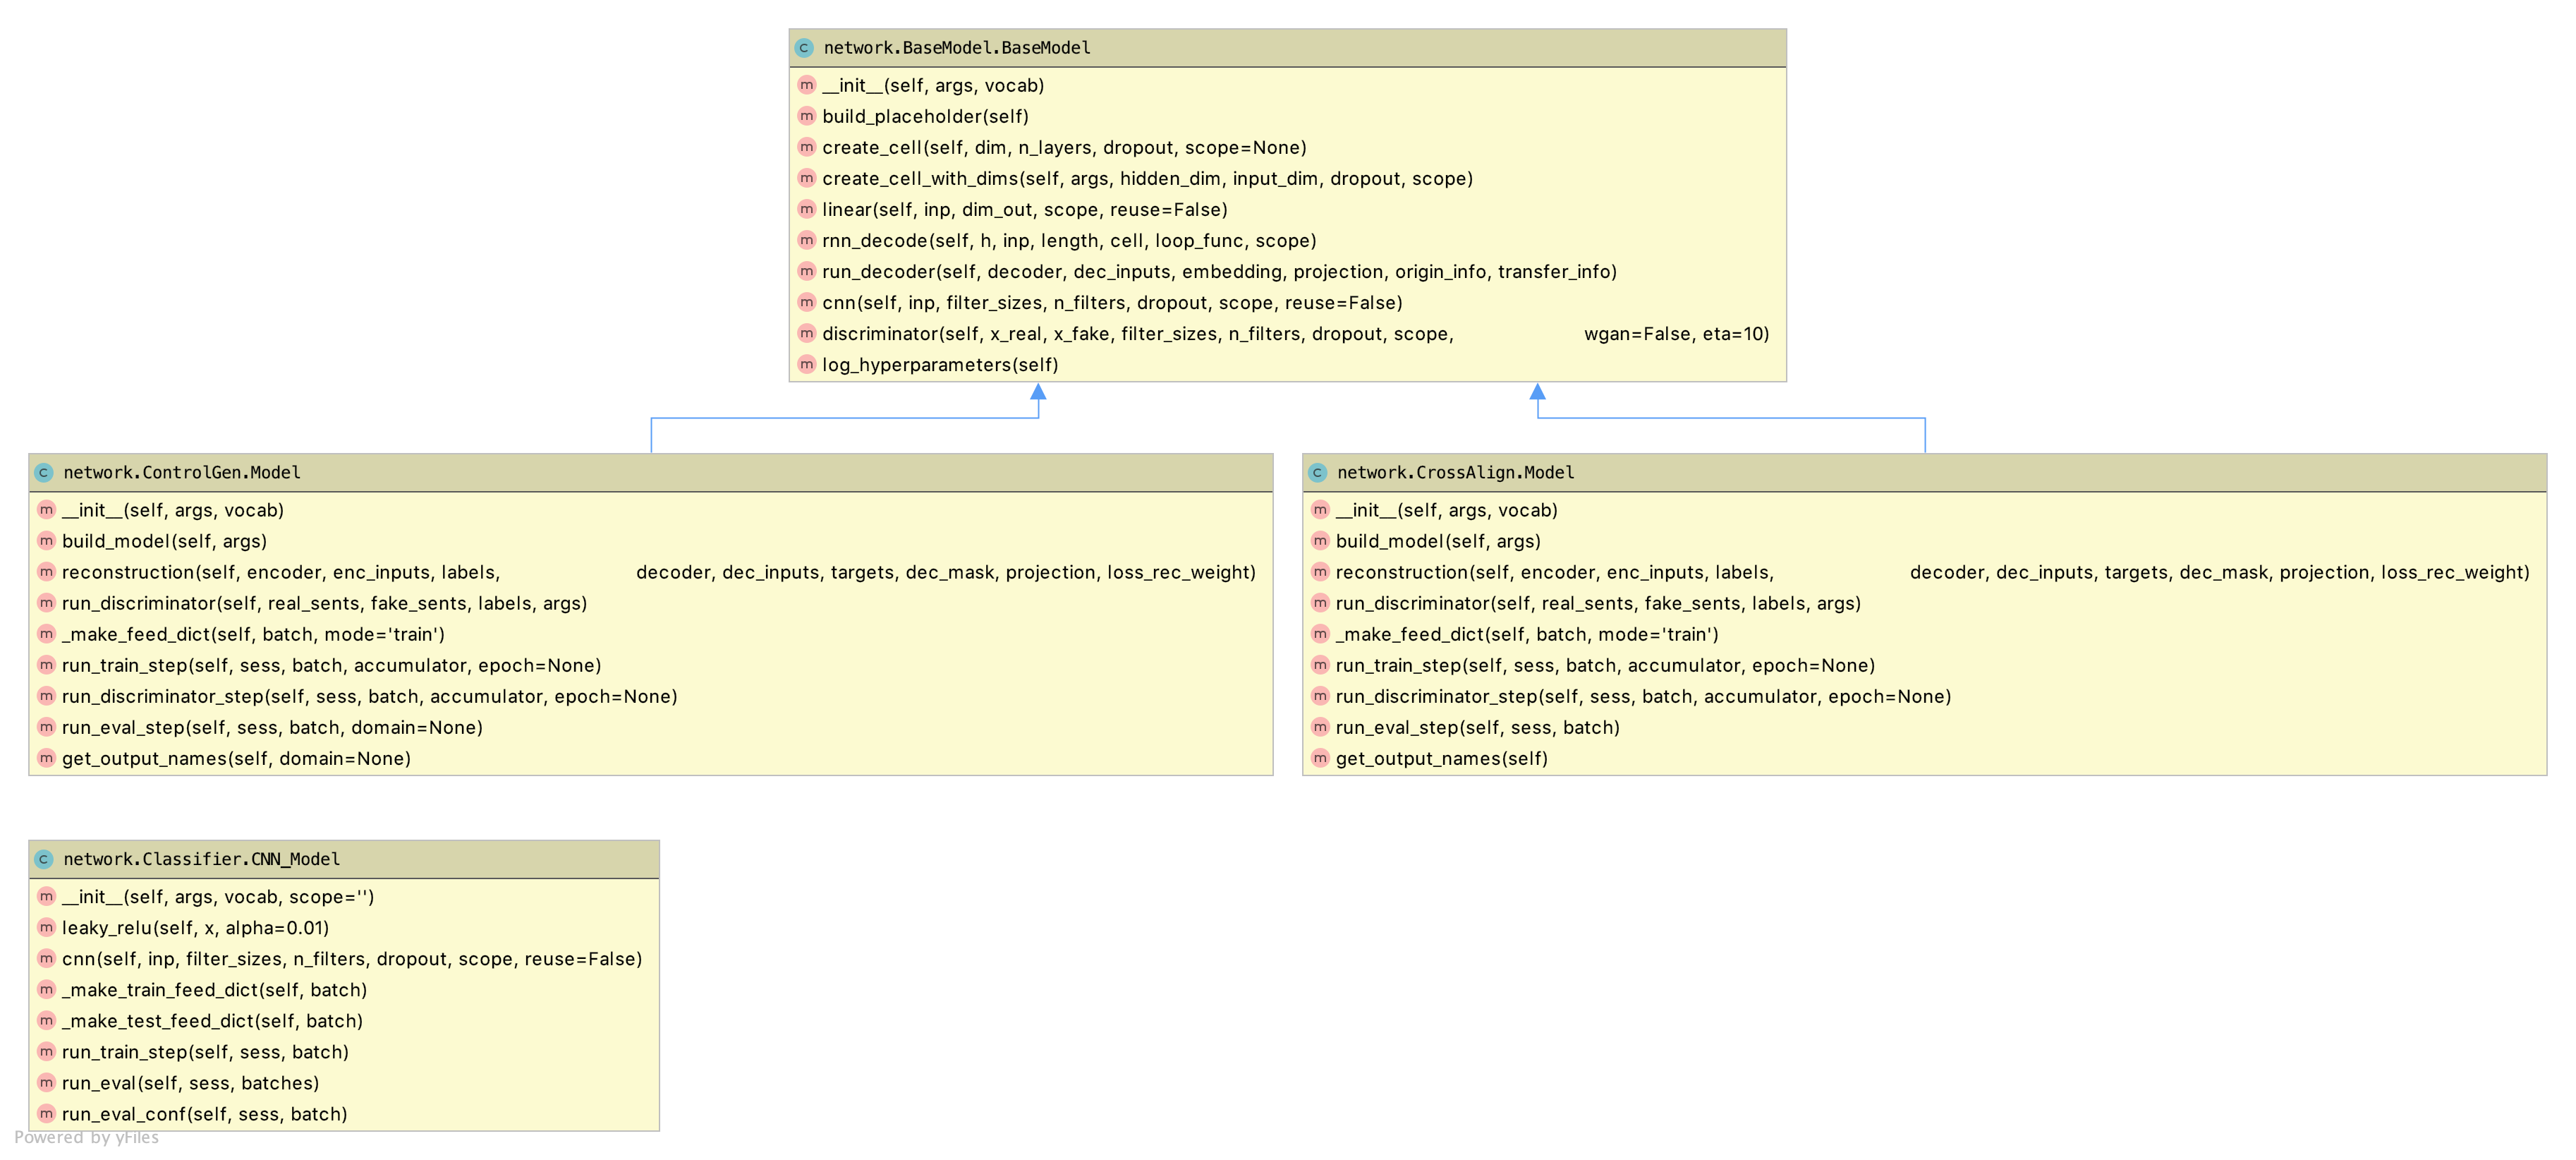
\includegraphics[scale=0.11]{uml_models}
	\caption{Klassendiagramm der Modelle}
	\label{fig:uml_models}
\end{figure}
\noindent
Die Modelle wurden mit dem Datensatz, welcher in \fullref{sec:verwendeter_datensatz} beschrieben wurde, trainiert und
evaluiert. Um diesen Datensatz für das Modell lesbar zu machen, müssen die Sätze in einen Vektor aus IDs transformiert
werden. Jede ID repräsentiert dabei ein Wort, und kann damit eindeutig zugeordnet werden. 
\newline
\newline
Um diese Vektoren zu erstellen, muss als erstes ein Vokabular von den Daten erstellt werden. Dieses beinhaltet alle
Vorkommnisse der einzelnen Wörter im Datenkorpus. Um die Grösse dieses Vokabulars einzuschränken, muss jedes Wort eine
gewisse Anzahl darin vorkommen um aufgenommen zu werden, diese Anzahl an Vorkommnissen ist als
Hyperparameter verfügbar. 
\newline
\newline
Jedem dieser Wörter im Vokabular wird eine eindeutige ID zugeordnet um ein \flqq Wort zu ID\frqq \ und \flqq ID zu
Wort\frqq \ Array zu erstellen. Diese beiden Arrays werden danach genutzt um die einzelnen Sätze in ID Vektoren zu
transformieren und wieder zurück. Wenn nun ein Wort, welches das minimale Vorkommen im Datenkorpus nicht erreicht hat,
transferiert werden möchte, wird diesem Wort ein Platzhalters zugeordnet, wie zum Beispiel \verb|<unk>|. Dadurch kann es
sein, dass bei der Rekonstruktion der Sätze aus den ID Vektoren solche Platzhalter vorkommen, was in
\fullref{sec:eval_output} ersichtlich ist.

\subsection{Classifier}
\label{sub:classifier}
Der Classifier ist ein \gls{CNN}, welches aus mehreren Schichten mit dem gleichen Aufbau bestehen. Zuerst eine
convolution Schicht gefolgt von der Leaky Relu Aktivierungsfunktion \ref{sub:activation-relu} und zum Schluss noch ein
Max-Pooling Layer. Dieser Aufbau wird mehrmals hintereinander geschaltet. Als Verlustfunktion wird eine Softmax Funktion
verwendet, da es sich bei den Daten um gelabelte Daten, welche entweder $0$ oder $1$ sind, handelt. Als Optimizer wird
hier und im ganzem Projekt Adam verwendet. Das Ziel des Classifiers ist es ein \gls{CNN} zu trainieren um zu
unterscheiden ob es sich bei dem vorliegenden Satz um einen Klexikon oder Wikipedia Satz handelt.
\begin{figure}[H]
	\centering
	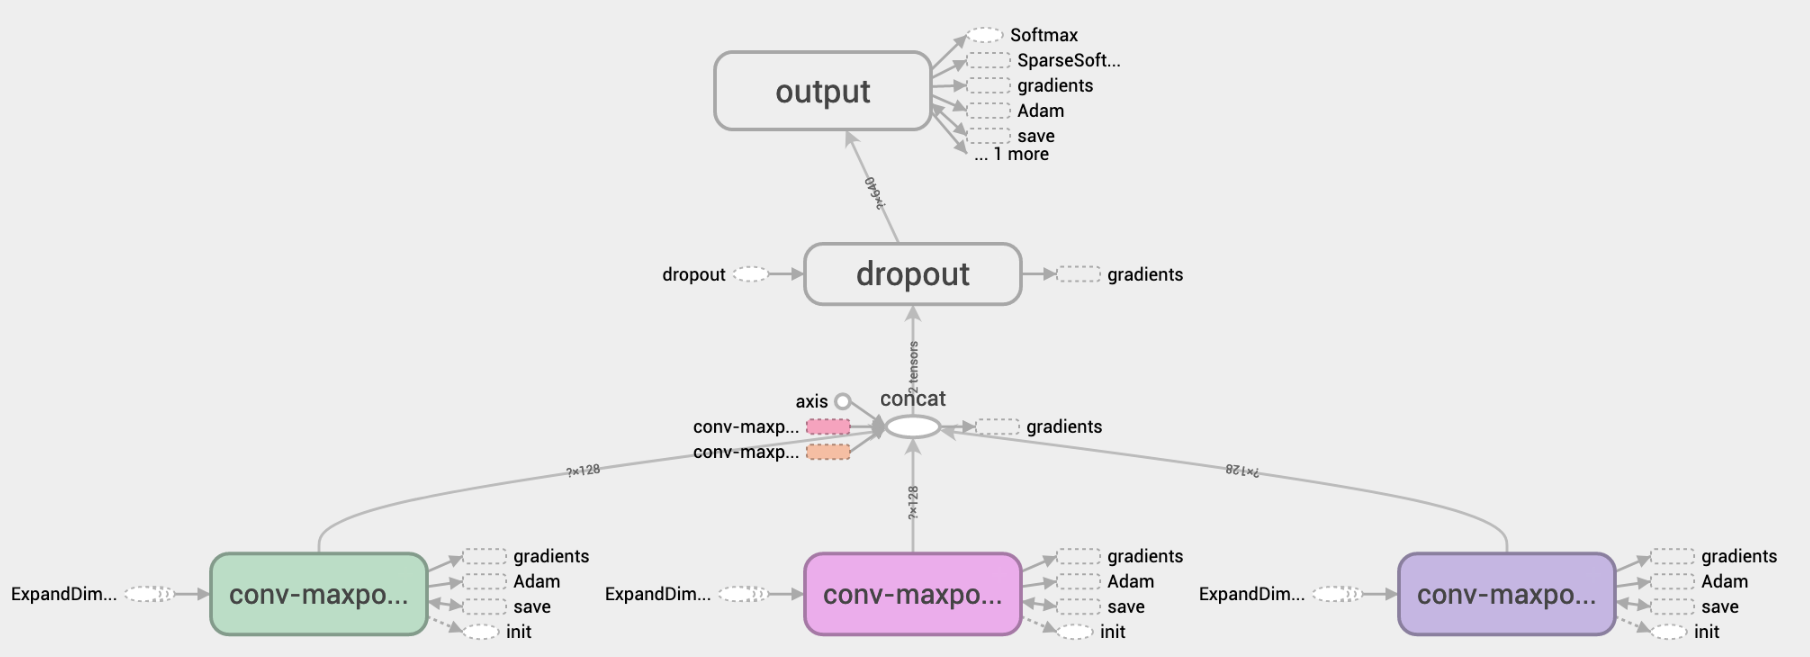
\includegraphics[scale=0.425]{classifier_architecture}
	\caption{Visualisierung der Classifier Architektur}
	\label{fig:classifier_architecture}
\end{figure}
\noindent
Beim Classifier können mit verschiedenen Hyperparameterern unterschiedliche Ergebnisse erzielt werden, je nachdem wie
der Datenkorpus aufgebaut ist und von welcher Grösse dieser ist.
\begin{table}[ht]
	\centering
	\begin{tabular}{| l | l |}
	\hline
	\textbf{Hyperparameter} & \textbf{Interpretation}                                     \\ \hline
	learning rate           & Wie stark die Funktion sich in die Richtung des             \\ 
	                        & Minimums bewegen soll                                       \\ \hline
	dimension embedding     & Dimension des verwendeten Embedding Layers                  \\ \hline
	filter sizes            & Wie gross die einzelnen Filterkernels der Layers sind       \\ \hline
	number of filters       & Anzahl der Filters pro Convolution Schicht                  \\ \hline                     
	\end{tabular}
	\caption{Hyperparameter des Classifiers}
	\label{tab:Hyperparameter_classifier}
\end{table}

\subsection{BaseModel}
\label{sub:base_model}
Das BaseModel wird in beiden Architektur \fullref{sub:control_gen} und \fullref{sub:cross_align} verwendet, um ein
objektorientierter Ansatz zu verfolgen. Dieses Modell ist nicht vollständig und kann nicht ohne weitere Implementationen
trainiert werden, es dient nur der Abstraktion. In diesem Modell werden alle Hyperparameter für die geerbten Modelle zur
Verfügung gestellt, sowie die wichtigsten Variablen definiert, Dropout, Batch Länge, Encoder Inputs, Decoder Inputs und
noch viele weitere. Ausserdem beinhaltet das Base Modell Implementationen zu den wichtigsten Bestandteile der Netwerke.
Wie zum Beispiel die Implementation einer einzelnen \gls{RNN} Zelle, einer linearen Funktion, einem \gls{CNN} und dem
Diskriminator des \gls{GAN}. Durch das Modell ist es möglich, die verwendeten Hyperparameter der Modelle in einem
lesbaren Format zu loggen.

\subsection{ControlGen}
\label{sub:control_gen}
Das ControlGen Paper (\cite{hu2017controlled}) schlägt ein neues generatives Modell vor, welches \gls{VAE} und Ansätze
eines \gls{GAN} kombiniert um die effektiven semantischen Strukturen von Daten zu erlernen. Mit dieser Kombination soll
das Modell im Stande sein Sätze zu interpretieren und diese mit den gewünschten Eigenschaften zu transformieren. Dabei
soll ein besonderes Augenmerk darauf gelegt werden, dass die Erzeugung der Sätze mittels Merkmale kontrolliert werden
kann.
\newline
\newline
Das Modell zielt darauf ab, plausible Sätze zu erzeugen, die auf Repräsentationsvektoren basieren, die aus bestimmten
semantischen Strukturen aufgebaut sind. Für die Kontrolle des Satzstiles, wird das Modell eine Dimension des
Latentcodes, für den $klexikon$ und $wikipedia$ Stil, zugewiesen. Das Erzeugen des entsprechenden Stils, geschieht
aufgrund der Angabe des entsprechenden Latentcodes. Eine solche Dimension, erfasst immer ein markantes Attribut der
Daten, welches von anderen Merkmalen unabhängig ist.
\newline
\newline
Die ControlGen Architektur baut auf der Struktur eines \gls{VAE} auf, welches aus einem traditionellem Auto-Encoder
besteht, wobei der Latentspace regularisiert wird, um kontrolliert Daten zu erzeugen. Der Encoder des Modelles bekommt
als Input eine Textsequenz $x$, diese wird auf den Latentspace $z$ projiziert, welche die einzelnen Latentcodes $c$ als
Dimensionen enthalten. Die Abbildungen des Inputs auf den Latenspace $z$ sind unstrukturierte Vektoren, welche
reduzierte wichtige Merkmale eines Satzes beinhalten, um diesen wiederherzustellen. Um diese Attribute besser abzubilden
und zu kontrollieren, wird der Latentspace $z$ um eine Reihe von strukturierten Variablen $y$, den Latentcodes, ergänzt,
von denen jede auf ein markantes und unabhängiges semantisches Merkmal abzielt, den Labels der Daten. Diese Latentcodes
$y$ werden im Netzwerk manipuliert um Daten im gewünschten Label zu erzeugen. Der Generator soll von dem kombinierten
Vektor $z$ und $y$ abhängig sein, und generiert Daten welche die semantischen Merkmale des strukturierten Codes $y$
erfüllen. Dieser grobe Ablauf des Modelles ist in Abbildung \ref{fig:control_gen_overview} anschaulich dargestellt.
\begin{figure}[H]
	\centering
	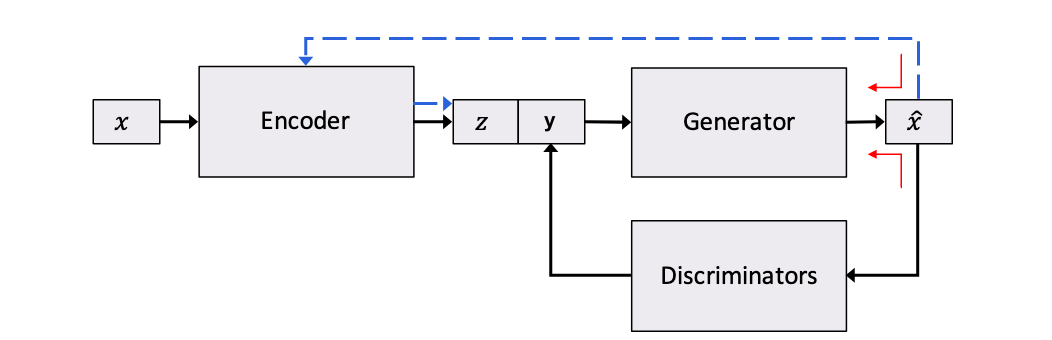
\includegraphics[scale=0.4]{control_gen_overview_edited}
	\caption{Abbildung der Idee von ControlGen}
	\label{fig:control_gen_overview}
\end{figure}
\noindent
Für jedes Merkmal (Label) in $y$ gibt es einen individuellen Diskriminator, um zu messen, wie gut die erzeugten Daten
mit den gewünschten Attributen übereinstimmen. Ausserdem werden diese Diskriminatoren gebraucht um die semantische
Struktur der einzelnen Codes zu entschlüsseln. Dies soll wiederrum den Generator dazu antreiben, bessere Ergebnisse zu
erzeugen, sowie den Latentcode anzupassen.
\newline
\newline
Wenn es einen interpretierbaren Code $y$ gibt, welcher den Output des Generators kontrolliert, muss sichergestellt
werden, dass die verschiedenen Codes nicht voneinander abhängen und sich gegenseitig beeinflussen. Dies ist vor allem
das Problem bei Attributen, welche nicht explizit abgebildet werden möchten. Diese Unabhängigkeit wird erreicht durch
Erzwingen, dass die irrelevanten Attribute vollständig im unstrukturierten Code $z$ abgebildet werden müssen.
\newline
\newline
Durch die Aufteilung des Latentspaces in unstrukturierten Code $z$ und strukturierten Code $y$ kann die Generierung der
Daten vollständig kontrolliert werden. Wenn der Code $y$ gleich bleibt und $z$ zufällig generiert wird, können zum
Beispiel Sequenzen erzeugt werden, welche die gleichen Attribute haben (z.B. $klexikon$, $wikipedia$) jedoch vom Inhalt
komplett verschieden sind. Ausserdem ist es durch diese Aufteilung möglich, den Style Transfer zu kontrollieren. Wenn
ein Satz durch den \gls{VAE} Encoder auf den unstrukturierten Code $z$ abgebildet wird und nur der strukturierte Code
(Label) $y$ abgeändert wird, ist es möglich diese beiden Inputs dem Generator zu übergeben. Dieser generiert daraus ein
Satz, welcher das gleiche Aussagt, jedoch sein Stil (strukturiertes Attribut) geändert wurde.
\newline
\newline
Der Latentcode $(z, y)$ wird aus den Daten erlernt. Der unstrukturierte Code $z$ wird durch ein unsupervised Training
(d.h. die Daten müssen keine Labels enthalten) erlernt durch das konstante Feeback der Diskriminatoren. Wobei der
strukturierte Code $y$ gelabelte Daten (Supervised) braucht um trainiert zu werden, denn $y$ soll die semantischen
Attribute der Sequenzen so optimal wie möglich abbilden.

\subsubsection{Hyperparameter}
\label{sub:crontrol_gen_hyperparameter}
In diesem Abschnitt werden die einzelnen Hyperparameter und deren Interpretation aufgelistet. Diese können verwendet
werden, um die Architektur besser an gewisse Eigenheiten der Problemstellung anzupassen, dies wird Hyperparameter
Optimierung genannt.
\begin{table}[ht]
	\centering
	\begin{tabular}{| l | l |}
	\hline
	\textbf{Hyperparameter} & \textbf{Interpretation}                                     \\ \hline
	max epochs              & Maximale Anzahl an Epochen die das Modell trainiert wird    \\ \hline
	batch size              & Anzahl an Batches in einer Epoche                           \\ \hline
	pretrain epochs         & Wieviele Epochen die Reconstruction und die Diskriminatoren \\
	                        & trainiert werden soll                                       \\ \hline
	learning rate           & Wie stark die Funktion sich in die Richtung des             \\ 
	                        & Minimums bewegen soll                                       \\ \hline
    max length sentences    & Maximale Länge der einzelnen Sätze                          \\ \hline  
	dropout rate            & Wie gross der Dropout des Modelles ist                      \\ \hline
	number of layers        & Wie viele Schichten der Encoder und Decoder haben           \\ \hline
	loss rec weight         & Wie stark der Reconstruction Loss gewichtet wird            \\ \hline
	trim padding            & Ob die generierten und echten Sätze von der selben          \\
	                        & Länge sein sollen                                           \\ \hline
	word embedding          & Welches Word Embedding verwendet werden soll, ob es gelernt \\
	                        & wird als Embedding Layer oder Fasttext verwendet wird       \\ \hline
	dimension embedding     & Dimension des verwendeten Embedding Layers                  \\ \hline
	dimension y             & Dimension des strukturierten Latentcode $y$                 \\ \hline
	dimension z             & Dimension des unstrukturierten Latentspace $z$              \\ \hline
	$\rho$ (rho)            & Wie stark der Generator Loss gewichtet werden soll          \\ \hline        
	$\gamma$ (gamma)        & Wie grosser Anteil der Softmax Funktion im Decoder ist      \\ \hline
	filter sizes            & Wie gross die einzelnen Filterkernels der Layers sind       \\ \hline
	number of filters       & Anzahl der Filters pro Convolution Schicht                  \\ \hline             
	\end{tabular}
	\caption{Hyperparameter des ControlGen Modell}
	\label{tab:hyperparameter_control_gen}
\end{table}

\subsection{CrossAlign}
\label{sub:cross_align}
In der wissenschaftlichen Arbeit (\cite{shen2017style}) in welcher die CrossAlign Architektur vorgestellt wird, ist der
Fokus auf dem Übertragen von Stilen aufgrund von nicht-parallelen Daten. Darin wird das Trennen von Stil und Inhalt als
grösste Herausforderung gesehen, welches mittels dem neu entwickelten Modell gelöst werden soll.
\newline
\newline
Um ein Attribut des Satzes, wie z.B. den Stil, unabhängig vom Inhalt zu kontrollieren, muss es möglich sein den Stil von
anderen Attributen vollständig zu lösen. Das Problem ist jedoch, dass viele verschiedene Attribute miteinander
interagieren, vor allem in Sprachen, wo die Grammatik eine wichtige Rolle spielt.
\newline
\newline
Das Ziel dieses Modells ist es, die Verteilungsäquivalenz von Inhalten zu nutzen, um einen Satz in einem Stil auf einen
stilunabhängigen Inhaltsvektor abzubilden und diesen dann in einen Satz mit dem gleichen Inhalt, aber einem anderen Stil
zu dekodieren. Diese Verteilungsäquivalenz nimmt nur an, dass die Daten in den beiden unabhängigen Domänen die selbe
Verteilung des Inhaltes haben.
\newline
\newline
Das Netzwerk besteht aus einem Encoder, welcher einen Satz und seinen ursprünglichen Stil als Eingabe nimmt und diesen
auf eine stilunabhängige Inhaltsrepräsentation abbildet. Sowie stilabhängige Generatoren, welche die
Inhaltsrepräsentation ohne Stil zu einer Repräsentation mit Stil umwandeln. Für diesen Prozess werden keine typischen
\gls{VAE} verwendet, da es zwingend notwendig ist, die Darstellung der latenten Inhalte reichhaltig und störungsfrei
abzubilden.
\begin{figure}[H]
	\centering
	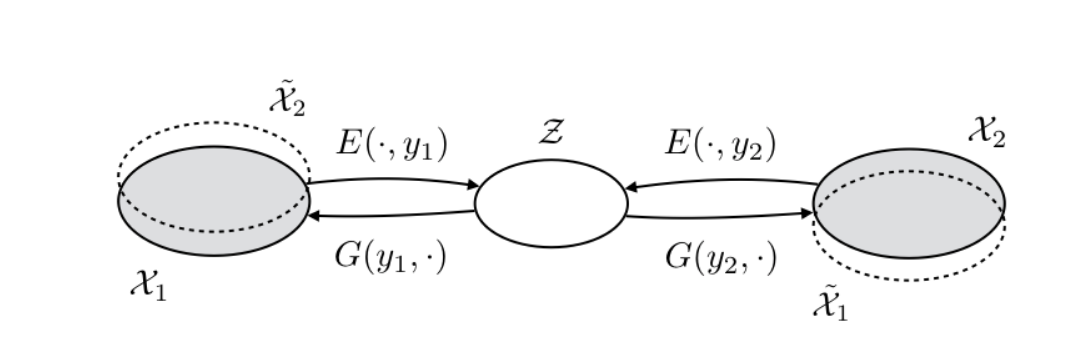
\includegraphics[scale=0.35]{cross_align_overview}
	\caption{Abbildung der Idee von CrossAlign}
	\label{fig:cross_align_overview}
\end{figure}
\noindent
In Abbildung \fullref{fig:cross_align_overview} ist die allgemeine Idee von der CrossAlign Arbeit ersichtlich. $X_1$ und
$X_2$ sind zwei Datensätze mit unterschiedlichen Stilen $y_1$ und $y_2$, z.B. $y_1 = klexikon$ und $y_2 = wikipedia$.
$Z$ ist der gemeinsame Latentspace. Der Encoder $E$ projiziert eine Sequenz auf den gemeinsamen Latenspace $Z$ und
Generator $G$ generiert den Satz zurück wenn dieser mit dem ursprünglichen Stil kombiniert wird. Wenn eine
Inhaltsrepräsentation mit einem anderen Stil dem Generator übergeben wird, transferiert dieser die Sequenz in einen
anderen Stil $\tilde{X_1}$. 
\newline
\newline
Im Datensatz $X$ gibt es verschiedene Sequenzen $X = \{x^{(1)},..., x^{(n)} \}$ welche von der gleichen bedingten Verteilung
$p(x|y,z)$ stammen. Diese Verteilung hängt von der Latent Style Variable $y$ und der Latent Content Variable $z$ ab,
wobei beide Variablen unbekannt sind. Wichtig ist, dass $X$, der aus verschiedenen Stilen generiert
wird, unterschiedlich genug sein sollte, da sonst die Transferaufgabe zwischen den Stilen nicht gut definiert ist. Dies
erscheint zwar trivial, kann aber auch bei vereinfachten Datenverteilungen nicht immer gelten.

\subsubsection{Hyperparameter}
\label{sub:crontrol_gen_hyperparameter}
In diesem Abschnitt werden die einzelnen Hyperparameter und deren Interpretation aufgelistet. Diese können verwendet
werden, um die Architektur besser an gewisse Eigenheiten der Problemstellung anzupassen, dies wird Hyperparameter
Optimierung genannt.
\begin{table}[ht]
	\centering
	\begin{tabular}{| l | l |}
	\hline
	\textbf{Hyperparameter} & \textbf{Interpretation}                                     \\ \hline
	max epochs              & Maximale Anzahl an Epochen die das Modell trainiert wird    \\ \hline
	batch size              & Anzahl an Batch in einer Epoche                             \\ \hline
	learning rate           & Wie stark die Funktion sich in die Richtung des             \\ 
	                        & Minimums bewegen soll                                       \\ \hline
    max length sentences    & Maximale Länge der einzelnen Sätze                          \\ \hline  
	dropout rate            & Wie gross der Dropout des Modelles ist                      \\ \hline
	number of layers        & Wie viele Schichten der Encoder und Decoder haben           \\ \hline
	loss rec weight         & Wie stark der Reconstruction Loss gewichtet wird            \\ \hline
	trim padding            & Ob die generierten und echten Sätze von der selben          \\
	                        & Länge sein sollen                                           \\ \hline
	word embedding          & Welches Word Embedding verwendet werden soll, ob es gelernt \\
	                        & wird als Embedding Layer oder Fasttext verwendet wird       \\ \hline
	dimension embedding     & Dimension des verwendeten Embedding Layers                  \\ \hline
	dimension y             & Dimension des strukturierten Latentcode $y$                 \\ \hline
	dimension z             & Dimension des unstrukturierten Latentspace $z$              \\ \hline
	$\rho$ (rho)            & Wie stark der Generator Loss gewichtet werden soll          \\ \hline        
	$\gamma$ (gamma)        & Wie grosser Anteil der Softmax Funktion im Decoder ist      \\ \hline
	filter sizes            & Wie gross die einzelnen Filterkernels der Layers sind       \\ \hline
	number of filters       & Anzahl der Filters pro Convolution Schicht                  \\ \hline             
	\end{tabular}
	\caption{Hyperparameter des CrossAlign Modell}
	\label{tab:hyperparameter_cross_align}
\end{table}

\section{Training der Modelle}
\label{sec:training_der_modelle}

In diesem Kapitel, \fullref{sec:training_der_modelle}, wird der Aufbau des Trainings der Modelle beschrieben. Es geht
darum die Modelle aus \fullref{sub:modelle} auf den in \fullref{sec:aufbau_datensatz} aufgebauten Datensätzen zu
trainieren. Die Resultate und Weiterführungen der einzelnen Trainings werden in \fullref{sec:resultate} vorgestellt.

\subsection{Verwendete Codebasis}
\label{sub:verwendete_codebasis}

Für das Training der Modelle wurde eine bestehende Codebasis verwendet. Dies aufgrund fehlender Ressourcen, sowie
Erfahrung, eine neue Implementation für die Modelle zu entwickeln. Als Codebasis dient das Github-Repository der
Forschungsgruppe (\cite{Li2019DomainAT}) verwendet. Das Original Repository findet sich auf GitHub unter
https://github.com/cookielee77/DAST (\cite{cookielee77_dast}).
\newline
\newline
Die Codebasis wurde zwecksmässig angepasst. Dabei wurden nicht verwendete Codeteile entfernt. Weiter wurden die Basis
mit für das Projekt nötige Implementation angepasst. Die ursprüngliche Base beinhaltet dabei die Implementation für das
Modell aus \fullref{sub:control_gen} und \fullref{sub:cross_align}. Die Implementationen sind mit Python (\cite{python})
und Tensorflow (\cite{tensorflow}) umgesetzt. 
\newline
\newline
Dabei wurde für die Umsetzung des Wirtschaftsprojekt folgende Erweiterungen für die Codebasis implementiert.

\begin{itemize}
  \setlength\itemsep{0em}
  \item Erweiterung des Projektes mit einem Prototyp um die Modelle manuell zu testen
  \item Erweiterung der Trainings und Evaluations Metriken mit \gls{METEOR} und \gls{WER}
  \item Erweiterung der Funktionalität vom Embedding Layer der einzelnen Modellen, um Fasttext zu verwenden
  \item Kontrolle über die Gewichtung des Reconstruction Loss
  \item Kontrolle über die Anzahl der minimalen Vorkommnisse der Wörter im Vokabular
  \item Umfangreiche Unittests der einzelnen Modelle
  \item Logging der Hyperparameter
  \item Visualisierung der einzelnen Modelle auf dem Tensorboard
\end{itemize}
\noindent

\subsection{Verwendete Trainingsumgebung}
\label{sub:verwendete_trainingsumgebung}
Um ein effizientes Training der Modelle zu ermöglichen, sind entsprechend Rechenressourcen notwending. Privat standen
keine aussreichende Rechener zur verfügung um das Training durchzuführen. Um eine möglichst flexible Gestaltung der
Zeiten für das Training zu ermöglichen, wurde entschieden auf http://vast.ai (nachfolgend vast.ai) zurückzugreifen. Bei
vast.ai können Grafikkarten für Berechnungen angemietet werden. Diese werden über ein Docker Container bereitgestellt.
Der benötigte Code, sowie der Datensatz, wurden in den Container eingespielt. Anschliessend konnte für die Mietdauer die
Grafikkarte verwendet werden. Dabei wurden Grafikkarten vom Typ Nvidia GeForce (\cite{wikipedia_2019_geforce}) verwendet, hauptsächlich die Modelle
Titan X und 1080Ti.

\subsection{Trainingsplanung}
\label{sub:ablauf_und_resultate}
Damit die Trainings der Modelle einem geregeltem Ablauf folgen, wird eine Trainingsplanung durchgeführt. Wie in
\ref{sec:resultate} eingesehen werden kann, geht es darum, die Hyperparameter der beiden Modelle anzupassen. Damit
sollen die Modelle den \gls{NST} auf den beiden Datensatz möglichst genau durchführen. Weiter werden zu Beginn, wie in
\ref{sub:standard_hyperparameter} beschrieben, die Modelle auf beiden Datensätzen, \flqq Ausgeglichen\frqq \ und \flqq Gekürzt\frqq,
trainiert. Auch sollen zuerst die standard Hyperparameter der Autoren der beiden Ansätze verwendet werden. So können die
Modelle ein erstes Mal auf ihre Leistung geprüft werden. Anschliessend können aufgrund der Ergebnisse der ersten
Trainings die Hyperparameter angepasst werden. Um die Resultate gegeneinader vergleichbar zu halten, werden alle
Trainings mit $ 200 $ \gls{Epoche} trainiert.


\chapter{Methode}
\label{ch:Methode}
Im Kapitel \fullref{ch:Methode} werden die verwendeten Methoden vorgestellt. Dabei geht es um die Definition der
Problemstellung, sowie der Projektabgrenzung.

\section{Vorgehensmodell}
\label{sec:Vorgehensmodell}
Dieses Projekt wurde mittels einem explorativen Vorgehensmodell umgesetzt, da sich dieses Modell optimal für ein
Innovation- / Forschungsprojekt anwenden lässt. Ausserdem wird in diesem Modell die kreative Problemlösung mittels
mehreren Lernzyklen gefördert, was in einem Innovationsprojekt ein Muss ist. Dieses Modell wird in Grafik
\ref{fig:Meilensteinplanung} dargestellt.
\newline
\newline
In einer ersten Phase, der Initialisierungsphase, wird das Projekt genauer untersucht sowie allfällige Fragen und
Unwissenheiten geklärt. Nach der Initialisierungsphase sollte klar sein, was genau mit der Arbeit erreicht werden soll
und welches die grössten Schwierigkeiten sind. 
\newline
\newline
Anschliessend gibt es eine divergierende Ideenfindungsphase, in der der aktuelle Stand der Technik untersucht wird und
verschiedene Ansätze erforscht werden. In dieser Phase sollten auch verschiedene Experimente durchgeführt werden, um die
Machbarkeit besser zu beurteilen. Nach dieser Phase sollte klar sein, welche Ansätze in Frage kommen, um das Projekt
umzusetzen.
\newline
\newline
Nach der divergierenden Phase kommt die konvergierende Ideenfindungsphase, in der das Ziel ist, aus den vorher
erforschten Methoden wenige auszuwählen und genauer zu untersuchen. So kann die Anwendbarkeit auf das Projekt beurteilt
werden. Nach dieser Phase sollten nur noch etwa 1-2 Ideen bestehen, welche die Problemstellung optimal angehen und einen
vielversprechenden Ansatz zur Lösung dieser bieten.
\newline
\newline
Die letzte Phase in diesem Vorgehensmodell ist die Umsetzungsphase, diese beinhaltet die komplette Umsetzung der Idee
mittels den erforschten Ideen aus den vorherigen Phasen. Dabei geht es vor allem darum die Problemstellung so weit wie
möglich zu lösen und auch Vorschläge für die Umsetzung anderer Ideen in der gleichen Domäne zu geben. Nach der
Umsetzungsphase sollte das Projekt abgeschlossen sein und ein Prototyp sowie eine klare Forschung zum jeweiligen
Themengebiet ersichtlich sein.
\begin{figure}[H]
	\centering
	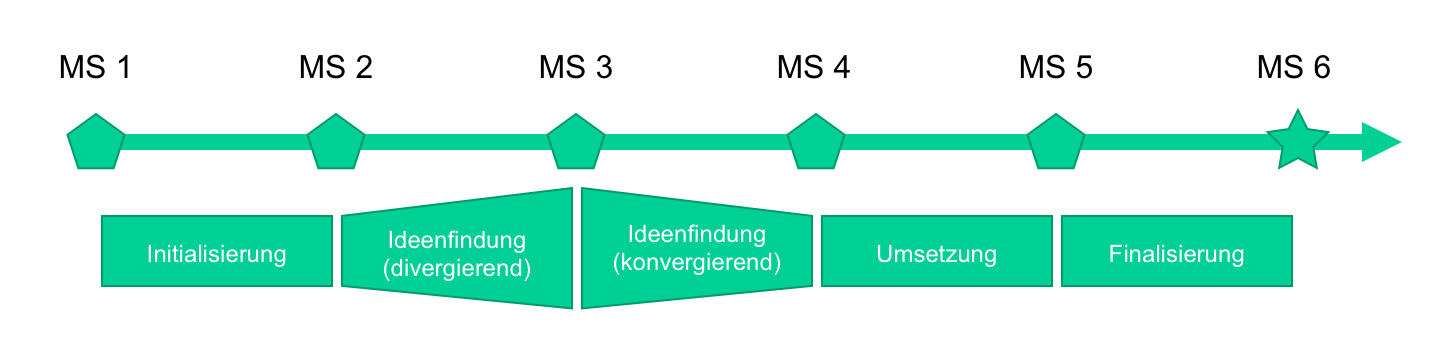
\includegraphics[scale=0.3]{Meilensteinplanung}
	\caption{Meilensteinplanung}
	\label{fig:Meilensteinplanung}
\end{figure}
\noindent

\subsection{Meilensteinplanung}
\label{sec:Meilensteinplanung}
Die Meilensteinplanung ist im explorativen Vorgehensmodell naheliegend, nach jeder abgeschlossenen Phase gibt es einen
neuen Meilenstein, sowie beim Start und bei der Abgabe. Demnach gibt es insgesamt $ 6 $ Meilensteine, die erreicht
werden sollen. Die Termine der Meilensteine ergeben sich aus der Zeitplanung des Herbstsemesters an der HSLU und den
Rahmenbedingungen des Moduls \flqq Wirtschaftsprojekt\frqq. Die detaillierten Berichte zu den einzelnen Meilensteinen
können im Anhang eingesehen werden unter \fullref{app:meilensteinberichte}.
\begin{itemize}
	\setlength\itemsep{0em}
	\item \textbf{M1: 26. September 2019}, Start des Projektes
	\item \textbf{M2: 10. Oktober 2019}, Ende Initialisierungsphase
	\item \textbf{M3: 21. Oktober 2019}, Ende Ideenfindungsphase divergierend
	\item \textbf{M4: 11. November 2019}, Ende Ideenfindungsphase konvergierend
	\item \textbf{M5: 9. Dezember 2019}, Ende Umsetzungsphase
	\item \textbf{M6: 20. Dezember 2019}, Ende Finalisierung und Abgabe Projekt
\end{itemize}

\section{Problemstellung}
\label{sec:Problemstellung}
Die Aufgabenstellung wird bereits in Kapitel \fullref{sec:Aufgabenstellung-Zielsetzung} ausgeführt. Für die
Problemstellung soll anhand der Bausteine des Zeugnismanagers und ansprechenderen Sätze das Problem aufgezeigt werden. 
\newline
\newline
Im Zeugnismanager können Arbeits-, sowie Zwischenzeugnisse, für Mitarbeitende erstellt werden. Der Baukasten umfasst
dabei die Sprachen Deutsch, Französisch, Italienisch und Englisch. Weiter sind die Bausteine für Mitarbeiter beider
Geschlechter vorhanden. Arbeits- und Zwischenzeugnis unterscheidet sich anhand der Zeitform, wobei das Arbeitszeugnis in
Präteritum, das Zwischenzeugnis in Präsens verfasst wird.
\newline
\newline
Der Benutzer des Zeugnismanagers kann mithilfe von verschiedenen Bewertungskategorien, die Leistungen des zu bewertenden
Mitarbeiters beurteilen. Für jede Kategorie kann eine Bewertung zwischen $A$ und $D$ abgegeben werden, wobei A den oberen
Teil der Skala markiert. Für die entsprechenden Bewertung stehen anschliessend verschiedene Textbausteine zur Auswahl.

\begin{figure}[H]
	\centering
	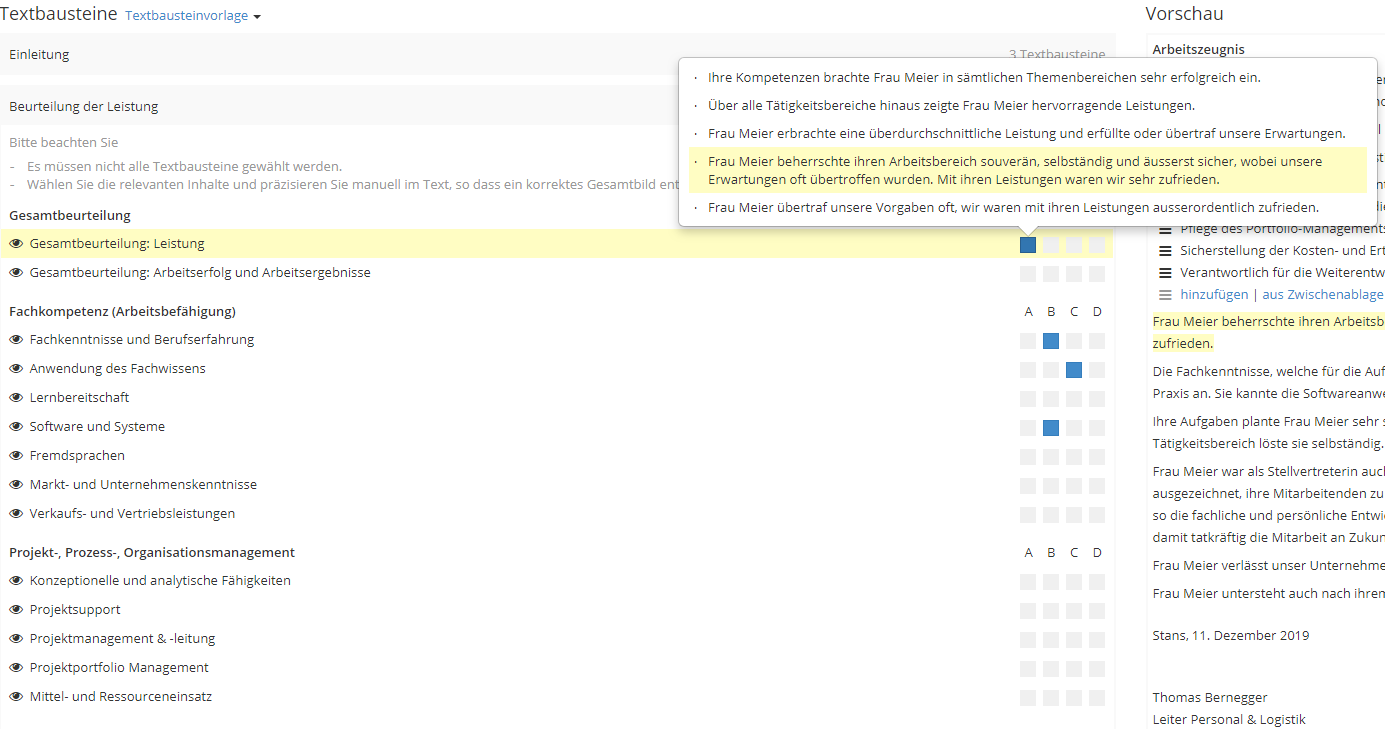
\includegraphics[scale=0.275]{zeugnismanager_narrow.png}
	\caption{Screenshot Zeugnismanager}
	\label{fig:screenshot_zeugnismanager}
\end{figure}
\noindent
\newline
Dabei sind die unten aufgeführten Sätze Beispiele für eine Bewertungskategorie mit der Bewertung A.
\begin{enumerate}
	\setlength\itemsep{0em}
	\item \textit{Herr Foo schaffte die Voraussetzungen für ein leistungsförderndes Arbeitsklima und unterstützte aktiv den konstruktiven Austausch im Team.}
	\item \textit{Herr Foo schaffte die Voraussetzungen für ein konstruktives und leistungsförderndes Arbeitsklima.}
	\item \textit{Herr Foo schaffte die nötigen Voraussetzungen für ein leistungsförderndes Arbeitsklima und eine konstruktive Zusammenarbeit.}
\end{enumerate}

Für tiefere Bewertungen stehen oft weniger Textbausteine zur Verfügung.
\begin{enumerate}
	\setlength\itemsep{0em}
	\item \textit{Die Zusammenarbeit im Team förderte Herr Foo nicht mit dem nötigen Engagement.}
\end{enumerate}
\noindent
Ein beispielhaftes Arbeitszeugnis, welches mit dem Zeugnismanager erstellt wurde, ist im Anhang zu finden
\fullref{ch:beispiel_arbeitszeugnis}. Die meisten Kunden des Auftraggebers editieren nach dem Erstellen des Zeugnisses
den Text, um das holprige Lesen zu verhindern. Die Unternehmen können die Textbausteine frei editieren, um bereits beim
Erstellen der Zeugnisse den Lesefluss zu fördern. Ein qualitativ hochwertiges Arbeitszeugnis, kann aufgrund des
Datenschutzes nicht angehängt werden. Jedoch soll anhand einiger Beispielsätze gezeigt werden, welche Qualität
angestrebt werden soll.
\begin{enumerate}
	\setlength\itemsep{0em}
	\item \textit{Bei der Ausübung seiner Aufgaben zeichnet er sich aus durch eine äusserst selbständige und effiziente Arbeitsweise, Beharrlichkeit sowie hohes Qualitäts- und Kostenbewusstsein.}
	\item \textit{Herr Foo ist Neuerungen gegenüber \textbf{offen, erkennt} Innovationsmöglichkeiten und bringt konkret umsetzbare Ideen ein.}
	\item \textit{Er pflegt eine offene Kommunikationskultur und informiert \textbf{zeit- und stufengerecht.}}
\end{enumerate}
\noindent
Dabei ist auf die Verschachtlung und Referenzen in den einzeln Sätzen zu achten. In den Textbausteinen des
Zeugnismanagers beschränkt sich die Verschachtlung auf Aufzählungen.

\section{Lösungsansatz}
\label{sec:Lösungsansatz}
Für die Lösung der Aufgabenstellung könnten verschiedene Ansätze verwendet werden, siehe
\fullref{sec:empfehlung_zeugnismanager}. Die Arbeitszeugnis des Zeugnismanagers zeugen bereits von guter Qualität. Sie
vermögen es jedoch nicht mit der Qualität von individuell geschriebener Zeugnisse mitzuhalten.
\newline
\newline
Da der Zeugnismanager wie erwähnt bereits ein auf dem Markt konkurrenzfähiges Produkt ist, käme die Umgestaltung des
Manager oder der Textbausteine einer Weiterentwicklung gleich. Dies ist nach Absprache mit dem Auftraggeber und des
Betreuer nicht das Ziel dieser Arbeit. Es soll daher ein neuer Ansatz gesucht werden, welcher ein Alleinstellungsmerkmal
für die Marktlösung des Auftraggebers sein kann. Weiter soll der Lösungsansatz im Bereich des maschinellen Lernen
angesiedelt sein, siehe \fullref{ch:aufgabenstellung}.
\newline
\newline
Für das Errechnen der Modelle ist ein grosser Datensatz nötig. Die Daten sollten dabei aus dem entsprechenden
Anwendungsgebiet stammen. Für die Umsetzung solcher Lösungen sind im Falle für Arbeitszeugnisse bedauerlicherweise nicht
genügend Daten vorhanden. Für die Arbeit soll daher ein Datensatz aufgebaut werden, welches das Problem abbildet. Anhand
des Datensatzes sollen Modelle für die Problemlösung evaluiert werden. Die Modelle sollen dabei den Style Transfer
vornehmen. Daher wurde entschieden einen Datensatz aufzubauen, welcher das Problem abbildet. Wie in
\fullref{sec:Problemdefinition} beschrieben geht es darum den Stil eines Satzes zu ändern. Es wird nun nach Daten
gesucht, die aus dem selben Themengebiete stammen und verschiedene Schreibstile aufweisen. Dabei werden die Stillabels $
holprig $ und $ flüssig $ durch Stillabels des verwendeten Datensatzes ersetzt. Der Datensatz sowie die neuen Stillabel
werden in \fullref{sec:verwendeter_datensatz} beschrieben.

\section{Evaluierung}
\label{sec:method_eval}
Die Evaluierung der Arbeit ist einer der wichtigsten Punkte des Projektes, denn dadurch soll festgestellt werden ob die
verfolgten Ansätze zum Lösen des Problemstellung vielversprechend sind und diese weiter verfolgt werden sollen.
\newline
\newline
Eine weiter Methode zur Überprüfung, ist die Messung der Verteilung des Datensatzes vor und nach dem Transfer. Damit
soll überprüft werden ob sich die Verteilung nach dem Transfer deutlich von der Vorherigen unterscheidet. Die neue
Verteilung sollte aufzeigen, dass die Sätze vor allem länger werden. Jedoch kann die Komplexität der
einzelnen Sätze nur schlecht statistisch gemessen werden und muss daher manuell gemacht werden.
\newline
\newline
Weiter sollen die Sätze manuell überprüft werden. Dabei werden diese vor und nach dem Transfer genauer betrachtet. So
kann abgeschätzt werden ob der Satz korrekt in die neue Domäne gebracht wurde. Ausserdem soll auf die Grammatik der
generierten Sätze geachtet werden um zu beurteilen ob diese korrekt erlernt wurde.

\section{Testing}
\label{sec:methode_test}
Um die Funktionsfähigkeit der Modelle sicherzustellen müssen diese automatisiert und nachvollziehbar getestet werden
können. Um diese Art von Testing zu gewährleisten, werden Unit Tests (\cite{unit_test}) verwendet. Diese können automatisiert ausgeführt
werden und testen immer den gleichen Ablauf mit vordefinierten Parametern. Unit Tests sollten immer nur einen Fall
testen, was in diesem Projekt auch so umgesetzt wurde.
\newline
\newline
Jedes verwendete Modell wird separat mit den gleichen Testfällen auf Richtigkeit überprüft. Die Modelle werden auf vier
solcher Testcases überprüft:
\begin{enumerate}
	\setlength\itemsep{0em}
	\item Testen ob die trainierbaren Variablen sich nach einem Trainingsschritt verändern
	\item Testen ob der Loss nach einem Trainingsschritt nicht Null ist
	\item Testen ob der Diskriminator separat von dem Generator trainiert werden kann
	\item Testen ob das Modell einen Output liefert
\end{enumerate}
\noindent
Durch diese vier Testfälle kann sichergestellt werden, dass das Modell trainiert werden kann und keinen Fehler in
der Architektur vorhanden sind und die einzelnen Schichten korrekt miteinander verbunden sind. Ausserdem kann durch
Testcase $3$ vergewissert werden, dass bei einem \gls{GAN} die beiden Komponenten separat voneinader trainiert werden
können. Jeder einzelne dieser Testfälle muss korrekt durchlaufen nach einer Änderung des Modells und am Schluss des
Projektes.

\section{Aufbau Projekt}
\label{sec:aufbau_projekt}
Das Projekt wurde in vier verschiedene Git Repositories unterteilt, um die einzelnen Schritte der Umsetzung sinnvoll zu
trennen. Diese werden im folgenden Abschnitt genauer beschrieben.

\subsection{wipro-doc}
\label{sub:wipro-doc}
In diesem Repository befindet sich die ganze Dokumentation des Projektes, sowie das Verzeichnis welches für die
Recherche der Arbeit gebraucht wird. Dieses Repository wird immer wieder bearbeitet und beinhaltet schlussendlich auch
die finale Dokumentation, welche abgegeben wird.
\newline
Link zum Git Repository: \hyperlink{https://gitlab.enterpriselab.ch/Pwn3rs/wipro-doc}{wipro-doc}
\newline
\dirtree{%
.1 wipro-doc.
.2 assets \ldots{} (assets for the project).
.2 documentation \ldots{} (latex file for final documentation).
.2 research \ldots{} (markdown file for research).
.2 study-doc \ldots{} (origin of study-doc).
}

\subsection{wipro-data}
\label{sub:wipro-data}
Wird verwendet, um die ganzen Daten, welche im Projekt genutzt werden, an einem zentralen Ort zu speichern. Darin sind
mehrere Datensätze vorhanden, welche im Repository aufbereitet und statistisch analysiert werden. Dieses Git Projekt ist
ein Git LFS Repository, da es sich um grosse Files handelt.
\newline
Link zum Git Repository: \hyperlink{https://gitlab.enterpriselab.ch/Pwn3rs/wipro-data}{wipro-data}
\newline
\dirtree{%
.1 wipro-data.
.2 utils \ldots{} (util classes for cleaning, processing the data).
.2 cleaned \ldots{} (cleaned data).
.2 crawled \ldots{} (crawled data).
.2 notebooks \ldots{} (jupyter notebooks for prepare, process and analyze data).
.2 processed \ldots{} (processed data).
.2 statistics \ldots{} (statistic data).
}

\subsection{wipro-source}
\label{sub:wipro-source}
Dieses Projekt beinhaltet die ganze Codebasis dieser Projektarbeit. Es ist dafür da, um verschiedene Modelle zu testen
und zu evaluieren. Darin befinden sich auch Datensätze von \textit{wipro-data}, um die entsprechenden Modelle damit zu
trainieren. In diesem Repository befindet sich ausserdem der Prototyp der Arbeit.
\newline
Link zum Git Repository: \hyperlink{https://gitlab.enterpriselab.ch/Pwn3rs/wipro-source}{wipro-source}
\newline
\dirtree{%
.1 wipro-source.
.2 data \ldots{} (data to train the models).
.2 dataloader \ldots{} (loads data for the models to process).
.2 network \ldots{} (architecture of the models).
.2 notebooks \ldots{} (jupyter notebooks to analyze models).
.2 save-model \ldots{} (saved models).
.2 test \ldots{} (unit tests for the networks).
.2 prototype.py \ldots{} (prototype of the project).
}

\subsection{wipro-logs}
\label{sub:wipro-logs}
In diesem Git Projekt befinden sich Log Files, Tensorboard Daten und Testsätze aller trainierten
Modelle. Dies wird zum Hyperparametertuning sowie zur Evaluierung gebraucht. In diesem Repository kann Tensorboard
gestartet werden und somit die entsprechenden Graphen eingesehen werden. Zu jedem trainierten Modell gibt es im
\textit{logs} Ordner ein entsprechende Verzeichnis mit den Daten.
\newline
Link zum Git Repository: \hyperlink{https://gitlab.enterpriselab.ch/Pwn3rs/wipro-logs}{wipro-logs}
\newline
\dirtree{%
.1 wipro-logs.
.2 log-archive \ldots{} (archive of the first models trained logs).
.2 logs \ldots{} (logs of the trained models).
.3 Classifier \ldots{} (logs of the classifiers).
.3 ControlGen \ldots{} (logs of the ControlGen models).
.3 CrossAlign \ldots{} (logs of the CrossAlign models).
.2 Tensorboard.ipynb \ldots{} (jupyter notebook to start tensorboard).
}


\chapter{Realisierung}
\label{ch:Realisierung}
% TODO Beschreibung der Umsetzung der definierten Ziele, einschliesslich der aufgetretenen Schwierigkeiten und Einschränkungen
In diesem Kapitel wird die ganze Realisierung des Projektes beschrieben, einschliesslich der aufgetretenen
Schwierigkeiten und Einschränkungen. Dabei geht es darum, die Umsetzung der definierten Ziele aufzuzeigen.

\section{Aufbau Datensatz}
\label{sec:aufbau_datensatz}
Wie in Kaptiel \fullref{sec:abschliessende_problemdefinition} beschrieben, wird ein Datensatz mit Texten aufgebaut,
welchem dem Label $ erwachsen $, sowie dem Label $ kindlich $ zugeteilt werden können. Die Quellen der Texte sind Online
Lexikas. Wikipedia dient dabei als Quelle für Sätze des Labels $ erwachsen $, analog dient das Klexikon als Quelle für
Sätze des Labels $ kindlich $. Für das Zusammentragen der Texte wurde ein Crawler realisiert, welcher die Artikel aus
dem Klexikon und Wikipedia zusammenträgt.

\subsection{Reinigung des Datensatz}
\label{sub:reinigung_des_datensatz}
Die Artikel wurden entsprechend gereinigt und die einzelnen Sätze aus den Artikeln extrahiert. Dabei wurde auf das
Framework Natural Language Toolkit (NLTK) zurückgegriffen. Die Pipeline für die Reinigung und der Extrahierung wurde
dabei wie folgt aufgebaut.
\newline
\begin{enumerate}
	\setlength\itemsep{0em}
	\item Reinigung der Strings durch ersetzen von Buchstaben mit Akzent zeichen wie z.B. è, à, â, ê.
	\item Einheitliche Verwendung von Anführszeichen.
	\item Einfügen von Leerschläge bei Kommas (,), Gedankenstichen (-), Schrägstrichen (/), Doppelpunkt (:), Strichpunkt
	(;) sowie an Satzenden.
	\item Tokenizierung der Arikel zu Sätzen mithilfe von NLTK. Dabei wurden nur Sätze erlaubt, welche gewisse Charaktere
	enthalten.
	\item Anpassung der Grossschreibung der Satzanfänge mithilfe von TreeTagger. Dabei wurde die Grossschreibung nur beibehalten, falls das Wort
    ein Nomen oder Eigennamen ist.
\end{enumerate}
\noindent
Weiter wurden Daten für die statistische Analyse der Datenquelle sowie der Sätze mitaufgezeichned. Dies, um in einem
nächsten Schritt, den Datensatz weiter zu bereiningen. Für die Datenquellen wurden folgende Daten aufgezeichnet.
\begin{enumerate}
    \setlength\itemsep{0em}
    \item Anzahl an Artikel aus der Datenquelle
    \item Anzahl Sätze aus der Datenquelle
    \item Anzahl Wörter aus der Datenquelle
\end{enumerate}
\noindent
Für die Analyse der einzelnen Sätze wurde während der Reinigung der Sätze folgendes mitabgespeichert.
\begin{enumerate}
    \setlength\itemsep{0em}
    \item Datenquelle des Satzes
    \item Artikel des Satzes
    \item Anzahl Wörter im Satz
\end{enumerate}
\noindent
So entstand aus den Artikeln der einzelnen Datenquelle ein gemeinsamer Datensatz, abgespeichert als CSV, welcher
folgende Struktur aufweist.
\begin{verbatim}
source	article	length	sentence
klexikon	Aal	9	Aale sind Fische , die wie Schlangen aussehen .
klexikon	Aal	10	ihre Körper sind sehr lang , schlank und beweglich .
klexikon	Aal	13	sie haben eher kleine Flossen , die wie Bänder am Körper anliegen .
wikipedia	Reh	7	die Fluchtdistanz von Feldrehen ist hoch .
wikipedia	Reh	8	diese hohe Fluchtdistanz kompensiert die fehlende Deckung .
\end{verbatim}

\subsection{Statistische Analyse des Datensatz}
\label{sub:statistische_analyse_des_datensatz}
In einem weiteren Schritt wurde der Datensatz statistisch analysiert. Dies, um den Datensatz weiter zu reinigen und zu
normalisieren. Dabei soll zuerst die Zählung der Artikel, Sätze, sowie der Wörter aufgezeigt werden.
\begin{figure}[H]
    \minipage{0.32\textwidth}
      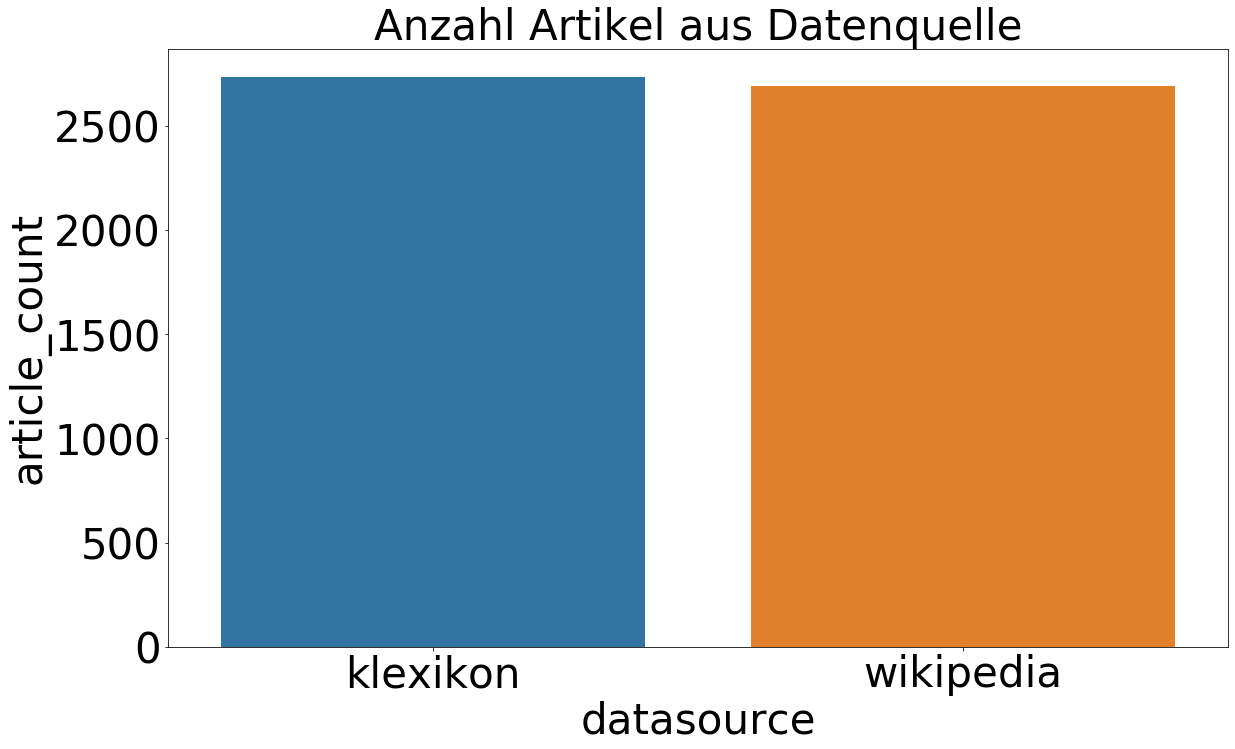
\includegraphics[width=\linewidth]{article_count_ds.png}
      \caption{Anz. Artikel im Datensatz}\label{fig:article_count_ds}
    \endminipage\hfill
    \minipage{0.32\textwidth}
      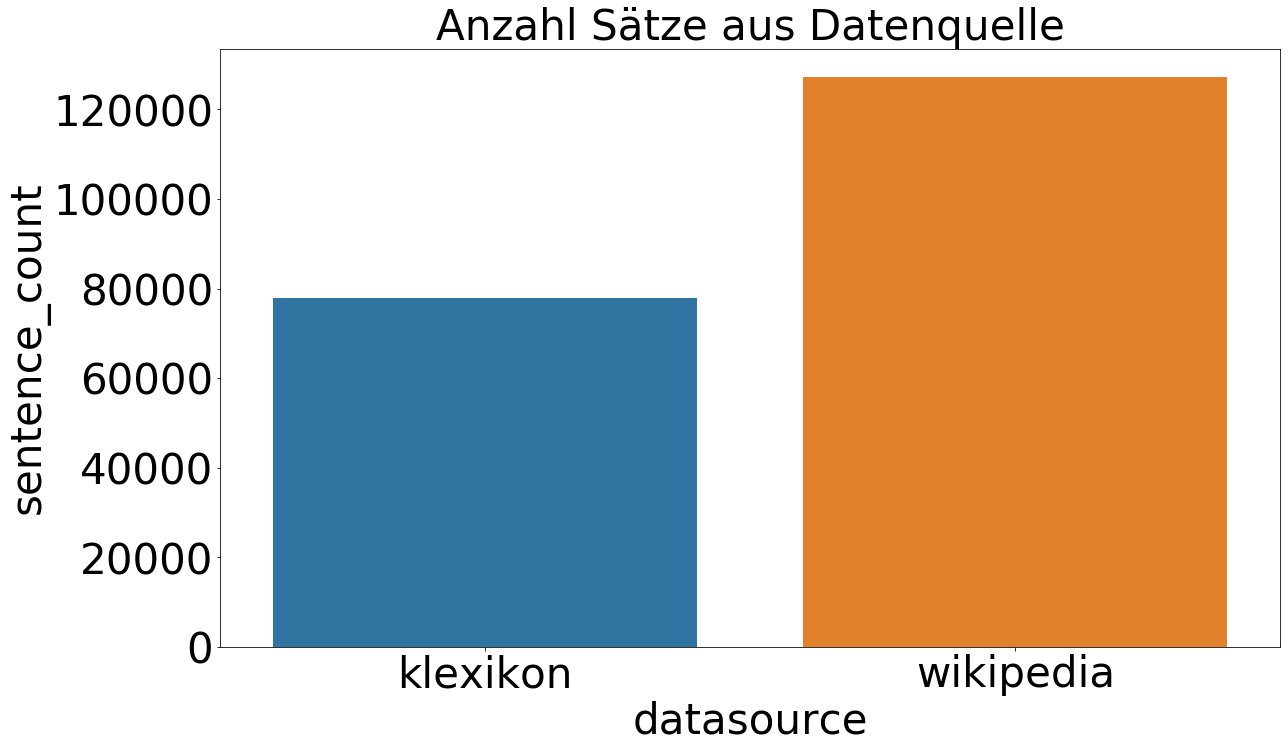
\includegraphics[width=\linewidth]{sentence_count_ds.png}
      \caption{Anz. Sätze im Datensatz}\label{fig:sentence_count_ds}
    \endminipage\hfill
    \minipage{0.32\textwidth}
      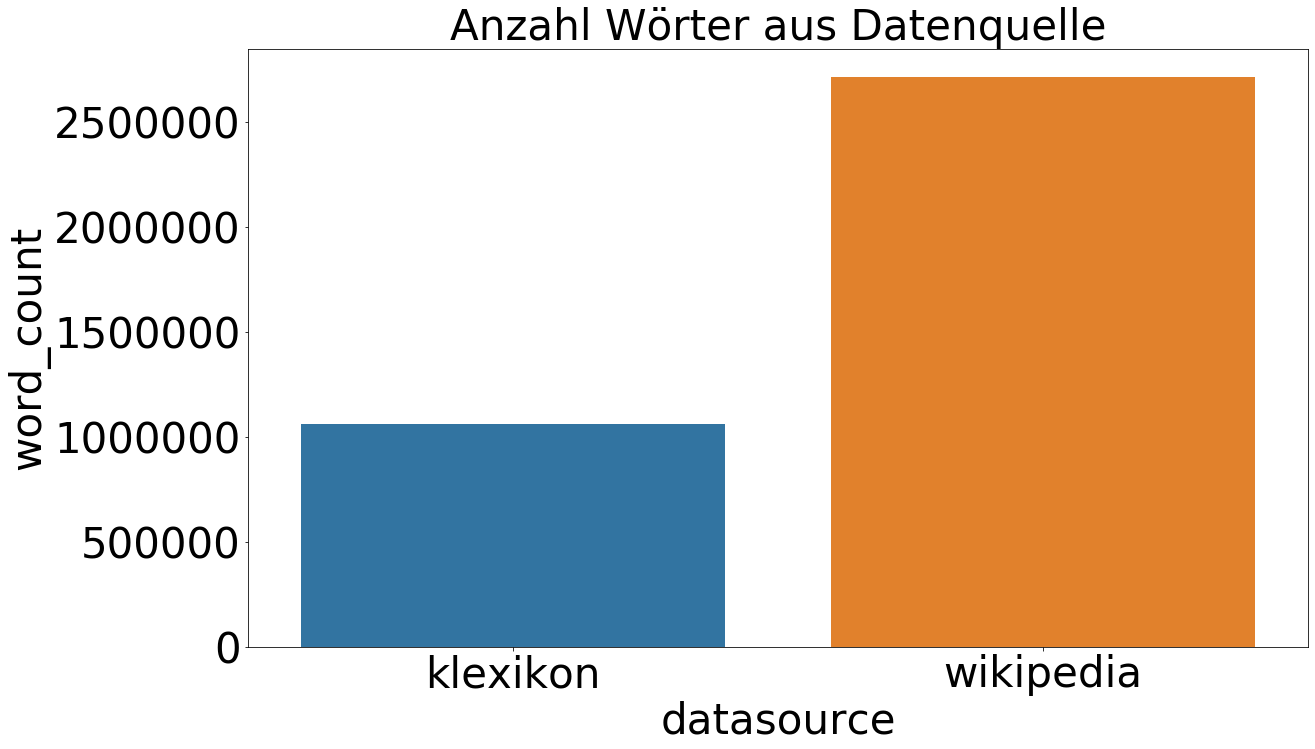
\includegraphics[width=\linewidth]{word_count_ds.png}
      \caption{Anz. Wörter im Datensatz}\label{fig:word_count_ds}
    \endminipage       
\end{figure}
\begin{table}[H]
  \centering
  \begin{tabular}{|c|c|c|c|}
      \hline
      \textbf{Datenquelle}& \textbf{Anz. Artikel}& \textbf{Anz. Sätze}& \textbf{Anz. Wörter}\\
      \hline
      \textbf{Klexikon}& 2'733 & 77'924 & 1'058'623\\
      \hline
      \textbf{Wikipedia}& 2'689 & 127'177 & 2'710'452\\
      \hline
  \end{tabular}
  \caption{Anzahl der Artikel, Sätze und Wörter aus Wikipedia und Klexikon.}
\label{tab:dataset_count_wiki_klexi_base}
\end{table}
\noindent
Wie angenommen sind die Artikel von Wikipedia umfangreicher als die vom Klexikon. Die Artikel beinhalten mehr Sätze als
aus dem Lexikon. Entsprechend auch mehr Wörter. Dies kann auch anhand der Verteilung für Sätze pro Artikel aufgezeigt
werden, siehe \ref{fig:distribution_sentence_klexi} und \ref{fig:distribution_sentence_wiki}.
\begin{figure}[H]
  \minipage{0.45\textwidth}
    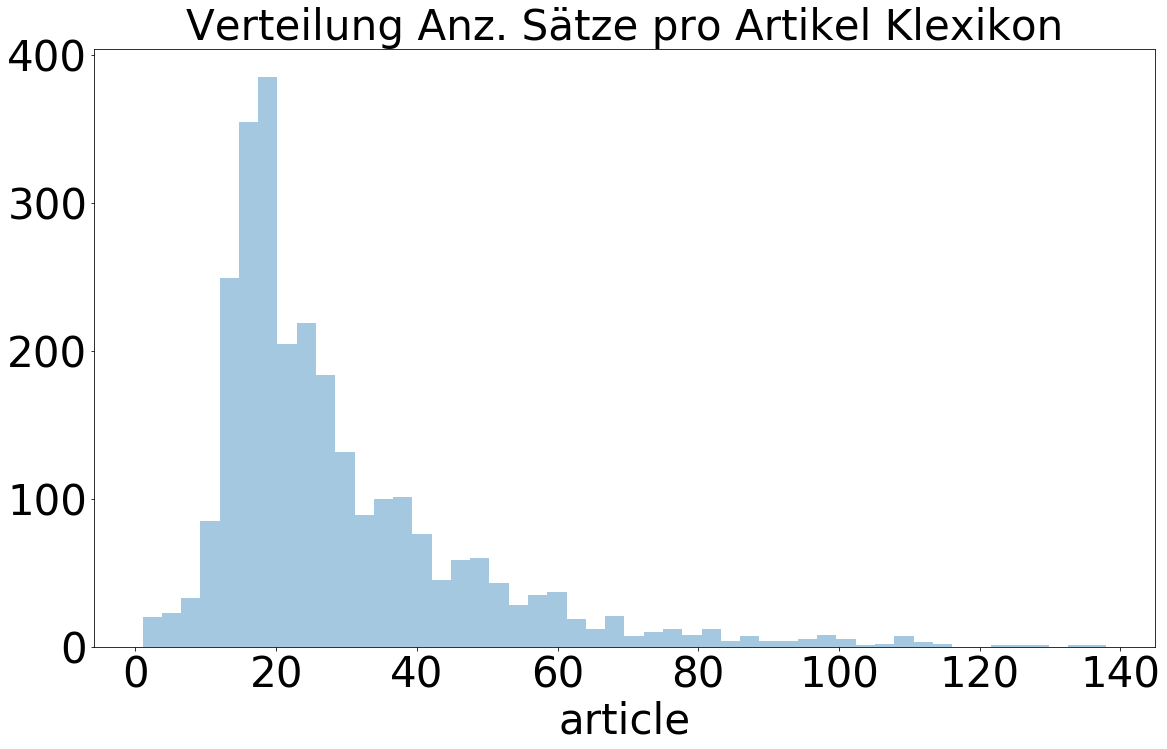
\includegraphics[width=\linewidth]{distribution_sentence_klexi.png}
    \caption{Verteilung Sätze pro Artikel Klexikon}\label{fig:distribution_sentence_klexi}
  \endminipage\hfill
  \minipage{0.45\textwidth}
    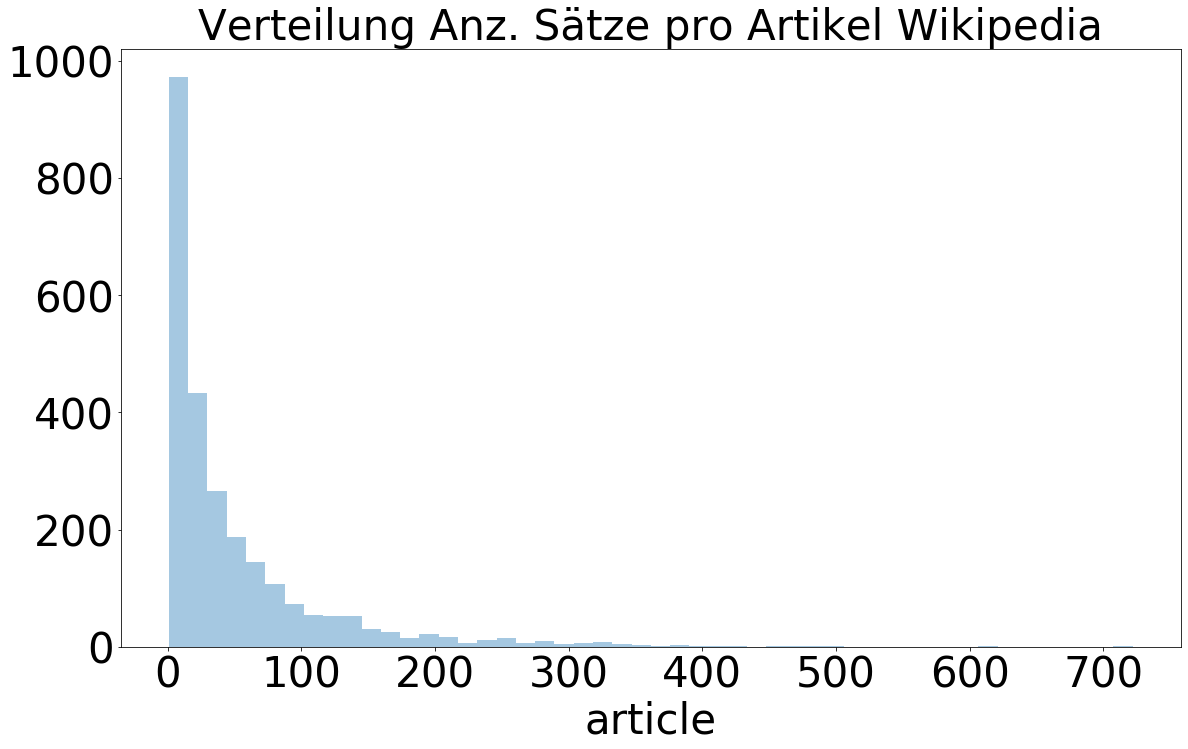
\includegraphics[width=\linewidth]{distribution_sentence_wiki.png}
    \caption{Verteilung Sätze pro Artikel Wikipedia}\label{fig:distribution_sentence_wiki}
  \endminipage\hfill     
\end{figure}
\begin{table}[H]
  \centering
  \begin{tabular}{|c|c|c|c|c|c|}
      \hline
      \textbf{Datenquelle}& \textbf{25\% Quartil}& \textbf{Median}& \textbf{75\% Quartil} & \textbf{Mean} &
      \textbf{Standardabweichung}\\
      \hline
      \textbf{Klexikon}& 17 & 23 & 35 & 28.6 & 18.3\\
      \hline
      \textbf{Wikipedia}& 8 & 24 & 63 & 49.9 & 70.0\\
      \hline
  \end{tabular}
  \caption{Verteilung der Anzahl Sätze pro Artikel für Klexikon und Wikipedia}
\label{tab:distribution_sentences_per_article}
\end{table}
\noindent
Für die Problemstellung ist jedoch die Verteilung der Anzahl Wörter in einem Satz relevant. Daher wurden Sätze mit
weniger als $ 4 $ Wörter aus dem Datensatz entfernt. Dies, da Sätze mit $ 3 $ oder weniger Wörter eine zu geringe
Relevanz für diverse Stile aufweisen. Anhand der Grafiken \ref{fig:distribution_klexi_unclean} und
\ref{fig:distribution_wiki_unclean} wird gezeigt, dass die Sätze aus Wikipedia länger gestaltet sind als die Sätze aus
dem Klexikon. Hier wird auch wie in \fullref{sec:abschliessende_problemdefinition} beschrieben, das Ziel des Style
Transfer legitimiert.
\begin{figure}[H]
  \minipage{0.45\textwidth}
    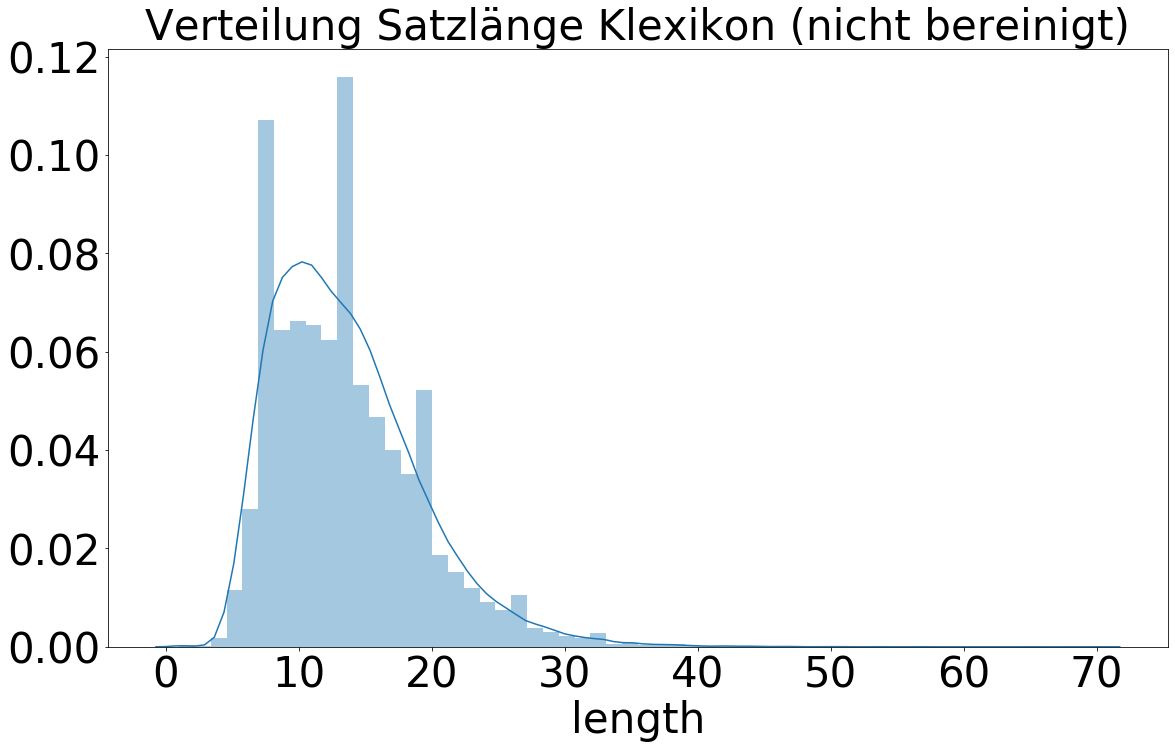
\includegraphics[width=\linewidth]{distribution_klexi_unclean.png}
    \caption{Verteilung Satzlänge Klexikon nicht bereinigt}\label{fig:distribution_klexi_unclean}
  \endminipage\hfill
  \minipage{0.45\textwidth}
    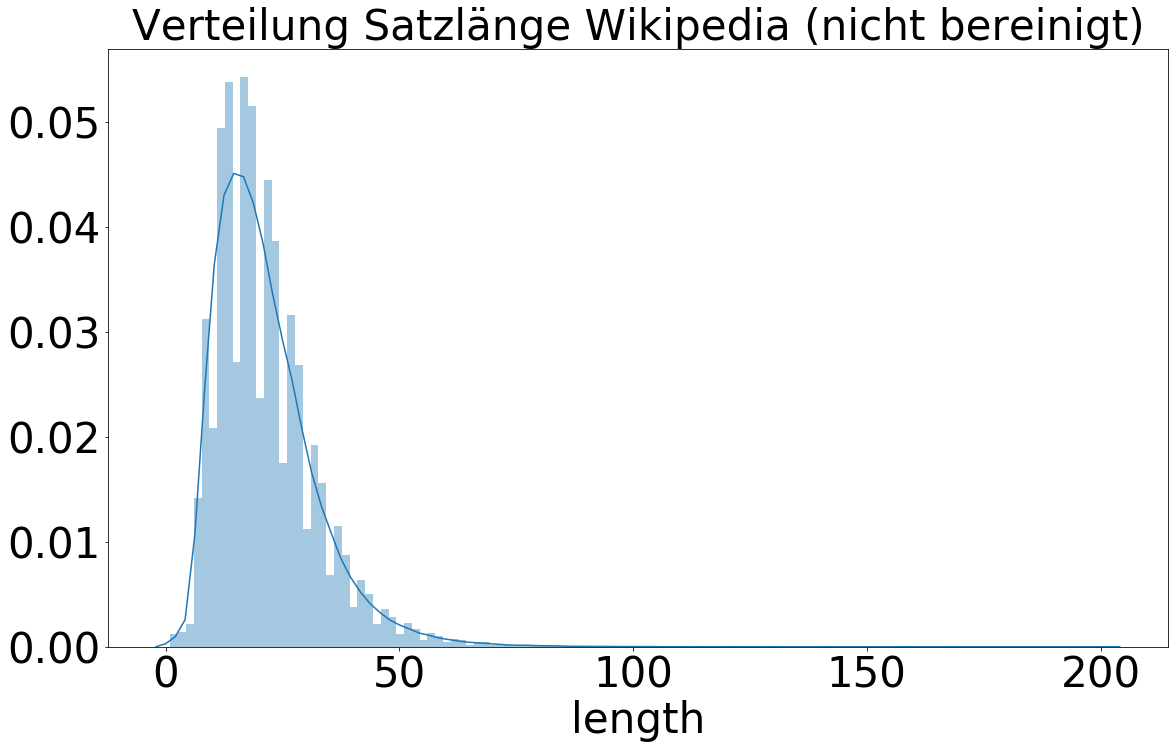
\includegraphics[width=\linewidth]{distribution_wiki_unclean.png}
    \caption{Verteilung Satzlänge Wikipedia nicht bereinigt}\label{fig:distribution_wiki_unclean}
  \endminipage\hfill     
\end{figure}
\begin{table}[H]
  \centering
  \begin{tabular}{|c|c|c|c|c|c|}
    \hline
    \textbf{Datenquelle}& \textbf{25\% Quartil}& \textbf{Median}& \textbf{75\% Quartil} & \textbf{Mean} &
    \textbf{Standardabweichung}\\
    \hline
    \textbf{Klexikon}& 9 & 13 & 17 & 13.6 & 5.5\\
    \hline
    \textbf{Wikipedia}& 14 & 19 & 27 & 21.4 & 10.8\\
    \hline
  \end{tabular}
  \caption{Verteilung Anzahl Wörter Klexikon und Wikipedia}
\label{tab:distribution_klexi_wiki_unclean}
\end{table}
\noindent
Mit Hilfe des \gls{IQR} wurden die Ausreisser aus dem Datensatz entfernt. Dabei gibt es nur Aussreisser im oberen
Bereich, da die untere Grenze unter $ 0 $ liegt. Mit der Entferung der zu kurzen Sätze, unter $ 4 $ Wörter, und Sätze
über dem oberen \gls{IQR} repräsentiert der Datenstatz weiterhin das Ziel der \fullref{sec:Problemdefinition}. Dieser
Datenbestand bildet die Basis für weitere Datensätze, siehe \fullref{sub:datensatz_ausgeglichen} und
\fullref{sub:datensatz_gekuertz}.
\begin{figure}[H]
  \minipage{0.45\textwidth}
    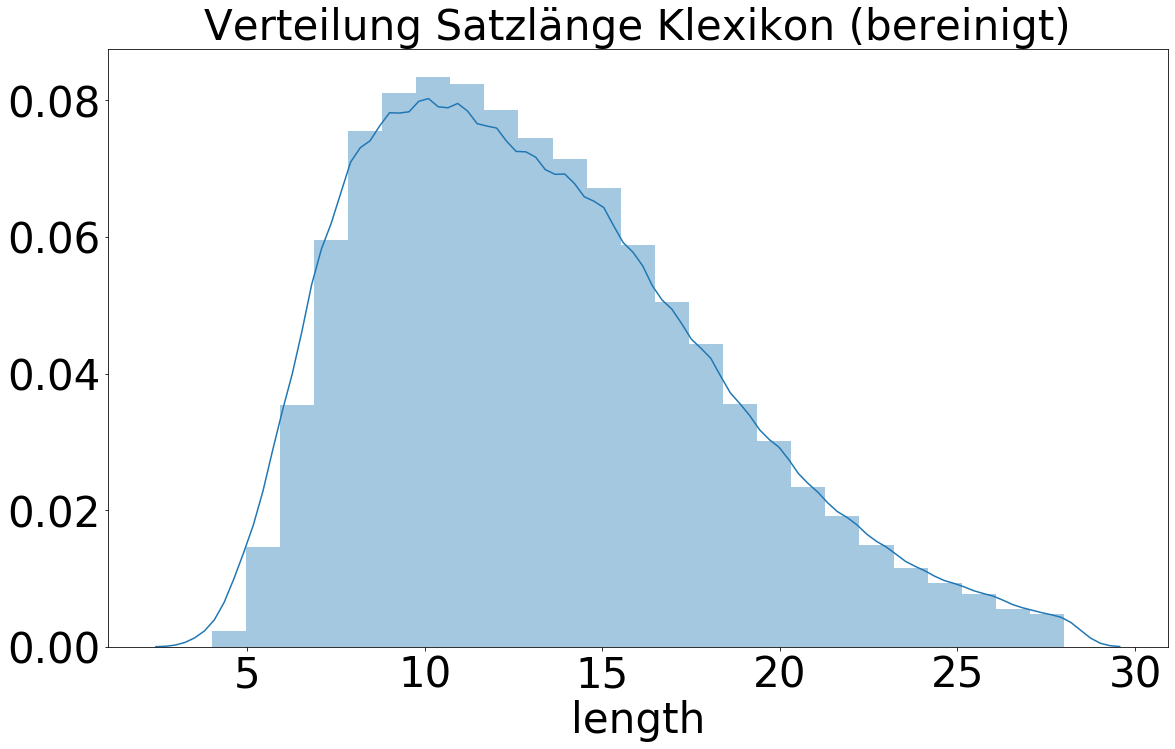
\includegraphics[width=\linewidth]{distribution_klexi_clean.png}
    \caption{Verteilung Satzlänge Klexikon bereinigt}\label{fig:distribution_klexi_clean}
  \endminipage\hfill
  \minipage{0.45\textwidth}
    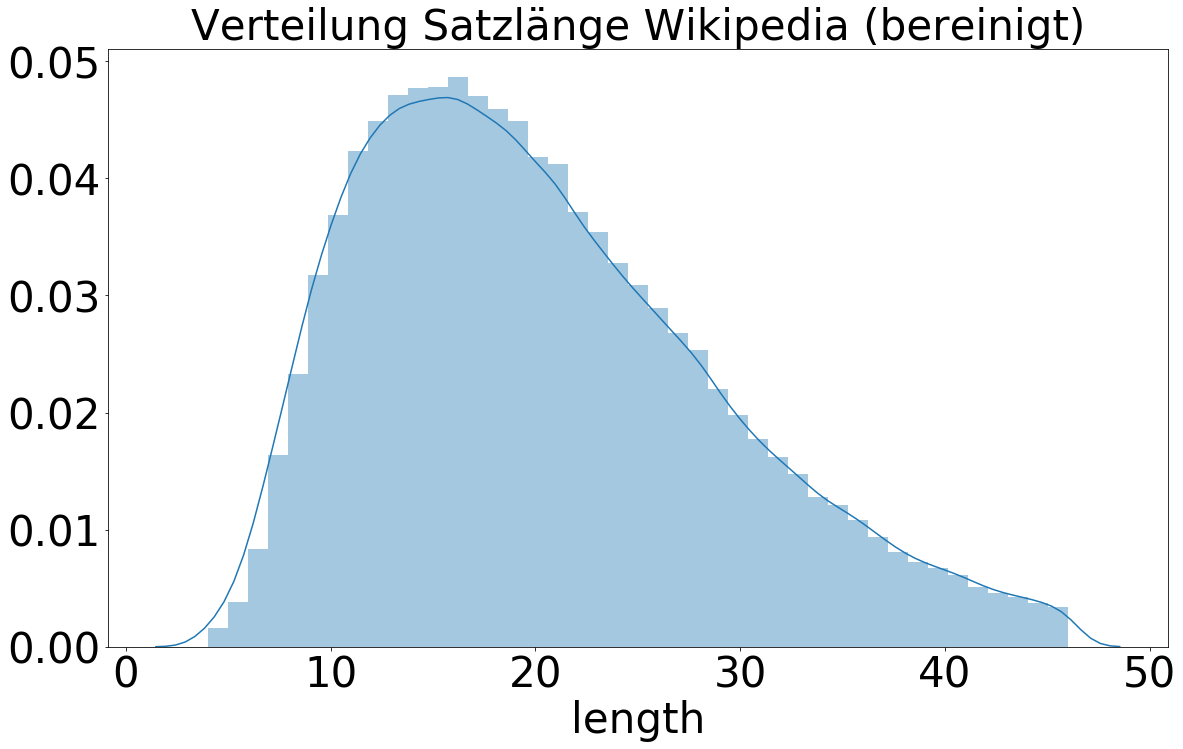
\includegraphics[width=\linewidth]{distribution_wiki_clean.png}
    \caption{Verteilung Satzlänge Wikipedia bereinigt}\label{fig:distribution_wiki_clean}
  \endminipage\hfill      
\end{figure}
\begin{table}[H]
  \centering
  \begin{tabular}{|c|c|c|c|c|c|}
    \hline
    \textbf{Datenquelle}& \textbf{25\% Quartil}& \textbf{Median}& \textbf{75\% Quartil} & \textbf{Mean} &
    \textbf{Standardabweichung}\\
    \hline
    \textbf{Klexikon}& 9 & 13 & 16 & 13.3 & 5.0\\
    \hline
    \textbf{Wikipedia}& 13 & 19 & 26 & 20.3 & 8.8\\
    \hline
  \end{tabular}
  \caption{Verteilung Anzahl Wörter Klexikon und Wikipedia ohne Ausreisser} 
\label{tab:distribution_klexi_wiki_unclean}
\end{table} 


\subsubsection{Aufbau Datensatz \flqq Ausgeglichen\frqq}
\label{sub:datensatz_ausgeglichen}
Als nächstes wurden die Grösse,  die Anzahl an Sätzen, der beide Datenquelle aneinander angepasst. Der Wikipedia
Datensatz beinhaltet ca. die doppelte Anzahl an Sätzen. Daher wurde jeder zweite Satz aus dem Wikipedia Datensatz
entfernt. Der so neu entstandene Datensatz wird wikishort genannt. In den Abbildungen
\ref{fig:article_count_ds_incl_wiki_short}, \ref{fig:sentence_count_ds_incl_wiki_short} und
\ref{fig:word_count_ds_incl_wiki_short} wird die neue Grösse der Datensätze abgebildet.
\begin{figure}[H]
  \minipage{0.32\textwidth}
    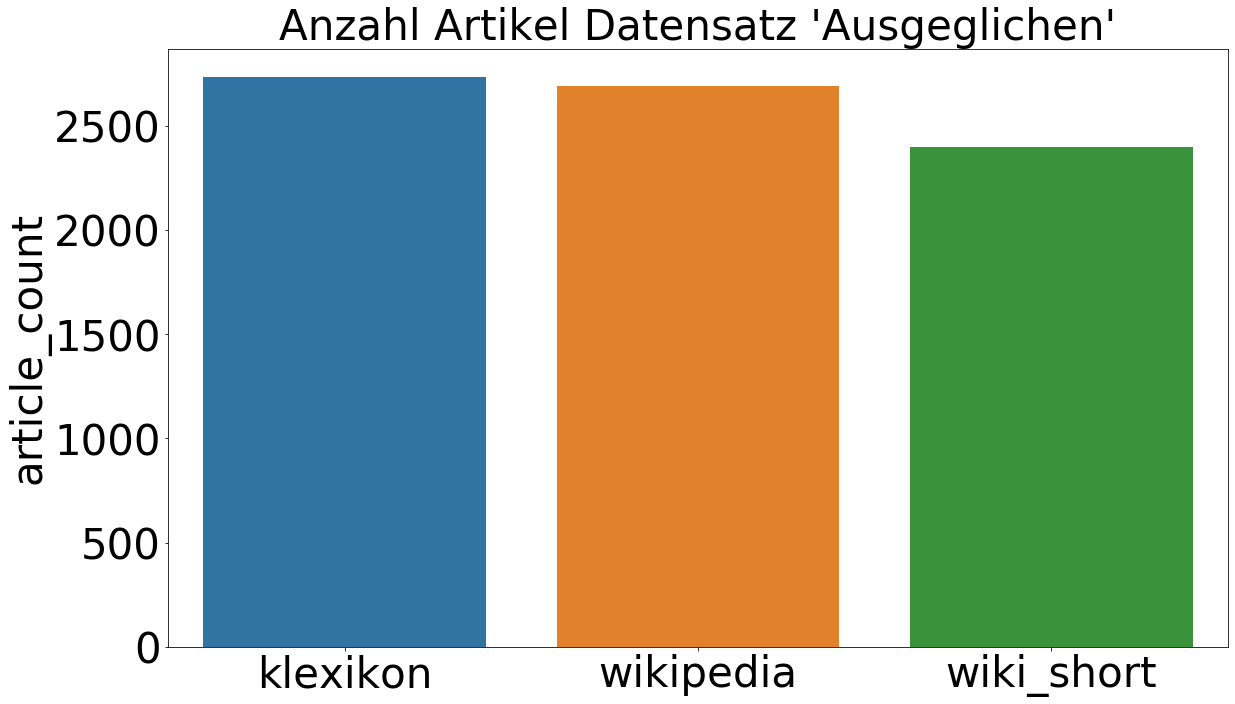
\includegraphics[width=\linewidth]{article_count_incl_wiki_short.png}
    \caption{Anz. Artikel im bereinigten Datensatz}\label{fig:article_count_ds_incl_wiki_short}
  \endminipage\hfill
  \minipage{0.32\textwidth}
    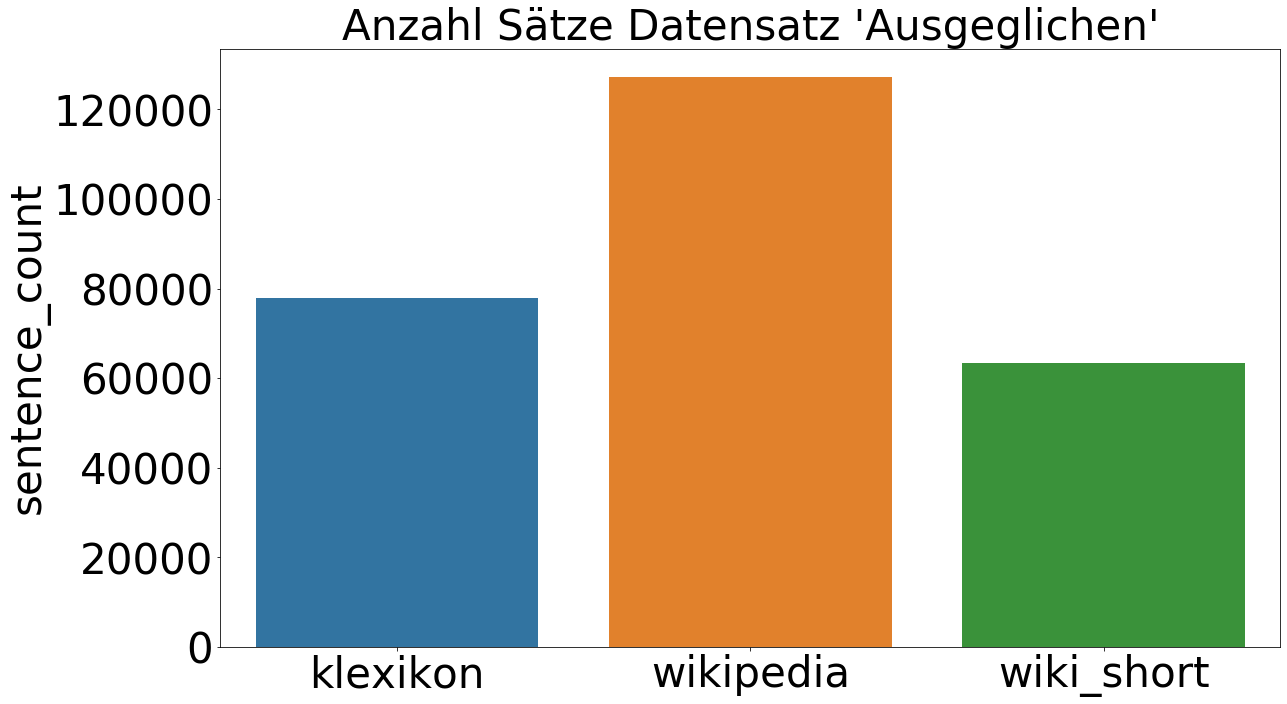
\includegraphics[width=\linewidth]{sentence_count_incl_wiki_short.png}
    \caption{Anz. Sätze im bereinigten Datensatz}\label{fig:sentence_count_ds_incl_wiki_short}
  \endminipage\hfill
  \minipage{0.32\textwidth}
    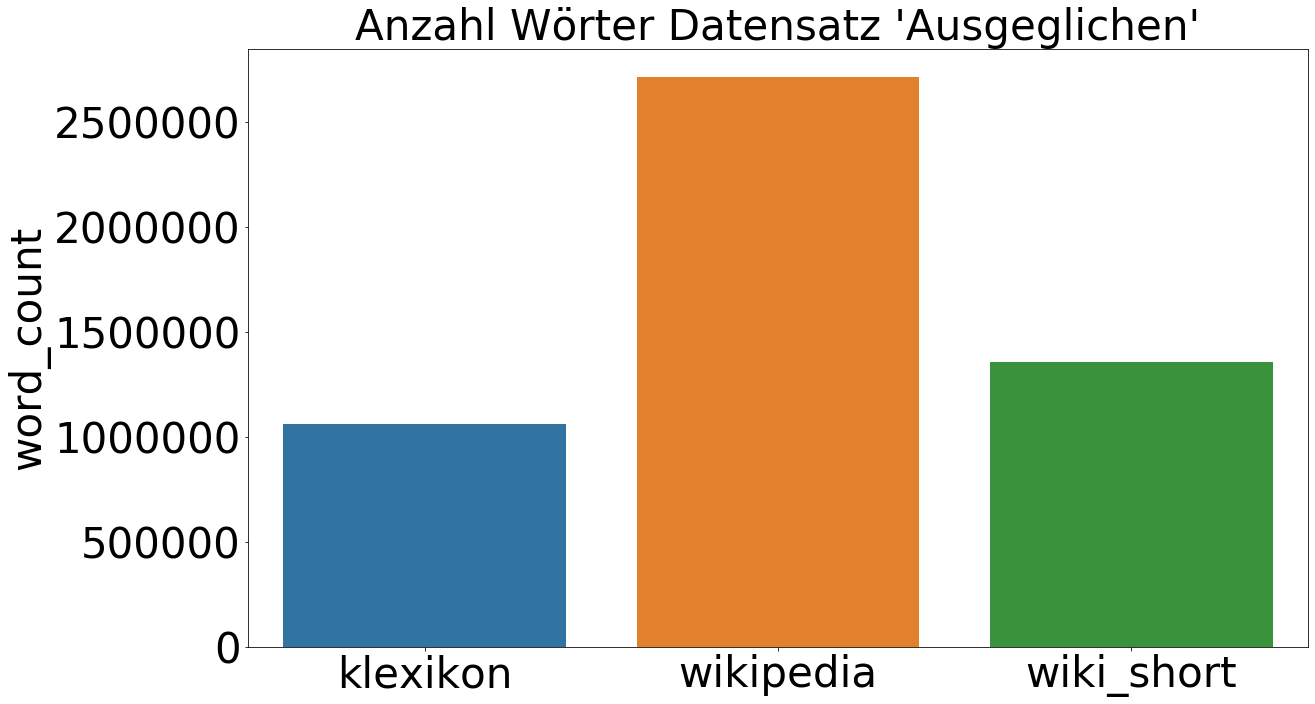
\includegraphics[width=\linewidth]{word_count_incl_wiki_short.png}
    \caption{Anz. Wörter im bereinigten Datensatz}\label{fig:word_count_ds_incl_wiki_short}
  \endminipage      
\end{figure}
\begin{table}[H]
  \centering
  \begin{tabular}{|c|c|c|c|}
      \hline
      \textbf{Datenquelle}& \textbf{Anz. Artikel}& \textbf{Anz. Sätze}& \textbf{Anz. Wörter}\\
      \hline
      \textbf{Klexikon}& 2'733 & 77'924 & 1'058'623\\
      \hline
      \textbf{Wikipedia}& 2'398 & 61'543 & 1'249'414\\
      \hline
  \end{tabular}
  \caption{Anzahl Sätze, Sätze und Wörter Klexikon, Wikipedia und Wikipedia \flqq Ausgeglichen\frqq}  
\label{tab:count_klexi_wiki_short}
\end{table}

\noindent
Da die Anzahl an Sätzen für beide Datenquellen ausgeglichen wurden, erhält dieser Datensatz die Bezeichnung \flqq
Ausgeglichen\frqq. Dies, da die Anzahl der Sätze für beide Datenquellen ausgeglichen wurden. Dabei bleibt die Verteilung
der Satzlänge auf beiden Datenquellen gleich, welches wie im Kapitel \ref{sec:abschliessende_problemdefinition}
beschrieben die Charakteristik der beiden Stile, $ erwachsen $ und $ kindlich $, beschreibt. In Abbildung
\ref{fig:distribution_both_cleaned_and_equalized} sind die beiden Verteilungen der Datenquellen noch einmal übereinander
aufgezeigt.
\begin{figure}[H]
	\centering
	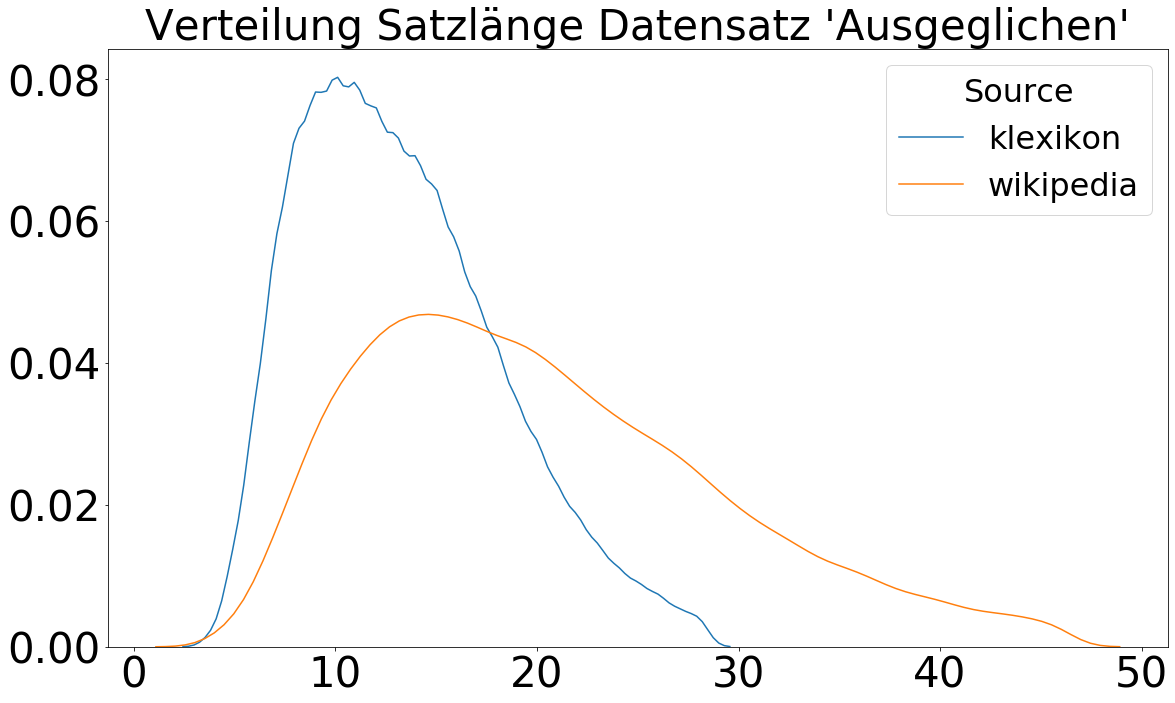
\includegraphics[scale=0.3]{distribution_both_cleaned_and_equalized.png}
	\caption{Verteilung Satzlänge Datensatz \flqq Ausgeglichen\frqq}
	\label{fig:distribution_both_cleaned_and_equalized}
\end{figure}


\subsubsection{Aufbau Datensatz \flqq Gekürzt\frqq}
\label{sub:datensatz_gekuertz}
Auf der Datenbasis des Datensatz aus \fullref{sub:statistische_analyse_des_datensatz} wurde neben dem Datensatz \flqq
Ausgeglichen\frqq, siehe \fullref{sub:datensatz_ausgeglichen}, ein zweiter Datensatz erstellt. In diesem Datensatz
sollen die beiden Stile klarer differenziert werden. Im Datensatz \flqq Ausgeglichen\frqq \ gibt es Sätze, welche sich
in der Satzlänge überschneiden. Dies soll in diesem Datensatz nicht der Fall sein. Dies bedeutet für beide Datenquellen
werden nur die Sätze verwendet die in einen gewissen Bereich fallen. Dieser Bereich soll die Stile besser definieren. Es
wurde entschieden aus der Datenquelle Klexikon nur Sätze zu verwenden, welche eine Satzlänge zwischen $ 10 $ und $ 20 $
Wörter aufweisen. Für die Datenquelle Wikipedia wurden nur Sätze, welche eine Länge zwischen $ 20 $ und $ 30 $ Wörter
enthalten. Dadurch soll ein Datensatz entstehen, in welchem die beiden Stile, welche anhand der Länge definiert werden,
klarer differenziert werden. Dieser Datensatz kann hilfreich sein, falls die Modelle die Stile aus dem Datensatz \flqq
Ausgeglichen\frqq \ nicht extrahieren kann, da die Satzlängen sich aufgrund Überschneidung zuwenig unterscheiden. Die
Verteilung der beiden Datenquelle im Datensatz \flqq Gekürzt\frqq \ sind in den Abbildungen
\ref{fig:distribution_klexi_trimmed} und \ref{fig:distribution_wiki_trimmed} zu sehen.
\begin{figure}[H]
  \minipage{0.45\textwidth}
    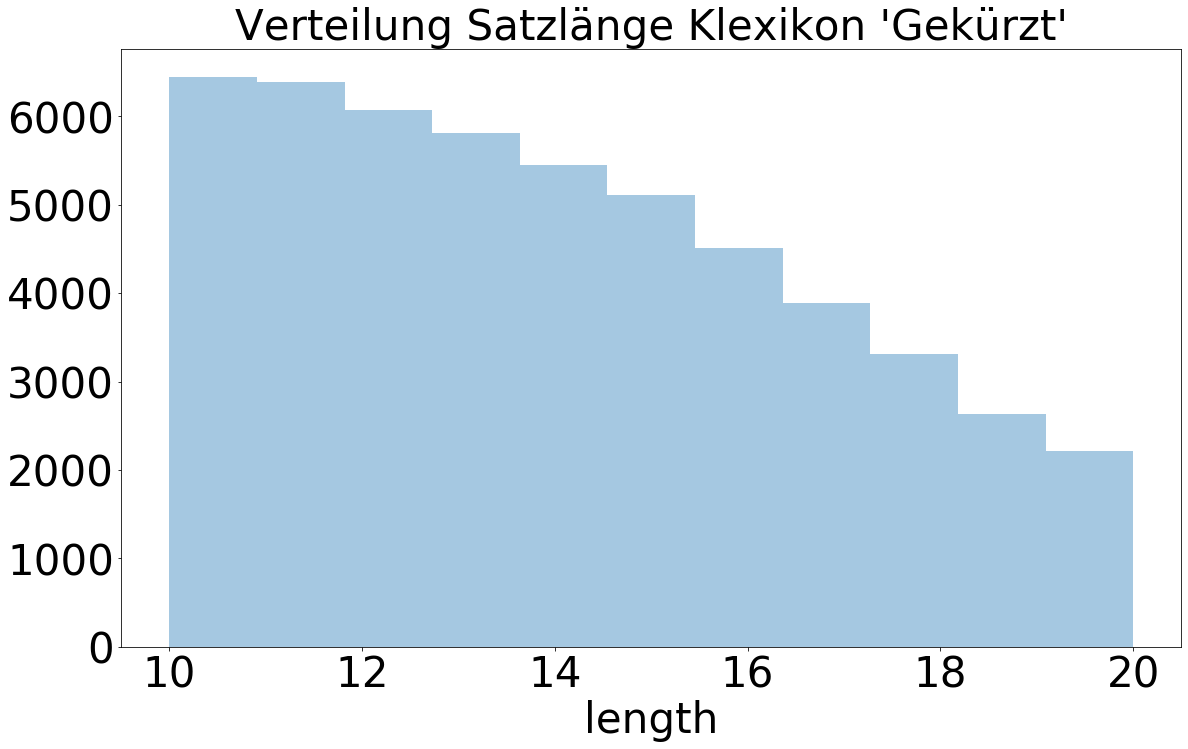
\includegraphics[width=\linewidth]{distribution_klexi_trimmed.png}
    \caption{Verteilung Satzlänge Klexikon \flqq Gekürzt\frqq}\label{fig:distribution_klexi_trimmed}
  \endminipage\hfill
  \minipage{0.45\textwidth}
    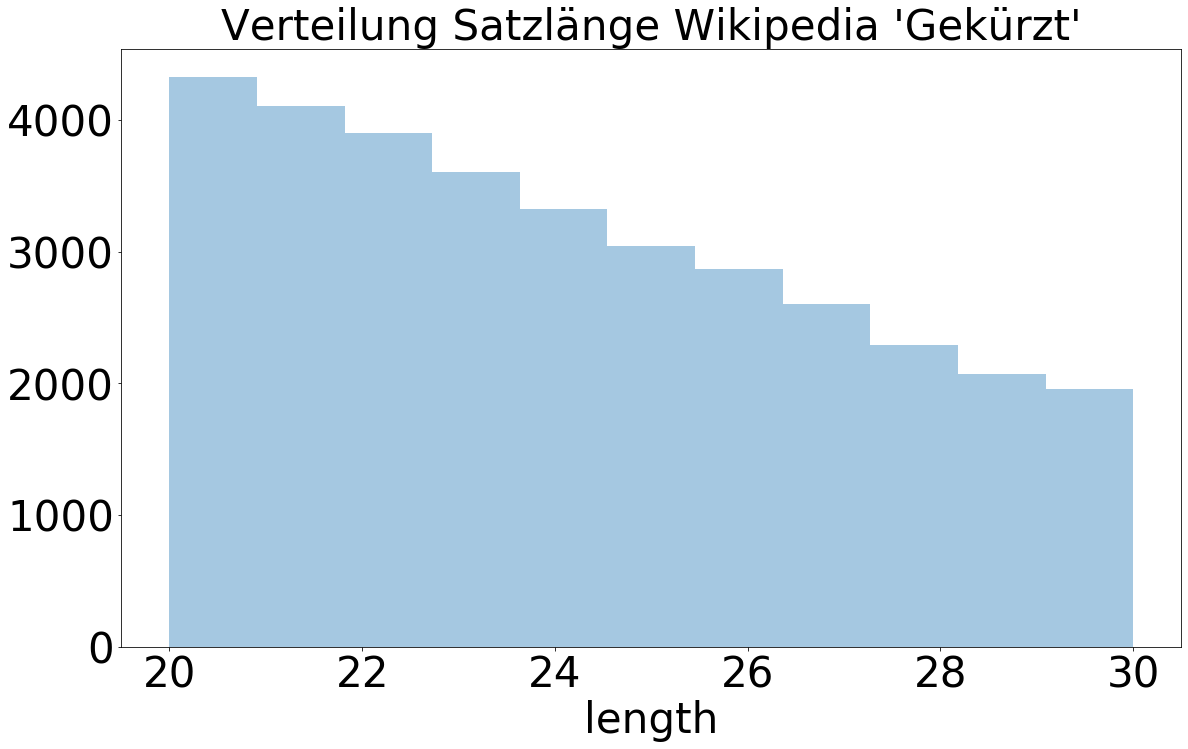
\includegraphics[width=\linewidth]{distribution_wiki_trimmed.png}
    \caption{Verteilung Satzlänge Wikipedia \flqq Gekürzt\frqq}\label{fig:distribution_wiki_trimmed}
  \endminipage\hfill
\end{figure}

\newpage

\section{Training der Modelle}
\label{sec:resultate}

Aufbauend auf den Erwähnungen in \fullref{sec:training_der_modelle} werden hier die Resultate der Modelle nach dem
Training vorgestellt. Auch sollen die Entscheidungen für die Änderungen der Hyperparameter ausgeführt werden. 
\newline
\newline
In der linken Spalte (blaue Farbe), finden sich die jeweils Resultate des Models ControlGen. In der rechten
Spalte, in Rot, sind die Resultate der CrossAlign Modelle abgebildet. Es werden drei Graphen dargestellt. Alle
Graphen zeigen die Resultate aus dem Validations Schritt des Trainings. Die erste Grafik zeigt die Genauigkeit des
durchgeführten Style Transfer. Die zweite zeigt den Verlauf der Entwicklung des \gls{BLEU} Scores für die generierten
Sätze. In der dritten Grafik wird die Verlustfunktion über die Trainingszeit dargestellt. Zum Schluss jedes Trainings
wird ein Fazit aus den Hyperparameter Einstellungen gezogen. Die Gestaltung des nächsten Trainingsdurchlauf wurde
aufgrund der Resultate der Trainings durchgeführt.

\subsection{Standard Hyperparameter}
\label{sub:standard_hyperparameter}

Zuerst wurden die beiden Modelle ControlGen und CrossAlign mit den vorgeschlagenen Hyperparameter trainiert.
Auch wurden beide Modelle auf beiden Datensätzen \flqq Ausgeglichen\frqq \ und \flqq Gekürzt\frqq \ trainiert. Die
Hyperparameter für die entsprechenden Modelle und Graphen sind in Tabelle \fullref{tab:training_standard_hyperparameter}
aufgelistet und sind im Abschnitt \ref{sub:modelle} beschrieben.
\begin{table}[ht]
	\centering
	\begin{tabular}{|l|l|l|l|l|}
    \hline
    \textbf{Hyperparameter} &
    \multicolumn{4}{c|}{\textbf{Werte}} \\
    \hline
    network & CrossAlign & CrossAlign & ControlGen & ControlGen \\
    \hline
    dataset & trimmed & equalized & trimmed & equalized \\
    \hline
    max epochs & 200 & 200 & 200 & 200 \\
    \hline
    pretrain epochs & 100 & 100 & 100 & 100 \\
    \hline
    batch size & 64 & 64 & 64 & 64 \\
    \hline
    learning rate & 0.0005 & 0.0005 & 0.0005 & 0.0005 \\
    \hline
    max len. sentences & 50 & 50 & 50 & 50 \\
    \hline
    dropout rate & 0.5 & 0.5 & 0.5 & 0.5 \\
    \hline
    number of layers & 1 & 1 & 1 & 1 \\
    \hline
    loss rec weight & 1 & 1 & 1 & 1 \\
    \hline
    trim padding & false & false & false & false \\
    \hline
    word min. occur & 3 & 3 & 3 & 3 \\
    \hline
    word embedding & embed. layer & embed.layer & embed. layer & embed. layer \\
    \hline
    dimension embedding & 100 & 100 & 100 & 100 \\
    \hline
    dimension y & 200 & 200 & 200 & 200 \\
    \hline
    dimension z & 500 & 500 & 500 & 500 \\
    \hline
    $\rho$ (rho) & 1 & 1 & 1 & 1 \\
    \hline
    $\gamma$ (gamma) & 0.1 & 0.1 & 0.1 & 0.1 \\
    \hline
    filter sizes & 1,2,3,4,5 & 1,2,3,4,5 & 1,2,3,4,5 & 1,2,3,4,5 \\
    \hline
    number of filters & 128 & 128 & 128 & 128 \\
    \hline
    \end{tabular}
	\caption{Training der Modelle mit standard Hyperparameter}
	\label{tab:training_standard_hyperparameter}
\end{table}

\subsubsection{Datensatz \flqq Ausgeglichen\frqq}

\begin{figure}[H]
  \minipage{0.45\textwidth}
    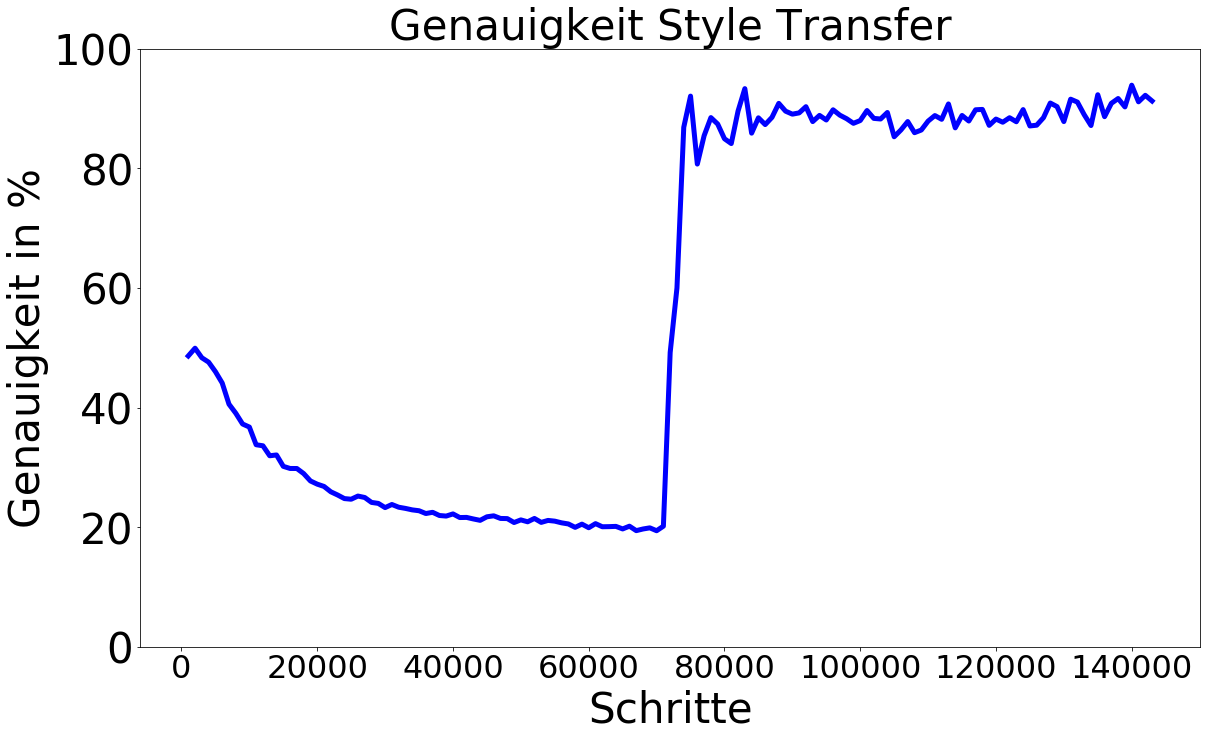
\includegraphics[width=\linewidth]{control_gen_equalized_default_full/valid_acc}
    \caption{Genauigkeit Transfer ControlGen Default \flqq Ausgeglichen\frqq}\label{fig:control_gen_equalized_default_full_valid_acc}
  \endminipage\hfill
  \minipage{0.45\textwidth}
    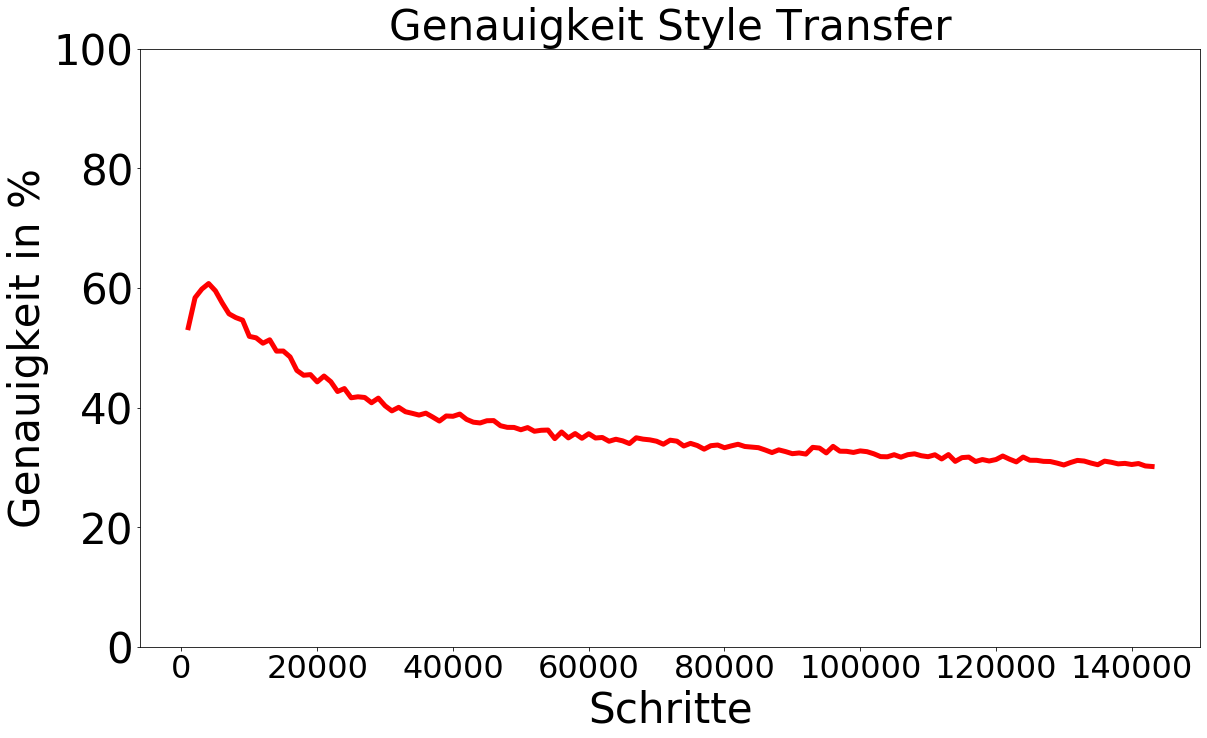
\includegraphics[width=\linewidth]{cross_align_equalized_default_full/valid_acc}
    \caption{Genauigkeit Transfer CrossAlign Default \flqq Ausgeglichen\frqq}\label{fig:cross_align_equalized_default_full_valid_acc}
  \endminipage\hfill   
\end{figure}

\begin{figure}[H]
  \minipage{0.45\textwidth}
    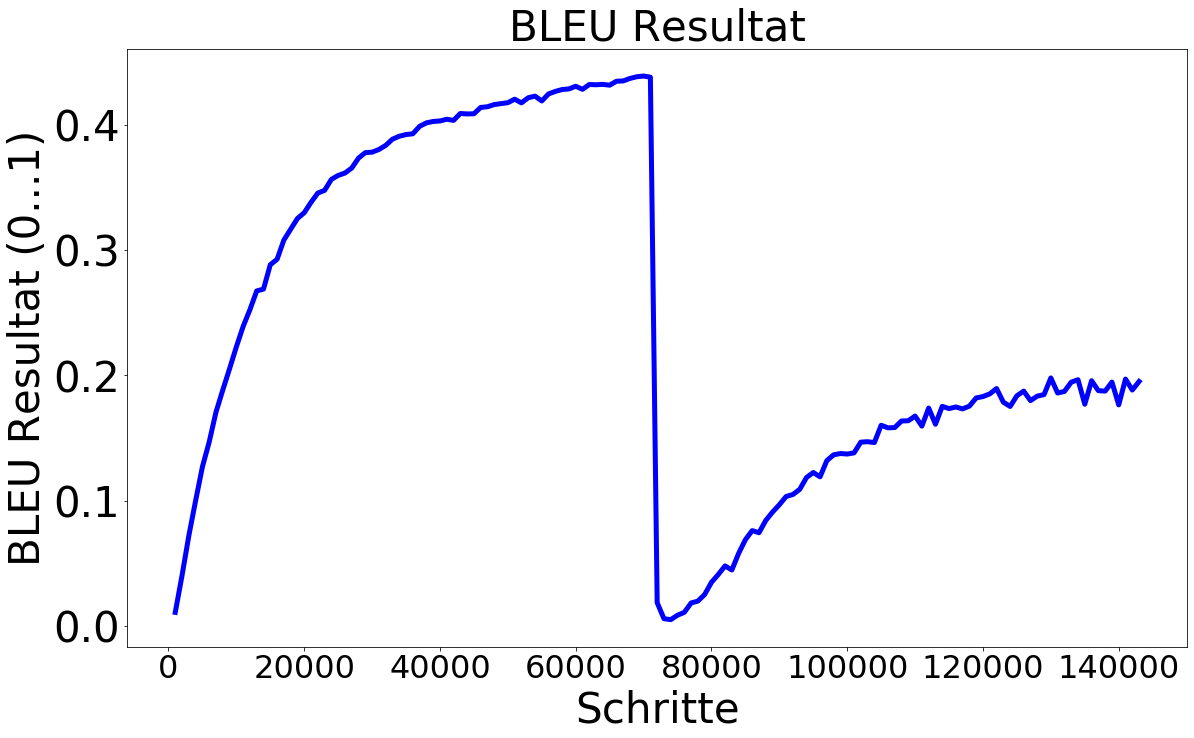
\includegraphics[width=\linewidth]{control_gen_equalized_default_full/valid_bleu}
    \caption{BLEU Score ControlGen Default \flqq Ausgeglichen\frqq}\label{fig:control_gen_equalized_default_full_valid_bleu}
  \endminipage\hfill
  \minipage{0.45\textwidth}
    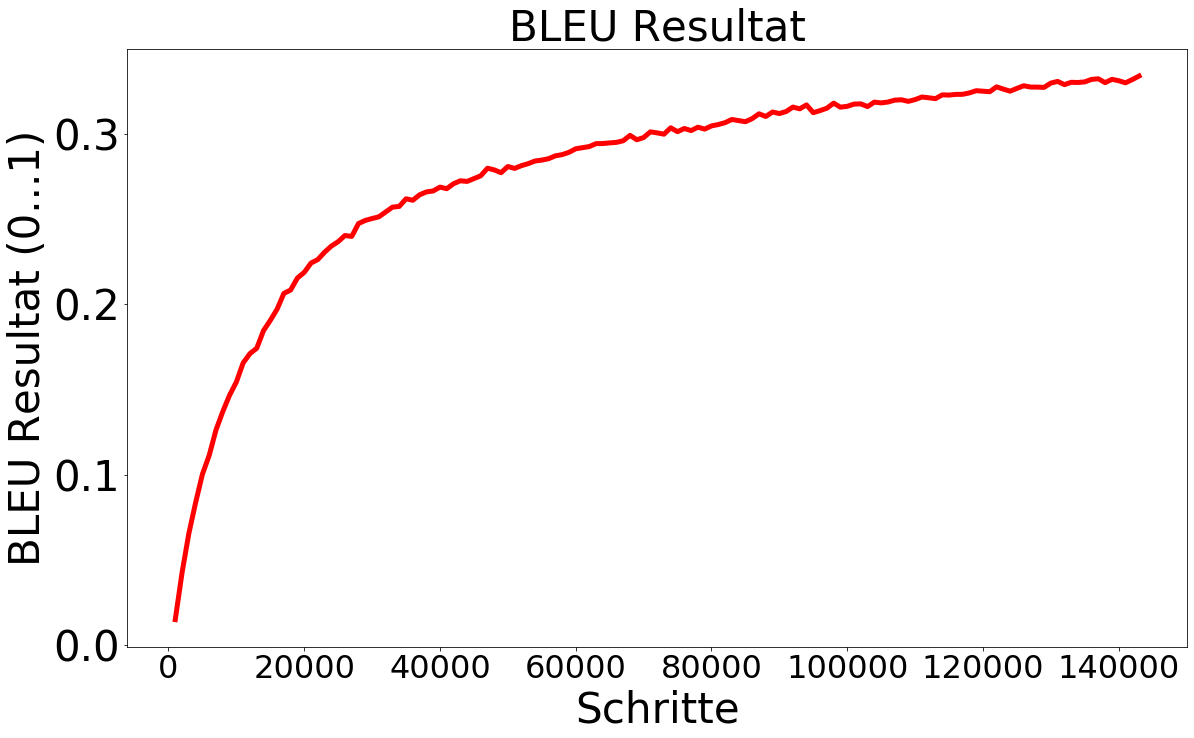
\includegraphics[width=\linewidth]{cross_align_equalized_default_full/valid_bleu}
    \caption{BLEU Score Transfer CrossAlign Default \flqq Ausgeglichen\frqq}\label{fig:cross_align_equalized_default_full_valid_bleu}
  \endminipage\hfill   
\end{figure}

\begin{figure}[H]
  \minipage{0.45\textwidth}
    \includegraphics[width=\linewidth]{control_gen_equalized_default_full/valid_loss}
    \caption{Verlustfunktion ControlGen Default \flqq Ausgeglichen\frqq}\label{fig:control_gen_equalized_default_full_valid_loss}
  \endminipage\hfill
  \minipage{0.45\textwidth}
    \includegraphics[width=\linewidth]{cross_align_equalized_default_full/valid_loss}
    \caption{Verlustfunktion CrossAlign Default \flqq Ausgeglichen\frqq}\label{fig:cross_align_equalized_default_full_valid_loss}
  \endminipage\hfill   
\end{figure}
\noindent

\subsubsection{Datensatz \flqq Gekürzt\frqq}

\begin{figure}[H]
  \minipage{0.45\textwidth}
    \includegraphics[width=\linewidth]{control_gen_trimmed_default_full/valid_acc}
    \caption{Genauigkeit Transfer ControlGen Default \flqq Gekürzt\frqq}\label{fig:control_gen_trimmed_default_full_valid_acc}
  \endminipage\hfill
  \minipage{0.45\textwidth}
    \includegraphics[width=\linewidth]{cross_align_trimmed_default_full/valid_acc}
    \caption{Genauigkeit Transfer CrossAlign Default \flqq Gekürzt\frqq}\label{fig:cross_align_trimmed_default_full_valid_acc}
  \endminipage\hfill   
\end{figure}

\begin{figure}[H]
  \minipage{0.45\textwidth}
    \includegraphics[width=\linewidth]{control_gen_trimmed_default_full/valid_bleu}
    \caption{BLEU Score ControlGen Default \flqq Gekürzt\frqq}\label{fig:control_gen_trimmed_default_full_valid_bleu}
  \endminipage\hfill
  \minipage{0.45\textwidth}
    \includegraphics[width=\linewidth]{cross_align_trimmed_default_full/valid_bleu}
    \caption{BLEU Score Transfer CrossAlign Default \flqq Gekürzt\frqq}\label{fig:cross_align_trimmed_default_full_valid_bleu}
  \endminipage\hfill   
\end{figure}

\begin{figure}[H]
  \minipage{0.45\textwidth}
    \includegraphics[width=\linewidth]{control_gen_trimmed_default_full/valid_loss}
    \caption{Verlustfunktion ControlGen Default \flqq Gekürzt\frqq}\label{fig:control_gen_trimmed_default_full_valid_loss}
  \endminipage\hfill
  \minipage{0.45\textwidth}
    \includegraphics[width=\linewidth]{cross_align_trimmed_default_full/valid_loss}
    \caption{Verlustfunktion CrossAlign Default \flqq Gekürzt\frqq}\label{fig:cross_align_trimmed_default_full_valid_loss}
  \endminipage\hfill   
\end{figure}

\subsubsection{Fazit der Hyperparameter Einstellungen}

Wie in Abbildung \ref{fig:cross_align_equalized_default_full_valid_acc} und
\ref{fig:cross_align_trimmed_default_full_valid_acc} ersichtlich wird kann der Style Transfer mit dem Modell
CrossAlign nicht richtig durchgeführt werden. Dies ist aufgrund der sich nicht ändernden Genauigkeit des Transfers
zu erklären. Obwohl der \gls{BLEU} Score für den Datensatz \flqq Ausgeglichen\frqq \ höher aus fällt als für den
Datensatz \flqq Gekürzt\frqq, siehe \ref{fig:control_gen_equalized_default_full_valid_bleu},
\ref{fig:cross_align_equalized_default_full_valid_bleu}, \ref{fig:control_gen_trimmed_default_full_valid_bleu},
\ref{fig:cross_align_trimmed_default_full_valid_bleu}. Aufgrund der transferierten Sätze, siehe Repository
\fullref{sub:wipro-logs}, ist ersichtlich, dass die Länge der Sätze dabei jedoch nicht ändert. Da die Satzlängen sich
nicht ändern kann auch der hohe \gls{BLEU} Score erklärt werden, siehe \fullref{sub:BLEU}. Dies bestätigt Teilweise die
Vermutung, der sich zu stark überschneidenden Sätze, siehe \fullref{sec:aufbau_datensatz}. Daher wurde nach der Sichtung
der transferierten Sätze entschieden, die weiteren Trainings nur noch auf dem Datensatz \flqq Gekürzt\frqq \
durchzuführen. 
\newline
\newline
Die Verlustfunktion, \ref{fig:control_gen_equalized_default_full_valid_loss} und
\ref{fig:cross_align_equalized_default_full_valid_loss}, setzt sich aus der Verlustfunktion für die Diskriminatoren und
Generatoren zusammen, siehe Repository \fullref{sub:gan}. In Absprache mit der Betreuungsperson wurden daher für
den nächsten Trainingsdurchlauf entschieden, eine gewichtete Funktion auszuprobieren. Dies, da der Verlust des
Transfers einen grossen Einfluss auf den gesamt Verlust hat.

\newpage

\subsection{Standard Hyperparameter mit gewichteter Verlustfunktion}
\label{sub:weighted_hyperparameter}

In diesem Trainingsdurchlauf wurde die gewichtete Verlustfunktion für den Transfer Verlust eingefügt. Die
Hyperparameter wurde auf den Standardwerten belassen, dies um einen Vergleich zum Training ohne gewichtete
Verlustfunktionen zu erhalten. Diese Einstellungen wurden nur noch auf dem Datensatz \flqq Gekürzt\frqq \ durchgeführt.
Die Hyperparameter für die entsprechenden Modelle und Graphen sind in Tabelle
\fullref{tab:training_weighted_loss_hyperparameter} aufgelistet und sind im Abschnitt \ref{sub:modelle} beschrieben.
\begin{table}[ht]
	\centering
	\begin{tabular}{|l|l|l|}
    \hline
    \textbf{Hyperparameter} &
    \multicolumn{2}{c|}{\textbf{Werte}} \\
    \hline
    network & CrossAlign & ControlGen \\
    \hline
    dataset & trimmed & trimmed \\
    \hline
    max epochs & 200 & 200 \\
    \hline
    pretrain epochs & 100 & 100 \\
    \hline
    batch size & 64 & 64 \\
    \hline
    learning rate & 0.0005 & 0.0005 \\
    \hline
    max len. sentences & 50 & 50 \\
    \hline
    dropout rate & 0.5 & 0.5 \\
    \hline
    number of layers & 1 & 1 \\
    \hline
    loss rec weight & 0.5 & 0.5 \\
    \hline
    trim padding & false & false \\
    \hline
    word min. occur & 3 & 3 \\
    \hline
    word embedding & embed. layer & embed. layer \\
    \hline
    dimension embedding & 100 & 100 \\
    \hline
    dimension y & 200 & 200 \\
    \hline
    dimension z & 500 & 500 \\
    \hline
    $\rho$ (rho) & 1 & 1 \\
    \hline
    $\gamma$ (gamma) & 0.1 & 0.1 \\
    \hline
    filter sizes & 1,2,3,4,5 & 1,2,3,4,5 \\
    \hline
    number of filters & 128 & 128 \\
    \hline
    \end{tabular}
	\caption{Training der Modelle mit gewichteter Transfer Lossfunktion Hyperparameter}
	\label{tab:training_weighted_loss_hyperparameter}
\end{table}

\begin{figure}[H]
  \minipage{0.45\textwidth}
    \includegraphics[width=\linewidth]{control_gen_trimmed_new_loss_full/valid_acc}
    \caption{Genauigkeit Transfer ControlGen Gewichtet \flqq Gekürzt\frqq}\label{fig:control_gen_trimmed_new_loss_full_valid_acc}
  \endminipage\hfill
  \minipage{0.45\textwidth}
    \includegraphics[width=\linewidth]{cross_align_trimmed_new_loss_full/valid_acc}
    \caption{Genauigkeit Transfer CrossAlign Gewichtet \flqq Gekürzt\frqq}\label{fig:cross_align_trimmed_new_loss_full_valid_acc}
  \endminipage\hfill   
\end{figure}

\begin{figure}[H]
  \minipage{0.45\textwidth}
    \includegraphics[width=\linewidth]{control_gen_trimmed_new_loss_full/valid_bleu}
    \caption{BLEU Score ControlGen Gewichtet \flqq Gekürzt\frqq}\label{fig:control_gen_trimmed_default_new_loss_valid_bleu}
  \endminipage\hfill
  \minipage{0.45\textwidth}
    \includegraphics[width=\linewidth]{cross_align_trimmed_new_loss_full/valid_bleu}
    \caption{BLEU Score Transfer CrossAlign Gewichtet \flqq Gekürzt\frqq}\label{fig:cross_align_trimmed_new_loss_full_valid_bleu}
  \endminipage\hfill   
\end{figure}

\begin{figure}[H]
  \minipage{0.45\textwidth}
    \includegraphics[width=\linewidth]{control_gen_trimmed_new_loss_full/valid_loss}
    \caption{Verlustfunktion ControlGen Gewichtet \flqq Gekürzt\frqq}\label{fig:control_gen_trimmed_new_loss_full_valid_loss}
  \endminipage\hfill
  \minipage{0.45\textwidth}
    \includegraphics[width=\linewidth]{cross_align_trimmed_new_loss_full/valid_loss}
    \caption{Verlustfunktion CrossAlign Gewichtet \flqq Gekürzt\frqq}\label{fig:cross_align_trimmed_new_loss_full_valid_loss}
  \endminipage\hfill   
\end{figure}

\subsubsection{Fazit der Hyperparameter Einstellungen}
Die Resultate des Trainings \fullref{sub:weighted_hyperparameter} sind nahezu identisch mit
\fullref{sub:standard_hyperparameter}. Daraus kann die Verbesserung der Modelle mit einer Gewichtung des Transfer
Verlust nicht erreicht werden. Weiter wurde nach diesem Trainingsdurchlauf entschieden, weitere Trainings nur noch auf
dem ControlGen Modell durchzuführen. Dies ist aufgrund der sich nicht ändernden Genauigkeit des Transfers. In
\ref{fig:control_gen_trimmed_new_loss_full_valid_acc} und \ref{fig:cross_align_trimmed_new_loss_full_valid_acc} ist
ersichtlich dass, das Modell CrossAlign den Style Transfer nicht wie gewünscht durchführt. 

\newpage

\subsection{ControlGen mit grösseren Dimensionen}
\label{sub:bigger_embedding_hyperparameter}

Da der \gls{BLEU} Score für die ControlGen Modelle niedrig ausfällt, wurde entschieden, die Dimension für das Word
Embedding, sowie den Kontext und Style Raum zu vergrössern. Dadurch hat das Modell mehr Variablen für das Training zur
Verfügung. Damit das Modell trainiert werden kann ist mehr \gls{RAM} auf der Grafikkarte nötig. Daher wurde für dieses
Training eine Grafikkarte mit 32GB \gls{RAM}, NVIDIA Tesla 100V, verwendet. Die Hyperparameter für die entsprechenden
Modelle und Graphen sind in Tabelle \fullref{tab:training_big_embedding_hyperparameter} aufgelistet und sind im
Abschnitt \ref{sub:modelle} beschrieben.
\begin{table}[ht]
	\centering
	\begin{tabular}{|l|l|}
    \hline
    \textbf{Hyperparameter} &
    \textbf{Werte} \\
    \hline
    network  & ControlGen \\
    \hline
    dataset  & trimmed \\
    \hline
    max epochs & 200 \\
    \hline
    pretrain epochs & 100 \\
    \hline
    batch size & 64 \\
    \hline
    learning rate & 0.0005 \\
    \hline
    max len. sentences & 50 \\
    \hline
    dropout rate & 0.5 \\
    \hline
    number of layers & 1 \\
    \hline
    loss rec weight & 1 \\
    \hline
    trim padding & false \\
    \hline
    word min. occur & 3 \\
    \hline
    word embedding & embed. layer \\
    \hline
    dimension embedding & 300 \\
    \hline
    dimension y & 300 \\
    \hline
    dimension z & 900 \\
    \hline
    $\rho$ (rho) & 1 \\
    \hline
    $\gamma$ (gamma) & 0.1 \\
    \hline
    filter sizes & 1,2,3,4,5 \\
    \hline
    number of filters & 128 \\
    \hline
    \end{tabular}
	\caption{Training der Modelle mit grösseren Embedding Hyperparametern}
	\label{tab:training_big_embedding_hyperparameter}
\end{table}

\begin{figure}[H]
    \centering
    \includegraphics[scale=0.25]{control_gen_trimmed_bigger_embedding_full/valid_acc}
    \caption{Genauigkeit Transfer ControlGen Dimensionen \flqq Gekürzt\frqq}\label{fig:control_gen_trimmed_bigger_embedding_full_valid_acc}
\end{figure}

\begin{figure}[H]
    \centering
    \includegraphics[scale=0.25]{control_gen_trimmed_bigger_embedding_full/valid_bleu}
    \caption{BLEU Score ControlGen Dimensionen \flqq Gekürzt\frqq}\label{fig:control_gen_trimmed_bigger_embedding_full_valid_bleu}
\end{figure}

\begin{figure}[H]
    \centering
    \includegraphics[scale=0.25]{control_gen_trimmed_bigger_embedding_full/valid_loss}
    \caption{Verlustfunktion ControlGen Dimensionen \flqq Gekürzt\frqq}\label{fig:control_gen_trimmed_bigger_embedding_full_valid_loss}
\end{figure}

\subsubsection{Fazit der Hyperparameter Einstellungen}
Wie erwartet, konnte der \gls{BLEU} Score mit einem grösseren Raum verbessert werden. Dies jedoch nur in der
Trainingsphase des Vortrainings, siehe \fullref{sub:control_gen}. Die transferierten Sätze sind jedoch auch mit diesen
Trainingseinstellungen nicht zufriedenstellend. Auf eine weitere Erhöhung der Dimensionen wurde aufgrund von Zeit- und
Ressourcenmangel verzichtet. Zu diesem Zeitpunkt im Projekt wurde entschieden auf weitere Trainings zu verzichten. Es
scheint so, dass mit dem verwendeten Modellen kein zufriedenstellendes Resultat erreichen werden kann. Begründungen für
diese Annahme werden in \fullref{ch:Eval} aufgeführt.

\section{Prototyp}
\label{sec:prototyp}
Um die einzelnen Modelle auch mit einem beliebigen Eingabesatz zu testen wurde ein Prototyp in Python (\cite{python})
entwickelt, welcher ein gewisses Modell laden kann und anschliessend einen eingegebenen Satz in einen anderen
transferiert.
\newline
\newline
Der Prototyp wurde aus zeitlichen Gründen ohne User Interface entwickelt und ist daher ein Python Skript mit einem
Command Line Interface. Die Umsetzung wurde bewusst sehr minimal gehalten, da der Fokus dieser Arbeit mehrheitlich auf
dem Erarbeiten vielversprechender Modelle war anstatt auf der Entwicklung eines erweiterten Prototypen. Dies wurde
aufgrund der dürftigen Ergebnisse der trainierten Modelle entschieden.
\newline
\newline
Um die Benutzung und Installation des Prototypen zu erleichtern wurde ein Docker Image (\cite{docker}) geschrieben,
welches als erstes Git herunterlädt, um das \fullref{sub:wipro-source} Git klonen zu können. Anschliessend werden die
PIP Requirements des Projektes installiert so dass alles korrekt funktioniert. Bei jedem ausführen des Containers wird
der Prototyp direkt ausgeführt, so dass dieser benutzt werden kann ohne weitere Schritte. Das Docker Image wurde auf
Docker Hub (\cite{docker_hub}) geladen, so dass dieses wie ein Git Repository, heruntergeladen werden kann. Dieses Image
ist unter der URL \hyperlink{https://hub.docker.com/repository/docker/fabiangroeger96/wipro-prototype}{Docker Image
Prototype} erreichbar und ist öffentlich. Das Dockerfile um das Docker Image zu erstellen befindet sich im
\fullref{sub:wipro-source} Projekt.
\newline
\newline
Wenn das Docker Image ausgeführt wird, startet sogleich der Prototyp. Als Erstes wird nach dem Modell, welches für den
Style Transfer gebraucht wird, gefragt. Dabei stehen drei verschiedene zur Verfügung:
\begin{enumerate}
  \setlength\itemsep{0em}
  \item \textbf{cross-align-trimmed-new-loss-full}, ein \fullref{sub:cross_align} Netzwerk trainiert auf dem \flqq
  wipro-trimmed\frqq \ Datensatz über 200 Epochen mit den default Hyperparametern, \fullref{sub:standard_hyperparameter}
  \item \textbf{control-gen-trimmed-bigger-embedding-full}, ein \fullref{sub:control_gen} Netzwerk trainiert auf dem \flqq
  wipro-trimmed\frqq \ Datensatz über 200 Epochen mit den Hyperparametern für ein grösseres Embedding,
  \fullref{sub:bigger_embedding_hyperparameter}
  \item \textbf{control-gen-equalized-default-full}, ein \fullref{sub:control_gen} trainiert auf dem \flqq
  wipro-trimmed\frqq \ Datensatz über 200 Epochen mit den default Hyperparametern, \fullref{sub:standard_hyperparameter}
\end{enumerate}
\noindent
Nach dem Eingeben der Nummer des gewünschten Modells wird das Modell initialisiert und anschliessend die gespeicherten
Gewichte geladen, dieser Prozess kann je nach Computer etwas länger dauern. Als Nächstes kann ein Satz zum Transfer
eingegeben werden. Dieser wird anschliessend zu einem Batch hinzugefügt und dem Modell übergeben. Der eine Output ist
danach der transferierte Satz, welcher noch aus einem encodierten Vektor der Wörter besteht. Diesen kann man anhand des
Vokabulars des Modells in Wörter zurückmappen. Als zweiter Output ist der rekonstruierte Satz, welcher auch mittels dem
Vokabular zurück transferiert wird. Diese beiden Sätze werden anschliessend ausgegeben und dargestellt.

\begin{figure}[H]
  \centering
  \includegraphics[scale=0.275]{prototyp}
  \caption{Command Line Interface des Prototypen}\label{fig:prototyp}
\end{figure}


\chapter{Evaluation und Validation}
\label{ch:Eval}

In diesem Kapitel werden die Resultate der Modelle wie in \ref{sec:method_eval} beschrieben evaluiert. Zuerst wird darauf
eingegangen wie die Resultate der Modelle evaluiert werden. Weiter wird aufgeführt welche Anforderungen erreicht werden
sollten. Anschliessend wird die eigentliche Evaluation durchgeführt.

\section{Vorgehen der Evaluierung}
\label{sec:vorgehen_evaluation}

Wie bereits in \ref{sec:method_eval} beschrieben wird soll die Verteilung der Satzlänge der Ausgangssätze sowie den
Zielsätzen verglichen werden. Wie auch in \ref{sub:statistische_analyse_des_datensatz} aufgeführt werden die Stillabel $
wikipedia $ und $ klexikon $ durch ihre Satzlänge unterschieden. Für die Evaluierung wird auf den Validationsteil des
Datensatzes ein Transfer durchgeführt. Dabei werden die Sätze aus dem Stillabel $ wikipedia $ in einen Satz aus dem
Stillabel $ klexikon $ transferiert. Entsprechendes gilt für die Sätze aus dem Label $ klexikon $, welche in einen Satz
aus dem Stillabel $ wikipedia $ gewandelt werden. Für das erreichen der Anforderungen ist vorallem die Wandlung
von kürzeren Sätzen in das Labels $ klexikon $ interessant. Dies da es sich bei den Zielen der Aufgabenstellung,
\ref{sec:Aufgabenstellung-Zielsetzung}, ebenfalls um einen Transfer handelt welche eine längere Satzlänge fordert.
\newline
\newline
Um die Verteilung er Satzlängen aus den Stillabels zu vergleichen werden ca. $ 15'000 $ Sätze aus jedem Stillabel einem
Transfer unterzogen. Anschliessend werden die Anzahl Wörter des Eingabesatzes sowie des entsprechenden Ausgabesatz
verglichen. Anschliessend wird die Differenz der Länge der beiden Sätze gebildet. Es wird erwartet das der Durchschnitt
der Differenz für die Ausgabesätze grösser $ 0 $ entspricht.
\newline
\newline
Aufgrund der Resultate in \ref{sec:resultate} wurde entschieden das letzte Modell
\fullref{sub:bigger_embedding_hyperparameter} zu evaluieren. Um ebenfalls einen Vergleich zwischen den beiden Modelle
ControlGen und CrossAlign zu erhalten, wird ebenfalls das CrossAlign Modell aus
\ref{sub:weighted_hyperparameter} mit der beschriebenen Methode evaluiert. Beide evaluierten Modelle wurden auf dem
Datensatz \flqq Gekürzt\frqq trainiert.
\newline
\newline
Als Evaluierungs Datensatz wird ein Teil des Datensatz \flqq Ausgeglichen\frqq \ verwendet. Dieser beinhaltet beinhaltet
die Verteilung welche in
\fullref{sub:statistische_analyse_des_datensatz}, Abbildung \fullref{fig:distribution_both_cleaned_and_equalized}
aufgezeigt wird.

\section{Verteilung des Evaluierungs Datensatz}
\label{sec:distri_eval_data}

Die Verteilung der Sätzlängen auf dem Evaluierungs Datensatz folgt der gleichen Verteilung wie der gesamte Datensatz
\flqq Ausgeglichen\frqq. Die Verteilung der Satzlängen der beiden Stile ist in \fullref{fig:distribution_klexi_clean} und
\fullref{fig:distribution_wiki_clean} aufgezeigt. Zum Vergleich sind in den Abbildungen \ref{fig:distribution_eval_dataset_klexi}
und \ref{fig:distribution_eval_dataset_wiki} die Verteilungen der Satzlängen aus dem Validationsteil des Datensatz \flqq
Ausgeglichen\frqq \ abgebildet.

\begin{figure}[H]
    \minipage{0.45\textwidth}
      \includegraphics[width=\linewidth]{eval/distribution_eval_dataset_klexi.png}
      \caption{Verteilung Satzlänge Klexikon Evaluierungs Datensatz}\label{fig:distribution_eval_dataset_klexi}
    \endminipage\hfill
    \minipage{0.45\textwidth}
      \includegraphics[width=\linewidth]{eval/distribution_eval_dataset_wiki.png}
      \caption{Verteilung Satzlänge Wikipedia Evaluierungs Datensatz}\label{fig:distribution_eval_dataset_wiki}
    \endminipage\hfill      
 \end{figure}
 \begin{table}[H]
    \centering
    \begin{tabular}{|c|c|c|c|c|c|}
      \hline
      \textbf{Datenquelle}& \textbf{25\% Quartil}& \textbf{Median}& \textbf{75\% Quartil} & \textbf{Mean} &
      \textbf{Standardabweichung}\\
      \hline
      \textbf{Klexikon}& 9 & 13 & 17 & 13.4 & 5.1\\
      \hline
      \textbf{Wikipedia}& 14 & 19 & 26 & 20.6 & 9.1\\
      \hline
    \end{tabular}
    \caption{Verteilung Evaluierungs Datensatz}
    \label{tab:distribution_eval_dataset}
  \end{table}  
\noindent
Wie in Abbildung \ref{fig:distribution_eval_dataset_klexi} und \ref{fig:distribution_eval_dataset_wiki} zu sehen ist
folgt der Evaluierungs Datensatz wie erwartet einer nahezu identischen Verteilung wie der Datensatz \flqq Ausgeglichen\frqq.

\section{Evaluierung der Modelle}
\label{sec:eval-eval}

\subsection{CrossAlign gewichtete Verlustfunktion}
\label{sec:eval-weighted-loss}

Als erstes wurde eine Evaluierung auf dem CrossAlign Modell aus \ref{sub:weighted_hyperparameter} durchgeführt.
Nachfolgend wird gezeigt wie die Verteilung der Ausgabesätze für die beiden Transfers ausfällt.

\begin{figure}[H]
    \minipage{0.45\textwidth}
      \includegraphics[width=\linewidth]{eval/crossalign/distribution_transfer_klexi_wiki_crossalign.png}
      \caption{Verteilung Satzlänge Transfer Klexikon zu Wikipedia CrossAlign}\label{fig:distribution_transfer_klexi_wiki_crossalign}
    \endminipage\hfill
    \minipage{0.45\textwidth}
      \includegraphics[width=\linewidth]{eval/crossalign/distribution_transfer_wiki_klexi_crossalign.png}
      \caption{Verteilung Satzlänge Transfer Wikipedia zu Klexikon CrossAlign}\label{fig:distribution_transfer_wiki_klexi_crossalign}
    \endminipage\hfill       
 \end{figure}
 \begin{table}[H]
    \centering
    \begin{tabular}{|c|c|c|c|c|c|}
      \hline
      \textbf{Transfer}& \textbf{25\% Quartil}& \textbf{Median}& \textbf{75\% Quartil} & \textbf{Mean} &
      \textbf{Std. Abw.}\\
      \hline
      \textbf{Klexikon -> Wikipedia}& 12 & 14 & 17 & 14.7 & 2.8\\
      \hline
      \textbf{Wikipedia -> Klexikon}& 11 & 13 & 15 & 12.7 & 2.5\\
      \hline
    \end{tabular}
    \caption{Verteilung Satzlänge Transfer CrossAlign}
    \label{tab:distribution_transfer_crossalign}
  \end{table} 
\noindent
\newline
Wie aus den Grafiken \ref{fig:distribution_transfer_klexi_wiki_crossalign} und
\ref{fig:distribution_transfer_wiki_klexi_crossalign} und der Tabelle \ref{tab:distribution_transfer_crossalign}
entnommen werden kann findet durchaus für beide Transfer eine Verschiebung der Verteilungen statt. Dabei scheint der
Transfer vom Stil $ wikipedia $ in den Stil $ klexikon $ besser zu funktionieren. Der Transfer von $ klexikon $ zu $
wikipedia $ ändert die Verteilung ebenfalls, diese ist jedoch weniger nahe bei einer Gaussverteilung.
\newline
\newline
Als nächstes soll auf die Differenz der Länge des Eingabe- und des Ausgabesatzes eingegangen werden.

\begin{figure}[H]
    \minipage{0.45\textwidth}
      \includegraphics[width=\linewidth]{eval/crossalign/distribution_differences_klexi_wiki_crossalign.png}
      \caption{Verteilung Differenz Klexikon -> Wikipedia CrossAlign}\label{fig:distribution_diff_klexi_wiki_crossalign}
    \endminipage\hfill
    \minipage{0.45\textwidth}
      \includegraphics[width=\linewidth]{eval/crossalign/distribution_differences_wiki_klexi_crossalign.png}
      \caption{Verteilung Differenz Wikipedia -> Klexikon CrossAlign}\label{fig:distribution_diff_wiki_klexi_crossalign}
    \endminipage\hfill      
 \end{figure}
 \begin{table}[H]
    \centering
    \begin{tabular}{|c|c|c|c|c|c|}
      \hline
      \textbf{Transfer}& \textbf{25\% Quartil}& \textbf{Median}& \textbf{75\% Quartil} & \textbf{Mean} &
      \textbf{Std. Abw.}\\
      \hline
      \textbf{Klexikon -> Wikipedia}& 2 & 3 & 4 & 1.35 & 4.8\\
      \hline
      \textbf{Wikipedia -> Klexikon}& -19 & -11 & -4 & -12.39 & 9.9\\
      \hline
    \end{tabular}
    \caption{Verteilung Differenzen Transfer CrossAlign}
    \label{tab:difference_transfer_crossalign}
  \end{table}  
\noindent
\newline
In den Differenzen zeigen sich die Erkenntnisse welche auch aus den Verteilungen in Abbildungen
\ref{fig:distribution_transfer_klexi_wiki_crossalign} und \ref{fig:distributin_transfer_wiki_klexi_crossalign}
ersichtlich sind. Beide Transfers verlängern, beziehungsweise verkürzen, den Satz. Der Transfer von $ wikipedia $ zu $
klexikon $ weist im Durchschnitt, siehe Mean in Tabelle \ref{tab:difference_transfer_crossalign}, eine höhere Differenz
auf als der Transfer von $ klexikon $ zu $ wikipedia $. Diese Aussage wird jedoch durch die ebenfalls höhere
Standardabweichung relativiert.

\subsection{ControlGen mit grösseren Dimensionen}
\label{sec:eval-higher-dimensions}

Es wird nun das Modell ControlGen evaluiert welches für den Style Transfer vielversprechende Werte aufzeigt, siehe
\fullref{sub:bigger_embedding_hyperparameter}. Ebenfalls wird hier zuerst auf die Verteilung der Ausgabesätze
eingegangen und anschliessend die Differenzen untersucht.


\begin{figure}[H]
    \minipage{0.45\textwidth}
      \includegraphics[width=\linewidth]{eval/controlgen/distribution_transfer_klexi_wiki_controlgen.png}
      \caption{Verteilung Satzlänge Transfer Klexikon zu Wikipedia ControlGen}\label{fig:distribution_transfer_klexi_wiki_controlgen}
    \endminipage\hfill
    \minipage{0.45\textwidth}
      \includegraphics[width=\linewidth]{eval/controlgen/distribution_transfer_wiki_klexi_controlgen.png}
      \caption{Verteilung Satzlänge Transfer Wikipedia zu Klexikon ControlGen}\label{fig:distribution_transfer_wiki_klexi_controlgen}
    \endminipage\hfill       
 \end{figure}
 \begin{table}[H]
    \centering
    \begin{tabular}{|c|c|c|c|c|c|}
      \hline
      \textbf{Transfer}& \textbf{25\% Quartil}& \textbf{Median}& \textbf{75\% Quartil} & \textbf{Mean} &
      \textbf{Std. Abw.}\\
      \hline
      \textbf{Klexikon -> Wikipedia}& 12 & 14 & 16 & 13.8 & 2.3\\
      \hline
      \textbf{Wikipedia -> Klexikon}& 11 & 13 & 15 & 12.7 & 2.5\\
      \hline
    \end{tabular}
    \caption{Verteilung Satzlänge Transfer ControlGen}
    \label{tab:distribution_transfer_controlgen}
  \end{table} 
\noindent
\newline
Auch für das ControlGen kann eine Verschiebung der Verteilung beobachtet werden. Diese fällt jedoch weniger stark aus
als beim Modell CrossAlign. Das ControlGen Modell scheint dabei die Ausgabesätze in einen kleinen Bereich zu zwängen.
Dieser befinet sich für den Transfer von $ klexikon $ zu $ wikipedia $ bei $ 12 $ bis $ 16 $. Für den Transfer $
klexikon $ zu $ wikipedia $ bei $ 11 $ bis $ 15 $. Dies entspricht den 25\%- und 75\% Quartilen der Verteilung. Dies
kann ebenfalls aus der Tabelle \ref{tab:distribution_transfer_controlgen} entnommen werden. 
\newline
\newline
Interessant ist dabei der Rückschluss auf Resultate des Trainings, siehe \fullref{sub:bigger_embedding_hyperparameter}.
Dort weis das Modell eine höhe Genauigkeit für den Style Transfer aus. Obwohl die Längen der Ausgabesätze sich minimal
unterscheidet.

\begin{figure}[H]
    \minipage{0.45\textwidth}
      \includegraphics[width=\linewidth]{eval/controlgen/distribution_differences_klexi_wiki_controlgen.png}
      \caption{Verteilung Differenz Klexikon -> Wikipedia ControlGen}\label{fig:distribution_transfer_klexi_wiki_controlgen}
    \endminipage\hfill
    \minipage{0.45\textwidth}
      \includegraphics[width=\linewidth]{eval/controlgen/distribution_differences_wiki_klexi_controlgen.png}
      \caption{Verteilung Differenz Wikipedia -> Klexikon ControlGen}\label{fig:distribution_transfer_wiki_klexi_controlgen}
    \endminipage\hfill      
 \end{figure}
 \begin{table}[H]
    \centering
    \begin{tabular}{|c|c|c|c|c|c|}
      \hline
      \textbf{Transfer}& \textbf{25\% Quartil}& \textbf{Median}& \textbf{75\% Quartil} & \textbf{Mean} &
      \textbf{Std. Abw.}\\
      \hline
      \textbf{Klexikon -> Wikipedia}& 0 & 2 & 3 & 0.45 & 4.9\\
      \hline
      \textbf{Wikipedia -> Klexikon}& -14 & -5 & 0 & -7.88 & 9.14\\
      \hline
    \end{tabular}
    \caption{Verteilung Differenzen Transfer ControlGen}
    \label{tab:distribution_eval_diff_controlgen}
  \end{table}  
\noindent
\newline
Auch hier zeigen die Differenzen ein ähnliches Bild wie beim \fullref{sec:eval-weighted-loss}. Der Durschnitt, siehe
Tabelle \ref{tab:distribution_eval_diff_controlgen} für das Modell ControlGen fällt jedoch kleiner aus als für das
CrossAlign. Jedoch weist auch für dieses Modell der Transfer von $ wikipedia $ zu $ klexikon $ eine höhere
Standardabweichung auf.

\subsection{Evaluierung der Ausgabesätze}
\label{sec:eval_output}

Wie bereits in \fullref{sec:abschliessende_problemdefinition} beschrieben bestand der Fokus darauf die Länge der Sätze
zu ändern, anstelle der Verständlichkeit der Sätze. Auch der \gls{BLEU} Scores der Resultate der Trainings, siehe
\ref{sec:resultate}, kann erkennt werden, dass die Verständlichkeit der Sätze gering ist. Dennoch soll zur
Vervollständingung an einem Beispiel aufgezeigt werden, wie der Transfer der Modelle ausgeführt wurde. Das Wort
\textit{<unk>} markiert ein Wort welches sich nicht im Vokabular des Models befindet, siehe \fullref{sub:base_model}.
\newline
\newline
\textbf{Eingabesatz Stillabel $ klexikon $}
\newline
\textit{dort sollte Varus die Grenze gegen die Germanen bewachen .}
\newline
\newline
\textbf{Ausgabesatz Stillabel $ wikipedia $}
\newline
\textit{dort sollte Ricken die Nationalversammlung gegen die Lage Populationen Leistungen auf Lage , <unk> .}
\newline 
\newline
Wie am Beispiel gesehen werden kann, ist der transferierten Sätze unverständlich und bezieht sich kaum bis gar nicht auf
den Kontext des Eingabesatzes. Daher wird auf eine genauere Evaluation der Qualität der Ausgabesätze verzichtet. Dies
auch wie bereits erwähnt aufgrund des Fokus die Satzlänge zu verändern.

\section{Vergleich mit Anforderungen}
\label{sec:VergleichAnforderungen}

Im Kapitel \fullref{ch:Eval} wurde gezeigt, dass durchaus eine Veränderung der Verteilung statt gefunden hat. Die
Verteilungen ändern sich jedoch zu gering um sich der Verteilung des Zielstils anzupassen. Damit konnte mit dem
\gls{NST} das Ziel, die Verteilung des Zielstils zu erhalten nicht erreicht werden. 
\newline
\newline
Da die Modelle kein Vokabular aus dem Bereich von Zwischen- und Arbeitzeugnissen kennen, sowie der Transfer,
wie in \fullref{sec:eval_output} gezeigt, keine zufriedenstellende Resultate liefert, wurde auf ein Transfer der
Textbausteine des Auftraggebers verzichtet.





\chapter{Fazit}
\label{ch:Fazit}

Zum Abschluss der Arbeit soll für den Auftaggeber ein Fazit gezogen, sowie ein Ausblick gemacht werden. Diese können als
Empfehlungen für die weitere Verwendung der Erkenntnisse der Arbeit verwendet werden.

\section{Projekt Fazit}
\label{projekt_fazit}
Bereits zu Beginn des Projekts wurde eine Problematik aufgezeigt. Für das erfolgreiche Nutzen von Ansätzen aus
maschinellem Lernen und künstlicher Intelligenz, sind umfangreiche Datensätze vorausgesetzt. Diese sind im expliziten
Bereich von Zwischen- und Arbeitszeugnissen nicht vorhanden. Auch fanden sich keine vergleichbaren Daten, welche eine
Anwendung in der produktiven Umgebung des Arbeitgebers verwenden liessen. Zu Beginn des Projektes wurden die möglichen
Ansätzen zur Verbesserung der generierten Arbeitszeugnissen durchgespielt, siehe auch
\fullref{sec:empfehlung_zeugnismanager}. Dabei muss aufgeführt werden, dass der Verwendung von \gls{NST} mit
neuronalen Netzwerken bereits zu diesem Zeitpunkt, in dem kurzen Projektzeitraum, keine grosse Erfolgschance
zugesprochen wurde. Weiterentwicklungen des Zeugnismanager im Bereich des User Interfaces, des Bewertungsprozesses 
oder der manuellen Verbesserung der Textbausteine, wurden höhere Erfolgschancen eingeräumt. 
\newline
\newline
Im Rahmen des Projektantrags für das Wirtschaftsporjekt an der HSLU, sowie in Absprache mit der Betreuungsperson, sollte
das Projekt jedoch klar im Bereich von maschinellem Lernen sowie künstlicher Intelligenz angesiedelt sein. Daher wurde
entschieden den Style Transfer für die Verwendung im Zeugnismanager zu untersuchen. Dies auch da es sich bei diesem
Wirtschaftsprojekt um ein Innovationsprojekt handelt. Auch hat der Auftraggeber bisher keine Berührungspunkte mit
maschinellem Lernen oder künstlicher Intelligenz. Daher soll die Arbeit auch einen ersten Einblick in die Disziplin
gewähren.
\newline
\newline
Durch das junge Alter von \gls{NST} und der geringen Anzahl an kommerziell eingesetzten Lösungen, gestaltete
es sich schwierig die entsprechenden Ansätze für die Aufgabenstellung einzuschätzen. Anhand des Sammelsuriums an
Literatur aus der Forschung, siehe \cite{fuzhenxin_2019}, lässt sich sehen, dass \gls{NST} in Kombination mit \gls{NLP}
gerade eine starke Entwicklung durchläuft. Ein genaues Sichten dieser Arbeiten, sowie das Einschätzen der Resultate
stellt bereits ein hoher Aufwand dar. 
\newline
\newline
Weiter war zum Start der Arbeit nicht klar, welcher Datensatz verwendet werden soll. Durch die Entscheidung einen
eigenen Datensatz, welcher das Problem annähern soll, zu anzulegen, wurde ein Mehraufwand generiert. Dies war sicherlich
nötig um eine Untersuchung zu ermöglichen, beanspruchte jedoch einen grossen Teil der Zeitressourcen.
\newline
\newline
Die Resultate lassen durchaus darauf schliessen, dass \gls{NST} eine Möglichkeit zur Verbesserung von Sätzen wäre. Auch
da, dass Ziel Sätze zu verlängern und zu verkürzen kann teilweise als erreicht gewertet werden kann. Dennoch sind die
Resultate in keinster Weise mit den Resultate aus der Literatur vergleichbar. Die Gründe warum nicht ähnliche Resultate
erreicht werden konnte können schwer erörtert werden. Das Projekt behandelte eine grosse Anzahl verschiedener Aspekte
aus maschinellem Lernen und künstlicher Intelligenz. Einerseits wurde der Datensatz eigenhändig aufgebaut, sowie der
Transfer auf Problem angewandt welches sich von den Problemstellung in de Literatur unterscheidet. 
\newline
\newline
Weiter soll nochmals Erwähnt werden, dass es sich beim Projekt um ein exploratives Projekt handelt. Es ging darum
Versuche und Möglichkeiten die Aufgabenstellung mit künstlicher Intelligenz zu lösen. Dabei ist ein Scheitern leider
nicht auszuschliessen.

\section{Empfehlung im Bezug auf Neural Style Transfer}
\label{sec:empfehlung_nst}

\gls{NST} kann im Bereich von \gls{NLG} und \gls{NLP} durchaus Erfolge verzeichnen und wird zukünftig eine Rolle
einnehmen. Die Forschung in diesem Bereich verspricht ein grosses Potenzial und wird sich in den nächsten Jahren stark
wandeln. Es ist durchaus möglich, dass Ansätze und Modelle auftauchen werden die den gewünschten Transfer durchführen
können. Dabei darf jedoch nicht vernachlässigt werden, dass ein umfangreicher Datensatz dafür notwendig ist. Auch wenn
es Ansätze gibt Themenbereich übergreifend Transfers durchzuführen, bleibt das Problem der Dimensionalität in \gls{NLP}
und \gls{NLG} wohl weiterhin bestehen. Um eine deutliche Verbesserung der Sätze mit dem Transfer zu erhalten, muss ein
detailierter Raum für die Bedeutung einzelner Wörter geschaffen werden. Gerade in einem Bereich, wie in
persönlich-adressierten Zeugnissen, wird eine hohe Detailtreue gefordert. Daher ist ein grosser und geprüfter Datensatz
aus Arbeitszeugnissen unumgänglich.
\newline
\newline
Abschliessend werden für den Auftraggeber im Bezug auf Neural Style Transfer und dem Zeugnismanager folgende Empfehlung
abgegeben.

\begin{itemize}
    \setlength\itemsep{0em}
  \item Weiterführen der Arbeit um Ergebnisse für eine abschliessende Beurteilung zu erhalten
  \item Untersuchung von alternativ Modellen aus dem Bereich von \gls{NST}
  \item Wiederaufnahme der Thematik in drei bis fünf Jahren
  \item Aufbau eines Datensatz welcher den Style Transfer im Themenbereich von persönlich-adressierten Zwischen- und
  Arbeitszeugnissen abbildet
\end{itemize}

\section{Empfehlung im Bezug auf den Zeugnismanager}
\label{sec:empfehlung_zeugnismanager}

Dem Auftraggeber sollen ebenfalls Ansätze zur Verbesserung des Zeugnismanager ausserhalb von \gls{NST} vorgeschlagen
werden. Auch wenn der Zeugnismanager an sich nicht untersucht wurde, können gewisse Vorschläge eingebracht werden.

\paragraph{Verbesserung des User Interface durch Abstimmung} Anstelle die Zeugnisse mit Textbausteinen für einzelne
Kategorien zu erstellen, könnte für die einzelnen Kategorien über das Wählen von Adjektiven ein Zeugnis erstellt werden.
Dabei könnte zum Beispiel eine Art Abstimmung zwischen zwei Adjektiven durchgeführt werden. Dabei wäre es möglich für
eine Kategorie zwei bis drei Abstimmungen durchzuführen. Anschliessend kann Anhand dessen ein Textbaustein oder auch ein
vollständiges Zeugnis vorgeschlagen werden. Dadurch könnte der Verfasser des Zeugnis sich auf die genaue Bewertung
fokussieren.

\paragraph{Einsatz von Fuzzy Logic} Mit Fuzzy Logic (\cite{fuzzy_logic}) wird es möglich Wörter für eine Kategorie zu
bewerten. Anstelle Wörter Binär in beispielsweise \flqq positiv\frqq \ und \flqq negativ\frqq \ einzuteilen, wird bei
der Fuzzy Logic ein Wort im Interval $ [0,1] $ eingeteilt. Dadurch wird es möglich Wörter wie beispielsweise \flqq
gut\frqq, \flqq hervorragend\frqq \ und \flqq herrausragend\frqq \ genauer zu gewichten.
\newline
\newline
Im Zeugnismanager könnte nun ein Score über das mit den Textbausteinen erzeugte Zeugnis erstellt werden. Dieser Score
kann über die verschienden Abschnitte erstellt werden. Anschliessend könnte die Kohärenz der Scores überprüft werden und
so Verbesserungsvorschläge erstellt werden. Auch wäre es möglich mit einem Slider dem Verfasser ein Feineinstellung der
relevanten Wörter in einem Textbausteine zu ermöglichen.


\newpage

\pagenumbering{Roman}

\appendix
% Verhindert das Einfügen von Kapiteltitel kleiner als \chapter
\addtocontents{toc}{\protect\setcounter{tocdepth}{0}}

\listoffigures

\listoftables

\listofmyequations 
\pagebreak

\printglossary[type=\acronymtype, title=List of Abbreviations]

\printbibliography[heading=bibintoc,title=Bibliography]

\chapter{Meilensteinberichte}
\label{app:meilensteinberichte}
In diesem Kapitel werden die einzelnen Berichte der Meilensteine aufgeführt. Diese sollen Aufschluss über den Stand des
Projektes während der Umsetzung geben.

\section{Meilensteinbericht M1 vom 26. September 2019}
In der Phase bis zum ersten Meilenstein ging es darum das Projekt zu starten sowie die Initialisierungsphase
einzuläuten. Ziel dieses ersten Eckpunktes war, sich nochmals genau mit der Aufgabenstellung zu befassen und allenfalls
Unklarheiten mit dem Projektbetreuer zu klären. Ausserdem sollte zum Ende dieser Phase die Aufgaben der
Initialisierungsphase aufgeteilt sein.

\subsection{Aktueller Stand bei Meilenstein}
Alle vorgenommenen Aufgaben, welche in diesem Meilenstein zu erledigen waren, konnten abgeschlossen werden. Die
Aufgabenstellung war klar und es war deutlich was in der Initialisierungsphase des Projektes zu tun war.

\subsection{Ausblick zum nächsten Meilenstein}
Da alle Aufgaben des aktuellen Meilensteins erledigt werden konnten, müssen keine Aufgaben in den nächsten Meilenstein
übernommen werden.

\section{Meilensteinbericht M2 vom 10. Oktoper 2019}
In der Phase bis zum Meilenstein M2 soll die Initialisierungsphase abgeschlossen werden. Diese beinhaltet, dass die
Fragestellung des Projektes nochmals genau durchgearbeitet wird, allfällige Fragen geklärt werden und vor allem
Eckpunkte des Projektes definiert werden.

\subsection{Aktueller Stand bei Meilenstein}
In diesem Meilenstein konnte alle Aufgaben der Initialisierungsphase abgeschlossen werden, die Aufgabenstellung wurde
nochmals gründlich untersucht und verschiedene Fragen die währenddessen aufgetaucht sind, geklärt. Ausserdem wurde sich
darauf geeinigt, dass die Sprache des Projektes Deutsch ist und auch der Prototyp für die Deutsche Sprache entwickelt
werden soll.

\subsection{Ausblick zum nächsten Meilenstein}
Da in dieser Phase alle Aufgaben erledigt werden konnten, müssen keine Tasks in die nächste Phase übernommen werden und
der Meilenstein kann abgeschlossen werden. Ausserdem wird mit dem Abschluss dieses Meilensteins die Ideenfindungsphase
gestartet.

\section{Meilensteinbericht M3 vom 21. Oktober 2019}
In der Phase bis zum Meilenstein M3 soll die divergierende Ideenfindungsphase abgeschlossen werden. Diese Phase
beinhaltet, dass der aktuelle Stand der Technik untersucht wird und verschiedene aktuelle Ansätze erforscht werden.
Diese Phase soll auch dazu dienen, erste Experimente bezüglich der Aufgabenstellung durchzuführen um die Machbarkeit der
verschiedenen Ansätze zu beurteilen.

\subsection{Aktueller Stand bei Meilenstein}
In diesem Meilenstein wurden viele verschiedene Ansätze für die Umsetzung des Projektes untersucht und auch einige
wenige Experimente durchgeführt. Während dieser Phase wurde sehr schnell klar, dass es viele verschiedene Möglichkeiten
gibt die Problemstellung zu lösen. Daher wurde entschieden, dass der Fokus der Ideenfindung auf dem Bereich des Neuronal
Style Transfer liegt und sich die Ideenfindung eher auf die Untersuchung verschiedener Style Transfer Modelle
beschränken sollte. Dadurch konnten in der Ideenfindungsphase, viele verschiedene Modelle anhand deren
wissenschaftlichen Arbeiten beurteilt werden.

\subsection{Ausblick zum nächsten Meilenstein}
Der Meilenstein wurde erreicht, durch das erfolgreiche Finden verschiedener Ansätze die eine vielversprechende Lösung
für das Projekt bieten. In der nächsten Phase wird es deutlich ob die verschiedenen Modelle Erfolgschancen bieten.

\section{Meilensteinbericht M4 vom 11. November 2019}
In der Phase bis zum Meilenstein M4 soll die konvergierende Ideenfindungsphase abgeschlossen werden. Diese Phase
beinhaltet, dass die gefundenen Modelle aus der divergierenden Ideenfindungsphase, bezüglich der Umsetzbarkeit und
Anwendbarkeit auf das Projekt, beurteilt werden sollen. Ausserdem sollte ein Datenkorpus gewählt werden für das Projekt,
um die jeweiligen Modelle damit zu trainieren.

\subsection{Aktueller Stand bei Meilenstein}
In diesem Meilenstein konnten die in der vorherigen Phase gefundenen Modelle beurteilt werden. Dabei wurde vor allem
bemerkt, dass die Auswahl des Datenkorpus eine der wichtigsten Entscheidungen ist, die in unserem Projekt getroffen
werden muss. Denn durch die gewählten Daten wird auch entschieden welche Modelle überhaupt in Frage kommen, z.B. ist
eine der Entscheidung welche getroffen werden muss ob es sich bei um parallele Daten oder nicht handelt. Die Sprache des
Korpus wurde bereits in einer vorherigen Phase definiert und somit wurde die Auswahl auch eingeschränkt. Geeinigt wurde
sich auf einen deutschen nicht parallelen Korpus bestehend aus Sätzen eines Kinderlexikons und Wikipedia, um einen
genügend grossen Unterschied zu erhalten. Anschliessend konnten auch verschiedene Modelle ausgeschlossen werden, welche
einen parallelen Datenkorpus benötigen. Bis zum Schluss hatten wir noch 2 Modelle (ControlGen und CrossAlign), welche
unseren Anforderungen entsprachen und auch mit den Daten von uns arbeiten können.

\subsection{Ausblick zum nächsten Meilenstein}
Der Meilenstein M4 konnte erreicht werden, vor allem durch die Entscheidung sich zuerst auf die Auswahl der Daten zu
konzentrieren und erst anschliessend auf die Auswahl der Modelle. In dieser Phase konnten sehr viele wichtige
Erkenntnisse über das Trainieren der Modelle und der breite der Modelle gewonnen werden.

\section{Meilensteinbericht M5 vom 9. Dezember 2019}
Bis zum Meilenstein M5 soll die Umsetzungsphase abgeschlossen sein, es soll also ein funktionsfähiger Prototyp zur
Verfügung stehen, welcher die Problemstellung ansatzweise löst. Dieser Prototyp soll mit den erforschten Modellen
entwickelt werden und die gelernten Erkenntnisse aus vorherigen Phasen angewandt werden. Ausserdem soll die
Dokumentation der ganzen Arbeit in einer ersten Fassung vorliegen, so dass mit dem Gegenlesen und Korrigieren angefangen
werden kann.

\subsection{Aktueller Stand bei Meilenstein}
Die Aufgaben in diesem Meilenstein konnten nicht vollständig erreicht werden, da sehr viel Zeit verloren ging beim
Testen der beiden Modelle, um die optimalen Hyperparameter zu finden. Der Grund dafür war, dass das nötige Wissen über
das Trainieren von \gls{GAN} fehlt und dadurch die Graphen der einzelnen Modelle schlecht interpretiert werden konnten. Daher
wurde im Gespräch mit dem Projektbetreuer versucht von diesem Wissen zu profitieren, so dass die nächsten Modelle besser
interpretiert werden können. Durch das viele probieren der Hyperparameter konnten noch keine Fortschritte bei der
Entwicklung des Prototypen gemacht werden.

\subsection{Ausblick zum nächsten Meilenstein}
Der Meilenstein konnte nicht erreicht werden, da Artefakte wie der Prototyp oder das vollständige Testen der Modelle
nicht vorliegen. Dadurch müssen diese Aufgaben in den nächsten Meilenstein einfliessen und erledigt werden. Obwohl der
Meilenstein nicht erreicht wurde, ist unser Wissen über \gls{GAN} und ihr Training extrem gestiegen, so dass wir
zuversichtlich sind diese in der nächsten Phase zu meistern. Die Dokumentation wurde durch diese Probleme auch ein wenig
zurückgestellt und muss in dem letzten Meilenstein nochmals aufgenommen werden.

\section{Meilensteinbericht M6 vom 20. Dezember 2019}
Der Meilenstein M6 ist der letzte im Projekt und bis dorthin muss die Dokumentation fertig sein, sowie ein
funktionsfähiger Prototyp vorliegen. In dieser Phase geht es vor allem um die Finalisierung des Dokumentes und
Prototypes.

\subsection{Aktueller Stand bei Meilenstein}
Im letzten Meilenstein mussten die Artefakte, welche in der vorherigen Phase nicht zu Stande kamen, als erstes
erarbeitet werden. Zunächst konnten nochmals verschiedene Versionen der Modelle erstellt, interpretiert und verglichen
werden. Dies konnte nur mithilfe der vorher gewonnen Erkenntnisse geschehen. Danach konnte relativ schnell der Prototyp
geschrieben werden, weil dieser auf das Minimum an Funktionalität reduziert wurde. Und zum Schluss wurde noch die
Dokumentation über das Projekt fertiggestellt und der Meilenstein somit erreicht werden.

\chapter{Recherche}
\label{app:recherche}

\section{Links}
\begin{itemize}
    \item List of various useful links: <https://github.com/fuzhenxin/Style-Transfer-in-Text>
\end{itemize}

\section{Arbeiten}
All paper listed. Every paper will assigned a number to make communication easier. Papers are tried to be hold in
categories.

\subsection{Overview - Neural Style Transfer}
Papers which describe neural style transfer in general and show a general overview over the existing technologies and
ideas.

\subsubsection{01 - What is wrong with style transfer for texts?}
\textbf{Link: } <https://arxiv.org/pdf/1808.04365.pdf>
\newline
\newline
Das Paper bietet eine gute Übersicht über die aktuelle Lage mit dem Thema Neural Style Transfer. Die Übersicht wird
unter der Frage nach den schwächen des Bereichs.
\newline
\newline
Dabei wird eine Übersicht über die vorhanden vorgeschlagenen Modelle gegeben.
\begin{itemize}
    \item \textbf{Ad-hoc defined:} Der Style Transfer erfolgt über ein Datenset eines Autoren oder Platform. Dabei wird
    versucht der Stil des Datenset wiederzugeben. Dabei wird, z.B. mit einem LSTM, ein neuer Text aus dem Set generiert.
    Es handelt sich somit um die generierung von neuem Text aufgrund eines Datensatz.
    \item \textbf{Neural Machine Translation (NMT):} Die Stile werden als Sprachen angesehen. Dabei wird ein Übersetzer
    für den einen in den anderen Stil (Sprache) verwendet. So mit kann mithilfe eines parallen Datensatzes stilisiert
    werden.
    \item \textbf{Post NMT:} Allgemein wurde sich geeinigt das der Style Transfer nicht aufgrund von Fragementen
    getätigt werden soll. Eher soll der Transfer aufgrund der Daten parametrisiert werden. Dieser Ansatz wird momentan
    stark weiterverfolgt und erweitert.
\end{itemize}
Weiter wird im Paper die Problemstellung der Definition für Text-Semantik und Text-Stil aufgeführt.

\subsubsection{03 - A Neural Algorithm of Artistic Style}
\textbf{Link: } <https://arxiv.org/abs/1508.06576>
\newline
\newline
Das Paper bietet die Grundlagen für Neural Style Transfer. Dabei wird die Technik anhand von Transfer von artistischem
Stil anhand von Gemälden und Bilder eingeführt.
\newline
\newline
Das Paper ist relevant da oft zitiert und als eigentlicher Ursprung der Technik gehandelt.

\subsection{Domain Adaptive Approach}

\subsubsection{02 - Domain Adaptive Style Transfer}
\textbf{Link: } <https://arxiv.org/abs/1908.09395>
\newline
\newline
Dieses Modell versucht aufgrund von eines nicht parallelen domain-übergreifenden Datensets den Stil daraus zu
parametrisieren.
\newline
\newline
Der Ansatz ist interessant, da der zu Datensatz geringe Mengen an Domain spezifischen Daten benötigt.

\subsection{Latent Representation Approach}

\subsubsection{04 - Controllable Unsupervised Text Attribute Transfer via Editing Entangled Latent Representation}
\textbf{Link: } <https://arxiv.org/abs/1905.12926>
\newline
\newline
In diesem Ansatz wird versucht der Latent Space (Feature Space) mit Gewichtung zu kontrollieren. Dadurch kann ein Input
auf verschiedene weisen interpretiert werden. Dabei repräsentiert das Gewicht, wie stark der Text vom Source-Style zum
Target-Style stilisiert werden soll.
\newline
\newline
Der Ansatz ist interessant, da eine Abstufung des Stils möglich ist. So könnte eventuell die Bewertung beibehalten
werden.

\subsubsection{05 - Evaluating prose style transfer with the Bible}
\textbf{Link: } <https://arxiv.org/abs/1711.04731>
\newline
\newline
In dieser Forschungsarbeit geht es darum, dass ein System, welches mit einem Input Text und einem Zielprosa-Stil
versorgt wird, eine Ausgabe liefert, die die Bedeutung des Eingabetextes bewahrt, aber den Stil ändert. Um das Modell zu
trainieren wird ein paralleler Datenkorpus benötigt, in diesem Beispiel wird die Bibel in verschiedenen Ausführungen als
qualitativ hochwertiger Korpus genutzt. Als Metriken werden \gls{BLEU} und PINC verwendet.
\newline
\newline
Da der Datenkorpus qualitativ sehr hochwertig ist, kann dieser Korpus auch für weitere Modelle verwendet werden. Jedoch
wird in unserer Arbeit ein deutscher Datenkorpus angestrebt. Dennoch ist die Idee die Bibel als parallele Datensammlung
zu verwenden interessant und wird mit deutschen Editionen weiter untersucht.
\newline
\newline
Ausserdem werden in dieser Schriftstück wertvolle Referenzen auf andere Arbeiten genannt, welche sich mit einigen Themen
des Style Transfers noch tiefer auseinander gesetzt haben. Diese Referenzen sollten weiter untersucht werden.
\newline
\newline
Das grösste Problem von Style Transfer wird hier immer wieder angesprochen, nämlich die mangelhafte Anzahl parallellen
Datenkorpusse.

\section{Metriken}

\subsection{BLEU Score}
\textbf{Links:}
\begin{itemize}
    \item https://towardsdatascience.com/evaluating-text-output-in-nlp-bleu-at-your-own-risk-e8609665a213
    \item https://www.sdl.com/blog/understanding-mt-quality-bleu-scores.html
\end{itemize}

\chapter{Arbeitsjournal}
\label{ch:arbeitsjournal}
In diesem Kapitel wird das Arbeitsjournal, welches im Rahmen des Projektes geführt wurde, dargestellt. Es soll aufzeigen
wie die Arbeit des Projektes auf die zwei Studenten verteilt wurde. Das Projekt wurde in mehrere grössere Teile
zusammengefasst und im Journal aufgelistet, so dass das Arbeitsjournal möglichst kompakt und simpel gehalten werden
konnte. Die Auflistung wurde an den Aufbau des Projektes und die vier Git Repositories angelegt. Um detailliertere
Angaben zur Aufgabenverteilung und deren Umsetzung zu erhalten können in den Git Projekten die Commits verfolgt werden
unter:
\begin{enumerate}
    \setlength\itemsep{0em}
    \item \hyperlink{https://gitlab.enterpriselab.ch/Pwn3rs/wipro-doc}{wipro-doc}
    \item \hyperlink{https://gitlab.enterpriselab.ch/Pwn3rs/wipro-data}{wipro-data}
    \item \hyperlink{https://gitlab.enterpriselab.ch/Pwn3rs/wipro-source}{wipro-source}
    \item \hyperlink{https://gitlab.enterpriselab.ch/Pwn3rs/wipro-logs}{wipro-logs}
\end{enumerate}
\noindent
In der Tabelle \ref{tab:arbeitsjournal} ist das Arbeitsjournal des Projektes aufgelistet, wobei in der Spalte
\textit{Student} das Kürzel des jeweiligen Studenten verwendet wurde. RB für Reto Barmettler und FG für Fabian Gröger.

\begin{table}[ht]
    \centering
    \begin{adjustbox}{angle=90}
        \begin{tabular}{|l|l|l|c|c|}
        \hline
        \textbf{Arbeit} & \textbf{Details} & \textbf{Projekt} & \textbf{Student} & \textbf{Stunden} \\
        \hline
        Git Repositories & Pflegen der Git Repositories & gitlab & RB, FG & 10h \\
        \hline
        Dokumentation & Dokumentieren der Arbeit & wipro-doc & RB, FG & 110h \\
        \hline
        Projektmanagement & Managen des ganzen Projektes & wipro-doc & RB & 5h \\
        \hline
        Recherche & Recherche zur Problemstellung & wipro-doc & RB, FG & 10h \\
        \hline
        Recherche & Recherche zum Neural Style Transfer & wipro-doc & RB, FG & 20h \\
        \hline
        Recherche & Recherche zu Modellen von \gls{NST} & wipro-doc & RB, FG & 30h \\
        \hline
        Datensatz & Idee welchen Datensatz verwenden & wipro-data & RB, FG & 10h \\
        \hline
        Datensatz & Daten von Internet crawlen & wipro-data & FG & 5h \\
        \hline
        Datensatz & Daten aufbereiten, säubern & wipro-data & RB & 15h \\
        \hline
        Datensatz & Daten statistisch analysieren & wipro-data & RB & 10h \\
        \hline
        Datensatz & Daten aufbreiten für Weiterverarbeitung & wipro-data & RB & 5h \\
        \hline
        Modelle & Bestehendes GitHub Projekt integriert & wipro-source & RB, FG & 5h \\
        \hline
        Modelle & Anpassungen an den Modellen & wipro-source & FG & 15h \\
        \hline
        Modelle & Training der Modelle & wipro-source & FG & 15h \\
        \hline
        Prototyp & Erstellen des Prototypen & wipro-source & RB, FG & 10h \\
        \hline
        Evaluation & Bewerten der Resultate der Modelle & wipro-logs & RB, FG & 20h \\
        \hline
        Evaluation & Evaluieren der Resultate der Modelle & wipro-logs & RB, FG & 20h \\
        \hline
        Docker & Dockerfile für Prototypen & wipro-source & FG & 5h \\
        \hline
        \end{tabular}
    \end{adjustbox}
	\caption{Arbeitsjournal}
	\label{tab:arbeitsjournal}
\end{table}

\chapter{Anleitung Installation Prototyp}
\label{ch:anleitung_proto}
In diesem Abschnitt wird die Installation des Prototypen genau beschrieben. Der Installationsprozess gestaltet sich
relativ simpel, weil dieser in ein Docker Image gepackt wurde.
\newline
\begin{enumerate}
    \item Als erstes muss gewährleistet werden, dass Docker korrekt installiert ist und eine konstante
    Internetverbindung besteht. Wenn diese beiden Punkte sichergestellt wurden, kann mit dem zweiten Schritt
    weitergemacht werden.
    \item Danach muss nur noch der Docker Container von Docker Hub gepullt werden, dies geschieht mittels diesem Command:
    \begin{verbatim}
    docker run \
    -it --name wipro-prototype \
    -e LANG=C.UTF-8 \
    fabiangroeger96/wipro-prototype:1.0.2
    \end{verbatim}
    Dieser holt sich die Version $1.0.2$ von Docker Hub und führt diese gleich aus, mit einer interaktiven Shell
    gekoppelt.
    \item Nach dem Starten des Docker Containers wird sogleich der Prototyp gestartet und dieser kann verwendet werden.
    \item Um den Prototypen zu beenden, kann das Keyword \verb|exit| verwendet werden
    \item Nach dem Benutzen des Docker Images kann dieses mittels dem folgenden Befehl gelöscht werden
    \begin{verbatim}
    docker rm -f wipro-prototype
    \end{verbatim}
\end{enumerate}


\includepdf[scale=0.75, pages=1, pagecommand=\chapter{Aufgabenstellung Wirtschaftsprojekt}\label{ch:aufgabenstellung}]{img/aufgabenstellung.pdf}
\includepdf[scale=0.75, pages=2-]{img/aufgabenstellung.pdf}


\includepdf[scale=0.75, pages=1, pagecommand=\chapter{Beispiel Arbeitszeugnis Zeugnismanager}\label{ch:beispiel_arbeitszeugnis}]{img/zeugnis_beispiel_zeugnismanager.pdf}
\includepdf[scale=0.75, pages=2-]{img/zeugnis_beispiel_zeugnismanager.pdf}


\end{document}
